\documentclass[12pt,a4paper]{article}

\usepackage[utf8]{inputenc}
\usepackage[T1]{fontenc}
\usepackage[english]{babel}
\usepackage{geometry}
\usepackage{setspace}
\usepackage{graphicx}
\usepackage{xcolor}
\usepackage{booktabs}
\usepackage{array}
\usepackage{longtable}
\usepackage{tabularx}
\usepackage{enumitem}
\usepackage{tikz}
\usepackage{float}
\usepackage{caption}
\usepackage{hyperref}
\usepackage{url}

\usetikzlibrary{arrows.meta,positioning,fit,backgrounds,shapes.geometric,calc}

\geometry{margin=2.5cm}
\setstretch{1.18}
\setlist[itemize]{leftmargin=*,itemsep=0.25em}
\setlist[enumerate]{leftmargin=*,itemsep=0.25em}

\definecolor{rapidBlue}{HTML}{155EEF}
\definecolor{rapidGreen}{HTML}{12B76A}
\definecolor{rapidOrange}{HTML}{F79009}
\definecolor{rapidRed}{HTML}{D92D20}
\definecolor{rapidGray}{HTML}{667085}
\definecolor{rapidLight}{HTML}{F2F4F7}

\hypersetup{
    colorlinks=true,
    linkcolor=rapidBlue,
    citecolor=rapidBlue,
    urlcolor=rapidBlue,
    pdftitle={RAPID: Real-time Attack Pattern Identification and Detection},
    pdfauthor={RAPID Team}
}

\title{\textbf{RAPID}\\Real-time Attack Pattern Identification and Detection}
\author{RAPID Team}
\date{\today}

\begin{document}
\sloppy
\setlength{\emergencystretch}{2em}
\pagenumbering{gobble}

\begin{titlepage}
\thispagestyle{empty}
\centering


\includegraphics[width=0.55\textwidth]{figures/ensa_agadir_logo.png}

\vspace{1.2cm}

{\Large \textbf{Ecole Nationale des Sciences Appliquees d'Agadir}\par}
\vspace{0.4cm}
{\large Filiere: SITCN2\par}
{\large Course: Big Data\par}

\vfill

{\Huge \textbf{RAPID}\par}
\vspace{0.4cm}
{\LARGE \textbf{Real-time Attack Pattern Identification and Detection}\par}
\vspace{0.8cm}
{\Large Big Data Cybersecurity Threat Detection Project\par}

\vfill

\begin{tabular}{rl}
\textbf{Done by:} & Khalid FAQIR \\
                 & Anass LAKOUTI \\
                 & Abderrahmane CHAOUI \\
                 & Hamza LAHBAL \\
\textbf{Under supervision of:} & Aimad QAZDAR \\
\end{tabular}

\vfill

{\large Academic Year 2025--2026\par}

\end{titlepage}

\pagenumbering{roman}
\tableofcontents
\listoffigures
\listoftables
\clearpage
\pagenumbering{arabic}

\begin{abstract}
\noindent
This report presents \textbf{RAPID}, a Big Data cybersecurity monitoring platform designed according to the Lambda Architecture required in the project statement. The system analyzes the \textit{Cybersecurity Threat Detection Logs} dataset and combines three complementary layers: a batch layer for historical attack analysis, a speed layer for real-time detection, and a serving layer for API access and dashboard visualization.

The implemented platform uses HDFS for replayable historical storage, Apache Spark for batch and streaming computation, Apache Kafka for continuous ingestion, HBase for historical serving views, Apache Cassandra for active threats, and a Flask REST API with HTML/JavaScript dashboards for visualization. The batch layer computes malicious IP reputation, port-scan windows, attack path patterns, threat timelines, traffic-volume statistics, and multi-step attack chains. The speed layer detects brute-force attempts, known attack signatures such as SQLMap and Nikto, abnormal traffic volumes, and real-time threat scores per source IP. The serving layer merges historical HBase evidence with recent Cassandra evidence and returns decision-oriented responses with a final score and a recommendation.

The project also includes bonus analytical improvements: a Spark MLlib Random Forest classifier, multi-step attack correlation, geolocation-oriented dashboard views, and adaptive thresholds. The result is a complete academic implementation of a cybersecurity threat detection pipeline that satisfies the required batch, speed, serving, dashboard, and demonstration objectives.

\vspace{0.6em}
\noindent
\textbf{Keywords:} Big Data, Cybersecurity, Lambda Architecture, HDFS, Spark, Kafka, HBase, Cassandra, REST API, Dashboard.
\end{abstract}

\section{Introduction}
\label{sec:introduction}

Modern cybersecurity monitoring produces large volumes of heterogeneous logs: firewall events, IDS alerts, application traces, HTTP requests, user-agent strings, actions, transferred bytes, and threat labels. A batch-only system can explain what happened historically, but it cannot alert quickly enough when an attack is active. A streaming-only system gives fresh alerts, but it does not provide the long-term reputation and historical context needed to prioritize decisions. For this reason, the project statement asks for a complete Lambda Architecture: batch processing, speed processing, serving integration, and dashboard visualization.

RAPID answers this need by building an end-to-end system around the provided cybersecurity log dataset. The same fields required by the assignment are used throughout the pipeline: \texttt{timestamp}, \texttt{source\_ip}, \texttt{dest\_ip}, \texttt{protocol}, \texttt{action}, \texttt{threat\_label}, \texttt{log\_type}, \texttt{bytes\_transferred}, \texttt{user\_agent}, and \texttt{request\_path}. These fields support both historical analytics and real-time rules: malicious IP ranking, port-scan detection, SQL injection and XSS signature extraction, brute-force detection, abnormal volume detection, and threat scoring.

\subsection{Objectives}

The project objectives are the following:

\begin{itemize}
    \item store the historical dataset in HDFS using a partitioned layout suitable for replay and batch analysis;
    \item compute historical attack patterns with Spark batch jobs;
    \item store batch views in HBase for fast serving;
    \item create a Kafka topic named \texttt{cybersecurity-logs} and simulate a continuous log stream;
    \item detect active threats with Spark Structured Streaming;
    \item store real-time threats in Cassandra;
    \item expose historical and active threats through a REST API;
    \item visualize the system through dashboards showing both historical and active threats.
\end{itemize}

\subsection{Requirement Coverage}

Table~\ref{tab:requirements-coverage} maps the assignment requirements to the RAPID implementation. This table is intentionally placed early because it gives the evaluator a direct checklist of the expected deliverables.

\begin{table}[H]
    \centering
    \scriptsize
    \caption{Coverage of the project statement requirements.}
    \label{tab:requirements-coverage}
    \begin{tabularx}{\textwidth}{>{\bfseries}p{0.22\textwidth} X X}
        \toprule
        Requirement & Expected by assignment & RAPID implementation \\
        \midrule
        Batch storage & HDFS folders partitioned by date & HDFS raw log partitions under \texttt{/logs/year=2024/month=XX/data.csv}; timestamps preserve day-level analysis and can be replayed by period. \\
        Batch analytics & Top malicious IPs, port scans, attack paths, volume by threat & Spark jobs compute IP reputation, port scans in 5-minute TCP windows, SQLi/XSS/path traversal/tool patterns, threat timeline, and bytes by threat label. \\
        Batch serving & HBase tables for reputation, patterns, timeline & HBase tables: \texttt{ip\_reputation}, \texttt{attack\_patterns}, \texttt{threat\_timeline}, \texttt{port\_scans}, \texttt{threat\_volume}, and \texttt{multistep\_attacks}. \\
        Speed ingestion & Kafka topic with 3 partitions and custom producer & Topic \texttt{cybersecurity-logs}; producer replays HDFS CSV partitions as JSON events using \texttt{source\_ip} as key. \\
        Real-time detection & Brute force, signatures, abnormal volume, score by IP & Spark Streaming jobs detect 5+ blocked attempts per minute, SQLMap/Nikto/Nmap/injection signatures, traffic-volume anomalies, and aggregate threat scores. \\
        Active threat store & Cassandra schema for recent threats & Cassandra keyspace \texttt{cybersecurity} with \texttt{logs}, \texttt{realtime\_threats}, \texttt{signature\_alerts}, \texttt{volume\_alerts}, and \texttt{threat\_scores}. \\
        Integration & API merging batch and speed results & Flask endpoint \texttt{/threats/ip/<ip>} combines HBase historical score and Cassandra active state, then returns score, level, and recommendation. \\
        Visualization & Dashboard for historical and active threats & HTML/JS dashboards show KPIs, timelines, IP reputation, port scans, attack patterns, active alerts, top risky sources, and a threat map. \\
        Bonus & ML, correlation, geolocation, adaptive scoring & Random Forest classification, multi-step attack correlation, geolocation-oriented map, and adaptive thresholds are documented and demonstrated. \\
        \bottomrule
    \end{tabularx}
\end{table}

\chapter{System Architecture and API Backbone}
\label{chap:architecture}

\section{Scope of the Architecture Work}

This chapter describes the technical backbone implemented around Kafka, HDFS, and the Flask REST API. In the RAPID platform, the backbone has three responsibilities. First, it provides the ingestion and storage path that keeps the cybersecurity log stream reproducible. Second, it connects the batch and speed computations to a consistent serving model. Third, it exposes the results through a REST interface that can be consumed by the dashboard, integration scripts, and external security tools. The implementation follows a Lambda Architecture because the problem has two distinct requirements: high-throughput historical analytics over a complete log corpus, and low-latency detection over newly arriving events \cite{marz2015bigdata}.

The deployed system is distributed across several team machines connected through a private Tailscale network and a Docker Swarm overlay network. Anass' node hosts Zookeeper, Kafka, the HDFS NameNode/DataNode pair, and the Flask API. Spark jobs run from the Spark profiles, while Cassandra and HBase are hosted on Chawi's node. This separation is important academically and operationally: it demonstrates that the platform is not only a local script pipeline, but a multi-service data architecture with explicit network boundaries, storage responsibilities, and serving interfaces.

\section{Global Architecture}

Figure~\ref{fig:lambda-architecture} presents the high-level flow. The raw dataset is first organized in HDFS as monthly partitions. HDFS is the durable source of truth for replayable cybersecurity events, while Kafka acts as the temporal buffer used by the speed layer. Spark consumes both sides of the architecture: batch jobs scan HDFS to produce historical summaries, and streaming jobs consume Kafka to update real-time Cassandra tables. The Flask API then bridges Cassandra and HBase so that a single endpoint can return both recent state and historical reputation.

\begin{figure}[H]
    \centering
    \resizebox{\textwidth}{!}{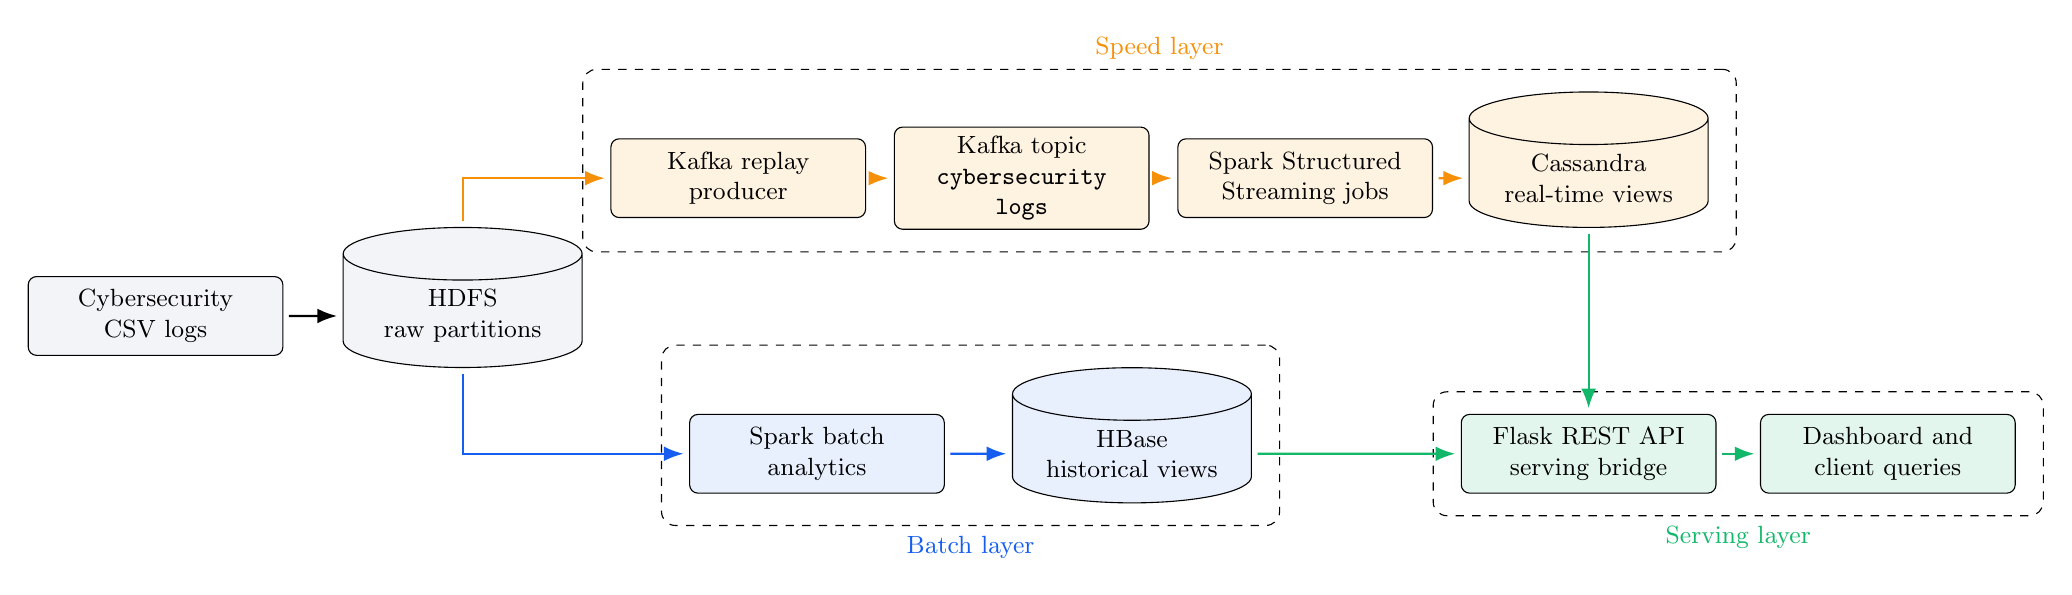
\begin{tikzpicture}[
    font=\small,
    box/.style={draw, rounded corners=3pt, align=center, minimum height=1.0cm, text width=3.0cm, fill=white},
    store/.style={draw, cylinder, shape border rotate=90, aspect=0.22, align=center, minimum height=1.15cm, text width=2.8cm, fill=white},
    layer/.style={draw, rounded corners=5pt, dashed, inner xsep=0.35cm, inner ysep=0.28cm},
    arrow/.style={-{Latex[length=2.5mm]}, thick, shorten >=2pt, shorten <=2pt},
    streamline/.style={arrow, rapidOrange},
    batchline/.style={arrow, rapidBlue},
    serveline/.style={arrow, rapidGreen}
]

\node[box, fill=rapidLight] (dataset) at (0,0) {Cybersecurity\\CSV logs};
\node[store, fill=rapidLight] (hdfs) at (3.9,0) {HDFS\\raw partitions};

\node[box, fill=rapidOrange!12] (producer) at (7.4,1.75) {Kafka replay\\producer};
\node[box, fill=rapidOrange!12] (kafka) at (11.0,1.75) {Kafka topic\\\texttt{cybersecurity}\\\texttt{logs}};
\node[box, fill=rapidOrange!12] (streamjob) at (14.6,1.75) {Spark Structured\\Streaming jobs};
\node[store, fill=rapidOrange!12] (cassandra) at (18.2,1.75) {Cassandra\\real-time views};

\node[box, fill=rapidBlue!10] (batchspark) at (8.4,-1.75) {Spark batch\\analytics};
\node[store, fill=rapidBlue!10] (hbase) at (12.4,-1.75) {HBase\\historical views};

\node[box, fill=rapidGreen!12] (api) at (18.2,-1.75) {Flask REST API\\serving bridge};
\node[box, fill=rapidGreen!12] (dashboard) at (22.0,-1.75) {Dashboard and\\client queries};

\draw[arrow] (dataset) -- (hdfs);
\draw[streamline] (hdfs.north) |- (producer.west);
\draw[streamline] (producer) -- (kafka);
\draw[streamline] (kafka) -- (streamjob);
\draw[streamline] (streamjob) -- (cassandra);

\draw[batchline] (hdfs.south) |- (batchspark.west);
\draw[batchline] (batchspark) -- (hbase);

\draw[serveline] (cassandra.south) -- (api.north);
\draw[serveline] (hbase) -- (api);
\draw[serveline] (api) -- (dashboard);

\begin{scope}[on background layer]
    \node[layer, fit=(producer)(kafka)(streamjob)(cassandra), label={[rapidOrange]above:Speed layer}] {};
    \node[layer, fit=(batchspark)(hbase), label={[rapidBlue]below:Batch layer}] {};
    \node[layer, fit=(api)(dashboard), label={[rapidGreen]below:Serving layer}] {};
\end{scope}

\end{tikzpicture}
}
    \caption{RAPID Lambda Architecture: HDFS keeps replayable raw logs, Kafka carries the live stream, Spark computes batch and speed views, and the Flask API unifies Cassandra and HBase outputs.}
    \label{fig:lambda-architecture}
\end{figure}

\section{Infrastructure Motivation}

The infrastructure design was not chosen only for demonstration. A complete RAPID stack contains Kafka, Zookeeper, HDFS, Spark, Cassandra, HBase, Flask, and the dashboard. Running all of these services on one machine creates resource contention in four places: CPU scheduling, memory pressure, disk input/output, and network ports. This is especially visible in a big-data project because Spark can consume large memory while Cassandra and HBase also need stable heap space, and Kafka/HDFS need reliable disk and network throughput. A single laptop can start the stack in a simplified demo, but it cannot represent the behavior of a real analytical platform under sustained ingestion and processing load.

The project therefore uses a distributed deployment where each machine owns a clear role. This makes the system more realistic: ingestion, compute, serving storage, and API access are separated into different nodes, just as a production data platform separates brokers, compute workers, databases, and application gateways. Figure~\ref{fig:single-host-vs-distributed} summarizes the architectural decision.

\begin{figure}[H]
    \centering
    \resizebox{\textwidth}{!}{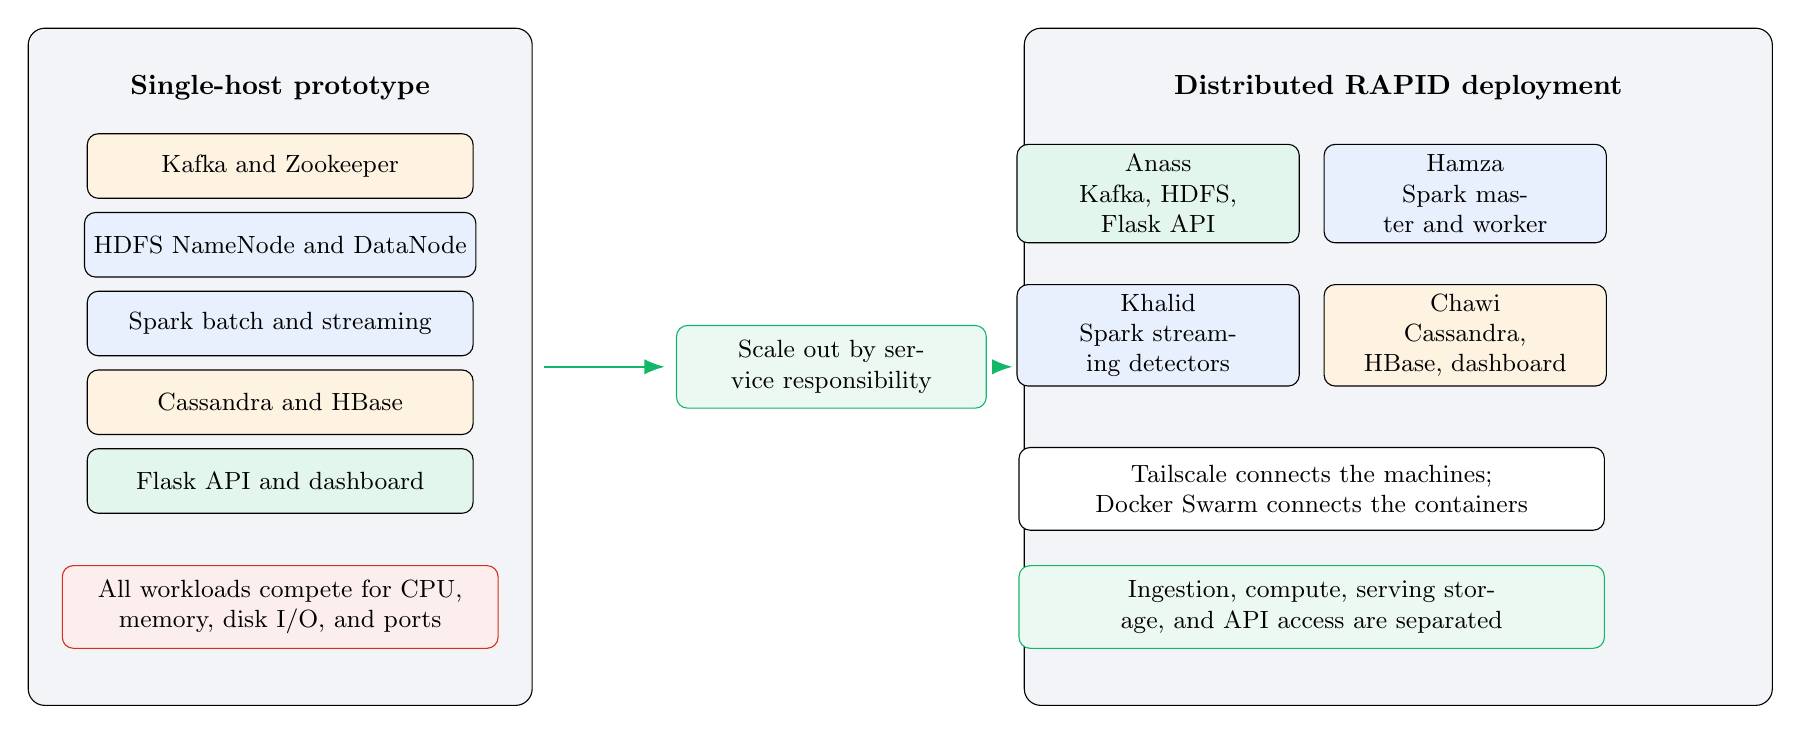
\begin{tikzpicture}[
    font=\small,
    panel/.style={draw, rounded corners=6pt, fill=rapidLight, minimum width=6.4cm, minimum height=8.6cm},
    title/.style={font=\bfseries, align=center},
    service/.style={draw, rounded corners=4pt, align=center, minimum width=4.9cm, minimum height=0.82cm, fill=white},
    host/.style={draw, rounded corners=4pt, align=center, text width=3.35cm, minimum height=1.25cm, fill=white},
    note/.style={draw, rounded corners=4pt, align=center, text width=5.3cm, minimum height=1.05cm, fill=white},
    arrow/.style={-{Latex[length=2.6mm]}, thick, rapidGreen, shorten >=4pt, shorten <=4pt}
]

\node[panel] (singlePanel) at (0,0) {};
\node[title] at (0,3.55) {Single-host prototype};

\node[service, fill=rapidOrange!12] at (0,2.55) {Kafka and Zookeeper};
\node[service, fill=rapidBlue!10] at (0,1.55) {HDFS NameNode and DataNode};
\node[service, fill=rapidBlue!10] at (0,0.55) {Spark batch and streaming};
\node[service, fill=rapidOrange!12] at (0,-0.45) {Cassandra and HBase};
\node[service, fill=rapidGreen!12] at (0,-1.45) {Flask API and dashboard};
\node[note, draw=rapidRed, fill=rapidRed!8] at (0,-3.05) {All workloads compete for CPU, memory, disk I/O, and ports};

\node[note, draw=rapidGreen, fill=rapidGreen!8, text width=3.7cm] (decision) at (7.0,0) {Scale out by service responsibility};

\node[panel, minimum width=9.5cm] (distPanel) at (14.2,0) {};
\node[title] at (14.2,3.55) {Distributed RAPID deployment};

\node[host, fill=rapidGreen!12] at (11.15,2.20) {Anass\\Kafka, HDFS, Flask API};
\node[host, fill=rapidBlue!10] at (15.05,2.20) {Hamza\\Spark master and worker};
\node[host, fill=rapidBlue!10] at (11.15,0.40) {Khalid\\Spark streaming detectors};
\node[host, fill=rapidOrange!12] at (15.05,0.40) {Chawi\\Cassandra, HBase, dashboard};

\node[note, fill=white, text width=7.2cm] at (13.10,-1.55) {Tailscale connects the machines; Docker Swarm connects the containers};
\node[note, draw=rapidGreen, fill=rapidGreen!8, text width=7.2cm] at (13.10,-3.05) {Ingestion, compute, serving storage, and API access are separated};

\draw[arrow] (singlePanel.east) -- (decision.west);
\draw[arrow] (decision.east) -- (distPanel.west);

\end{tikzpicture}
}
    \caption{From a single overloaded host to a distributed deployment where each machine carries a specialized part of the big-data workload.}
    \label{fig:single-host-vs-distributed}
\end{figure}

\section{Scrum Planning and Sprint Backlog}

The implementation was managed through a Scrum-style GitHub project board. The backlog was organized around the same technical layers used by the architecture: batch processing, speed processing, serving integration, visualization, documentation, and infrastructure. This helped the team avoid treating the system as one large undifferentiated task. Each card had an owner, a sprint, and a concrete deliverable, which made the distributed deployment easier to coordinate.


\begin{table}[H]
    \centering
    \caption{Scrum backlog summary extracted from the project planning board.}
    \label{tab:scrum-backlog-summary}
    \begin{tabularx}{\textwidth}{>{\bfseries}l l X}
        \toprule
        Sprint & Main theme & Representative deliverables \\
        \midrule
        Sprint 1 & Batch layer and base infrastructure & Docker environment, partitioned HDFS layout, dataset loading, Spark batch analytics, Cassandra schema, HBase tables, and initial test scripts \\
        Sprint 2 & Speed layer & Kafka topic validation, cross-node Cassandra access, CSV-to-Kafka replay producer, Spark Structured Streaming writers, brute-force detection, signature detection, abnormal-volume detection, and real-time threat scoring \\
        Sprint 3 & Integration and delivery & Flask API endpoints, adaptive scoring, top-10 and timeline views, dashboard pages, end-to-end demonstration script, and technical report material \\
        Sprint 4 & Bonus improvements & MLlib classification, model evaluation, multi-step attack correlation, GeoIP enrichment, and dashboard map visualization \\
        \bottomrule
    \end{tabularx}
\end{table}

Figure~\ref{fig:scrum-board-sprint1} shows the first project-board view. Sprint 1 focused on making the base data platform work: setting up the Docker environment, loading and partitioning the dataset, creating HDFS and HBase structures, and implementing early Spark batch analytics. This sprint reduced the main technical risk because all later work depended on having a stable dataset and reproducible base services.

\begin{figure}[H]
    \centering
    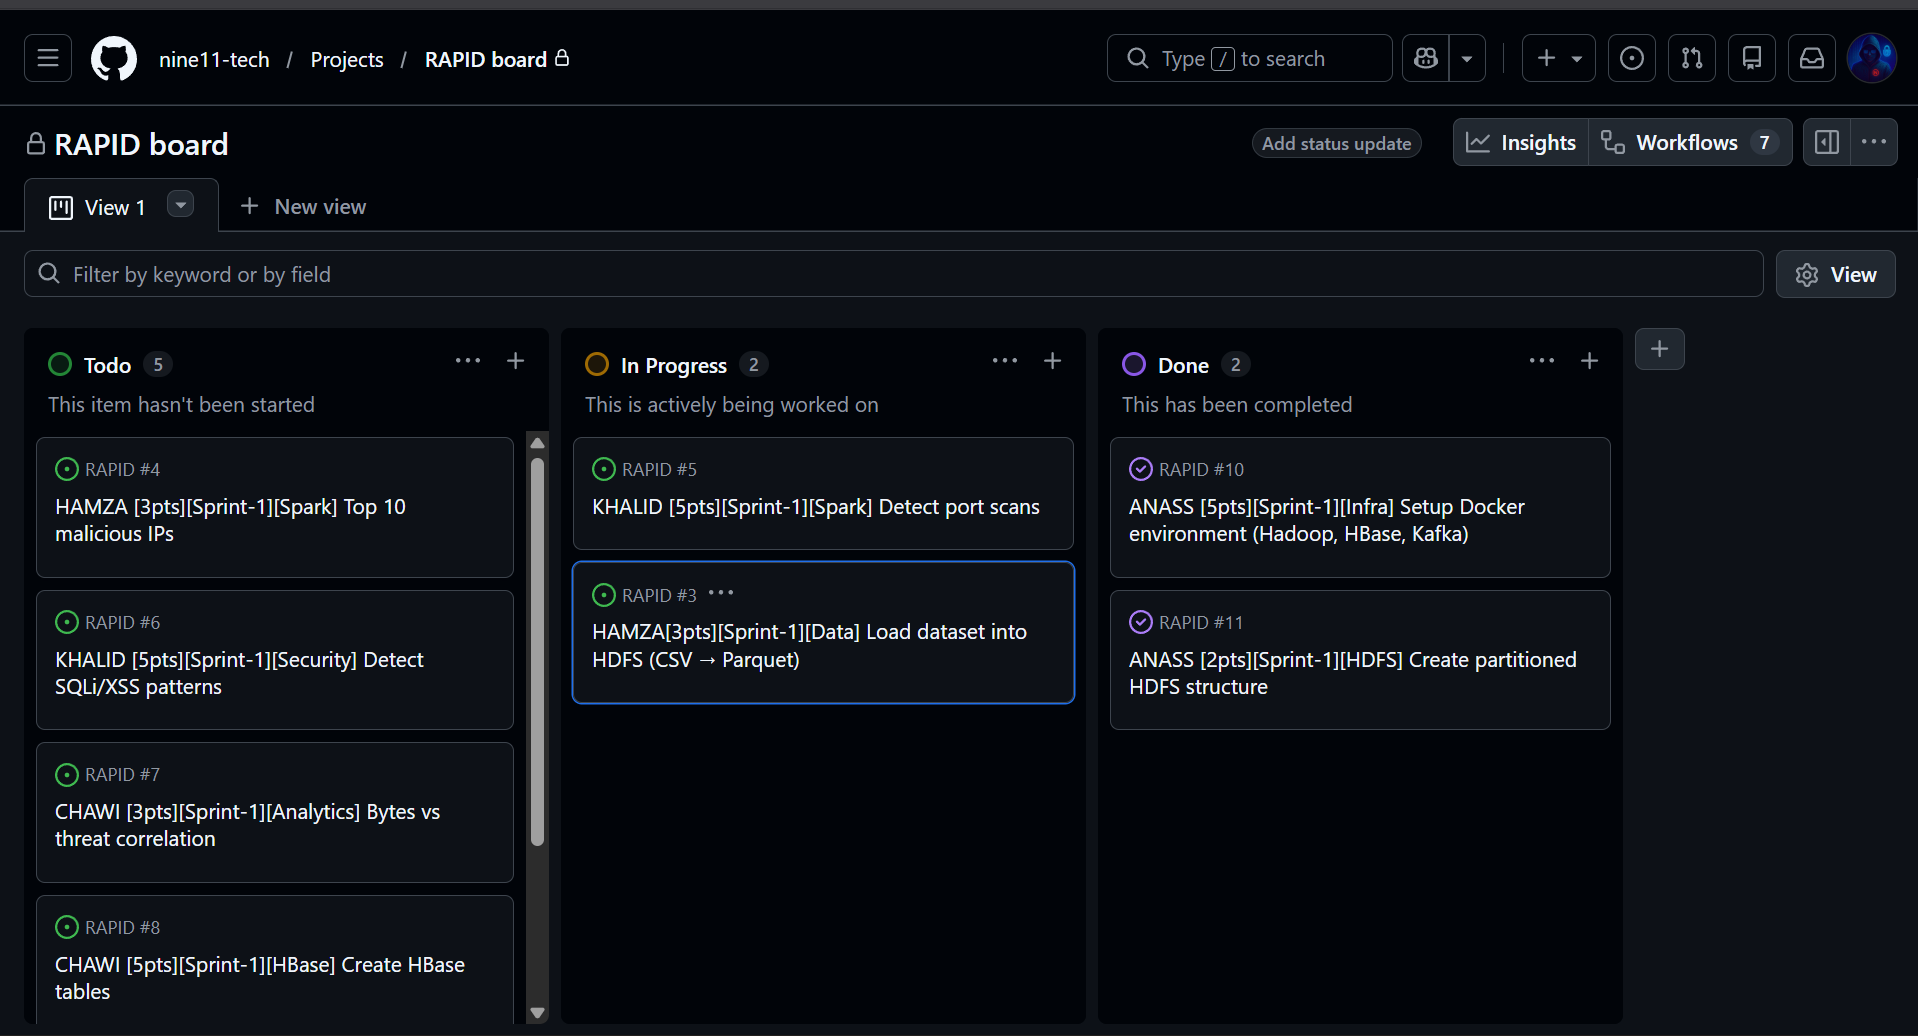
\includegraphics[width=\textwidth]{figures/board1.png}
    \caption{GitHub project board for Sprint 1, focused on the batch layer and base infrastructure.}
    \label{fig:scrum-board-sprint1}
\end{figure}

Figure~\ref{fig:scrum-board-sprint2} shows the second sprint. The board moves the work from offline computation to streaming: Kafka validation, real-time replay from CSV, Spark streaming jobs, Cassandra writes, and detectors for brute-force, signature, and volume-based threats. This sprint is also where cross-machine communication became essential because the streaming container, Kafka broker, and Cassandra service were not all on the same host.

\begin{figure}[H]
    \centering
    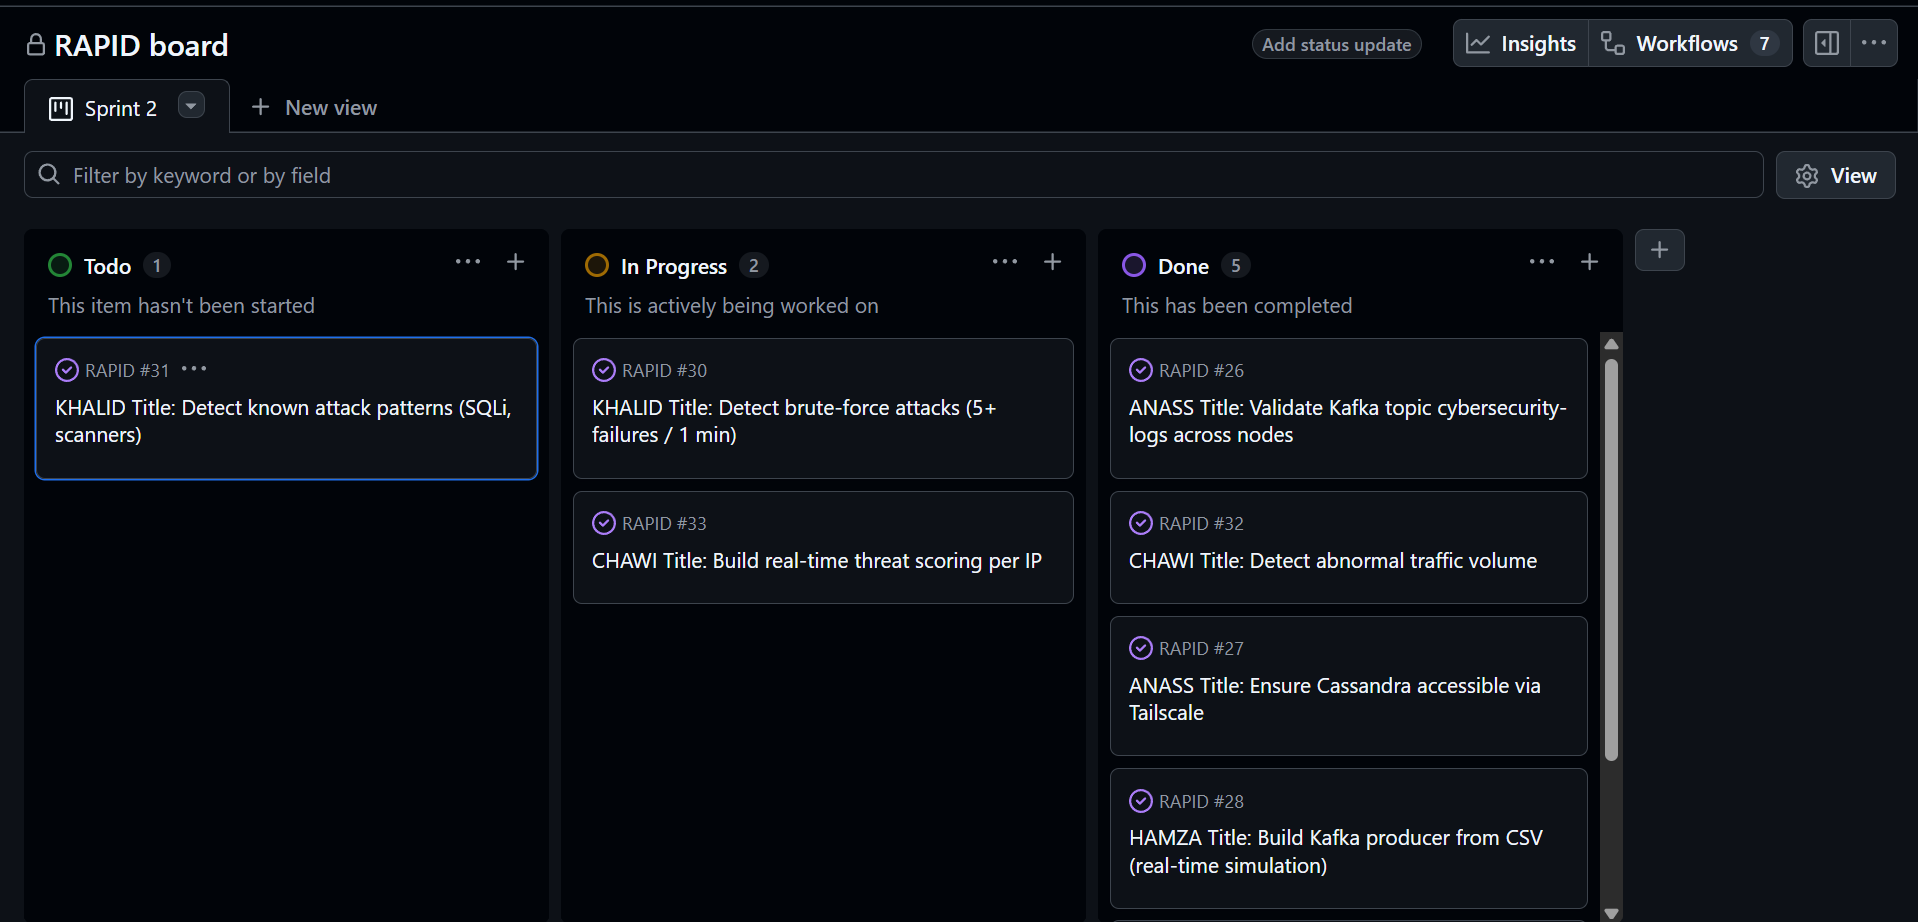
\includegraphics[width=\textwidth]{figures/board2.png}
    \caption{GitHub project board for Sprint 2, focused on Kafka, Spark Streaming, Cassandra writes, and real-time detectors.}
    \label{fig:scrum-board-sprint2}
\end{figure}

Figure~\ref{fig:scrum-board-sprint3} shows the third sprint. The tasks shifted toward integration: API endpoints, adaptive scoring, dashboard pages, an end-to-end demo, and the written technical report. This sprint connected the individual layer outputs into a user-facing security monitoring workflow.

\begin{figure}[H]
    \centering
    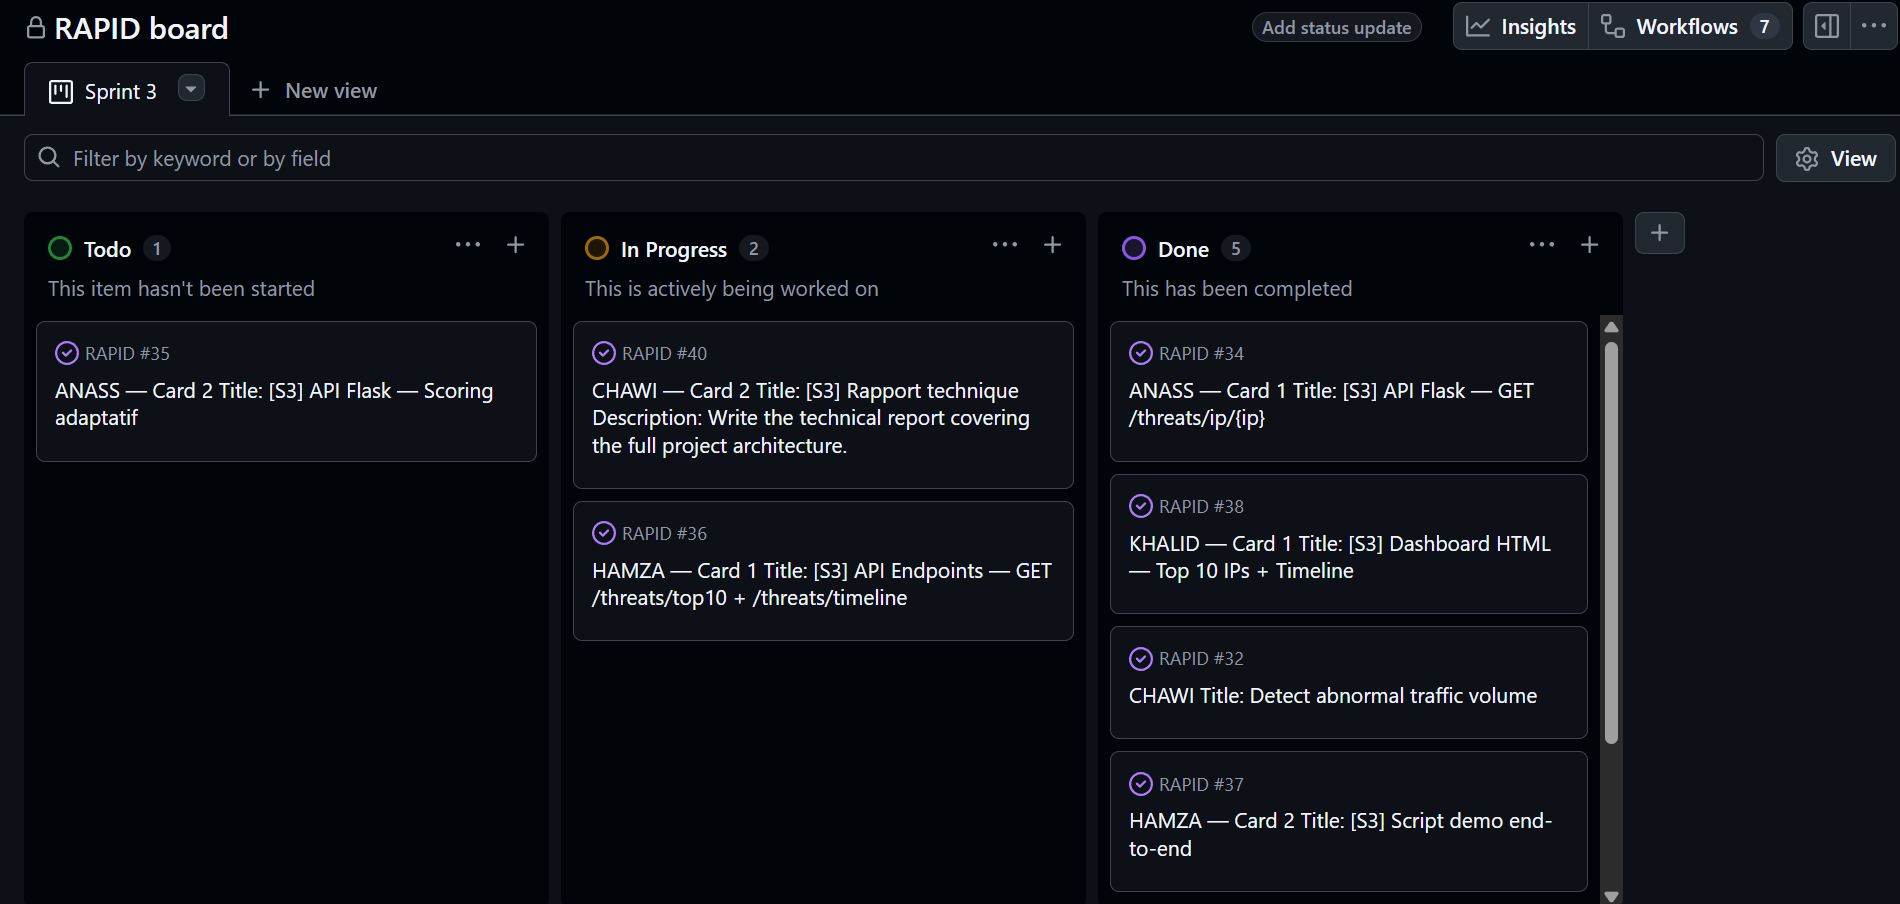
\includegraphics[width=\textwidth]{figures/board3.png}
    \caption{GitHub project board for Sprint 3, focused on API integration, dashboard delivery, demonstration, and reporting.}
    \label{fig:scrum-board-sprint3}
\end{figure}

\section{Tailscale and Docker Swarm Infrastructure}

The deployment uses two complementary networking mechanisms. Tailscale provides the private network between physical machines. Docker Swarm provides the container-level overlay network. These two layers solve different problems and are both necessary.

\subsection{Why Tailscale Is Used}

Tailscale gives each team machine a stable private address in the \texttt{100.x.x.x} range. This is important because the team is not working inside a single university data center with fixed servers. The machines may be on different local networks, behind NAT, or connected from different places. Without Tailscale, the team would have to expose ports publicly, configure router forwarding, or constantly change IP addresses in scripts and containers. That would make the deployment fragile and less secure.

With Tailscale, Kafka can be advertised as \texttt{100.73.216.115:9092}, Cassandra can be reached at \texttt{100.97.208.110:9042}, HBase Thrift can be reached at \texttt{100.97.208.110:9090}, and the Flask API can expose \texttt{100.73.216.115:5000}. This makes the distributed infrastructure predictable. It also keeps communication private because the services are intended to be accessed through the Tailscale mesh rather than through public Internet addresses \cite{tailscale_docs}.

\subsection{Why Docker Swarm Is Used}

Docker Compose alone is comfortable for a single host, but RAPID is intentionally multi-host. Docker Swarm adds the cluster concept needed to connect containers across machines \cite{docker_swarm_docs}. The external attachable network \texttt{rapid-overlay} allows containers started by different Compose profiles to communicate through one logical overlay. This means that a Spark container on one machine can reach Kafka on Anass' node and Cassandra on Chawi's node without pretending that all services are local.

The Compose profiles also enforce ownership. Anass starts only the \texttt{anass} profile, Hamza starts \texttt{hamza}, Khalid starts \texttt{khalid}, and Chawi starts \texttt{chawi}. This is cleaner than asking every team member to run the full infrastructure. It also mirrors real deployments where different teams or nodes own different services.

\begin{figure}[H]
    \centering
    \resizebox{\textwidth}{!}{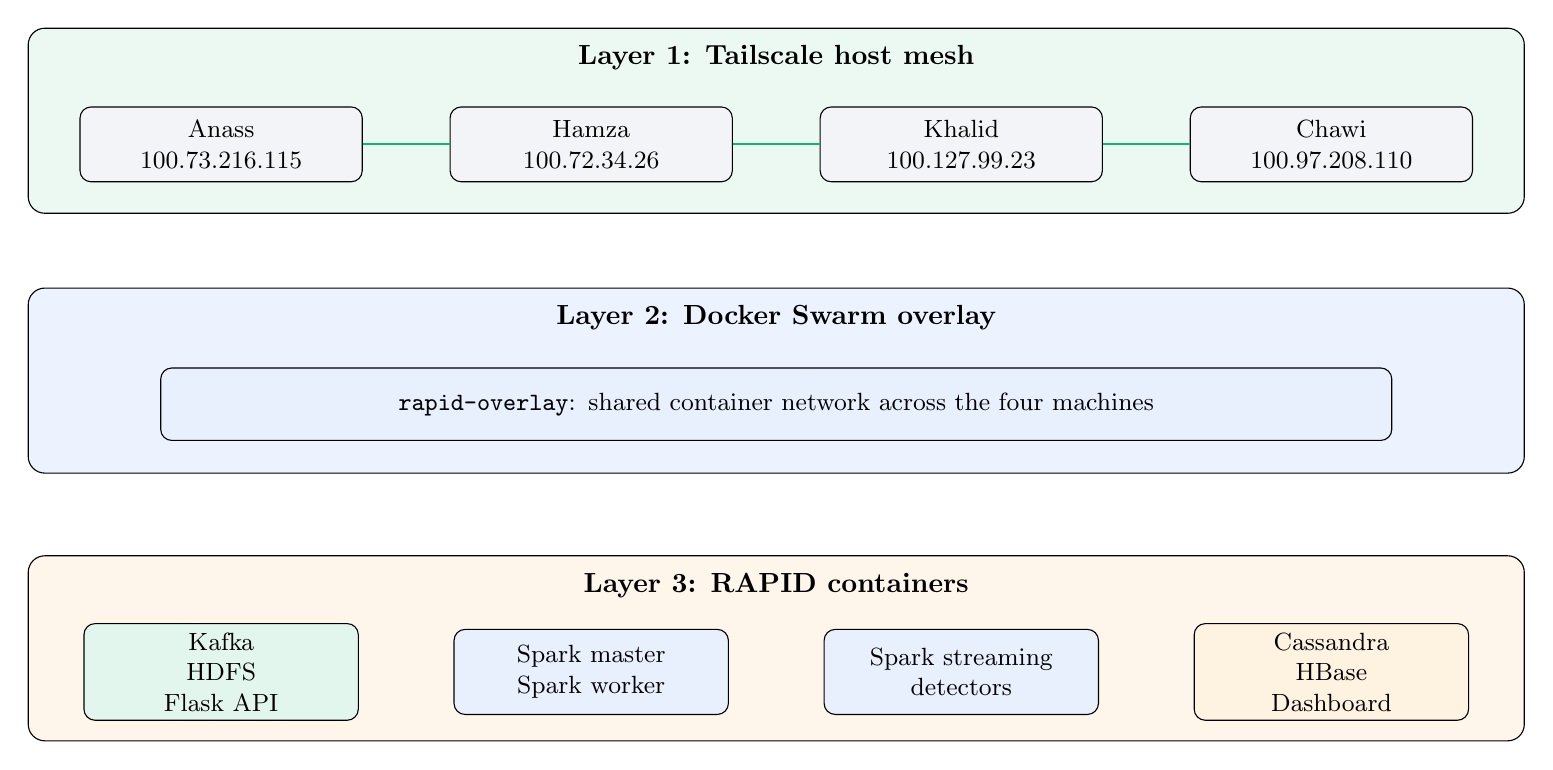
\begin{tikzpicture}[
    font=\small,
    layer/.style={draw, rounded corners=6pt, minimum width=19.0cm, minimum height=2.35cm, fill=white},
    layername/.style={font=\bfseries, align=center},
    host/.style={draw, rounded corners=4pt, align=center, text width=3.35cm, minimum height=0.95cm, fill=white},
    service/.style={draw, rounded corners=4pt, align=center, text width=3.25cm, minimum height=1.08cm, fill=white},
    overlay/.style={draw, rounded corners=4pt, align=center, text width=15.4cm, minimum height=0.92cm, fill=rapidBlue!10},
    mesh/.style={thick, rapidGreen}
]

\node[layer, fill=rapidGreen!8] at (0,3.85) {};
\node[layername] at (0,4.65) {Layer 1: Tailscale host mesh};
\node[host, fill=rapidLight] (anassIp) at (-7.05,3.55) {Anass\\100.73.216.115};
\node[host, fill=rapidLight] (hamzaIp) at (-2.35,3.55) {Hamza\\100.72.34.26};
\node[host, fill=rapidLight] (khalidIp) at (2.35,3.55) {Khalid\\100.127.99.23};
\node[host, fill=rapidLight] (chawiIp) at (7.05,3.55) {Chawi\\100.97.208.110};

\draw[mesh] (anassIp.east) -- (hamzaIp.west);
\draw[mesh] (hamzaIp.east) -- (khalidIp.west);
\draw[mesh] (khalidIp.east) -- (chawiIp.west);

\node[layer, fill=rapidBlue!8] at (0,0.55) {};
\node[layername] at (0,1.35) {Layer 2: Docker Swarm overlay};
\node[overlay] (rapidOverlay) at (0,0.25) {\texttt{rapid-overlay}: shared container network across the four machines};

\node[layer, fill=rapidOrange!8] at (0,-2.85) {};
\node[layername] at (0,-2.05) {Layer 3: RAPID containers};
\node[service, fill=rapidGreen!12] (anassSvc) at (-7.05,-3.15) {Kafka\\HDFS\\Flask API};
\node[service, fill=rapidBlue!10] (hamzaSvc) at (-2.35,-3.15) {Spark master\\Spark worker};
\node[service, fill=rapidBlue!10] (khalidSvc) at (2.35,-3.15) {Spark streaming\\detectors};
\node[service, fill=rapidOrange!12] (chawiSvc) at (7.05,-3.15) {Cassandra\\HBase\\Dashboard};

\end{tikzpicture}
}
    \caption{Infrastructure layers: Tailscale connects the physical machines, while Docker Swarm provides the shared container overlay network.}
    \label{fig:tailscale-swarm-layers}
\end{figure}

\subsection{Operational Verification from Docker Screenshots}

The Docker Swarm deployment was verified from the command line by checking both node membership and running containers. Figure~\ref{fig:docker-node-status} shows that the machines were registered in the Swarm membership list. In that capture, some worker nodes appear as \texttt{Down}; this does not invalidate the deployment model, because student laptops can be temporarily offline, suspended, or disconnected from Tailscale when the manager runs \texttt{docker node ls}. For that reason, the stronger operational evidence is the per-machine \texttt{docker ps} output in Figures~\ref{fig:docker-ps-anass}--\ref{fig:docker-ps-chawi}, which shows the actual containers running on each owner machine.

\begin{figure}[H]
    \centering
    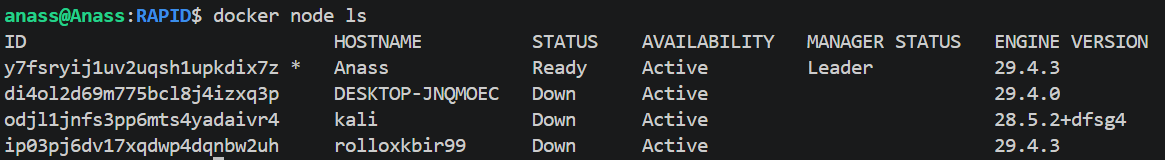
\includegraphics[width=\textwidth]{figures/dockernode.png}
    \caption{Docker Swarm node list on the manager machine. The list verifies node registration; temporary \texttt{Down} states reflect machine availability at screenshot time.}
    \label{fig:docker-node-status}
\end{figure}

\begin{figure}[H]
    \centering
    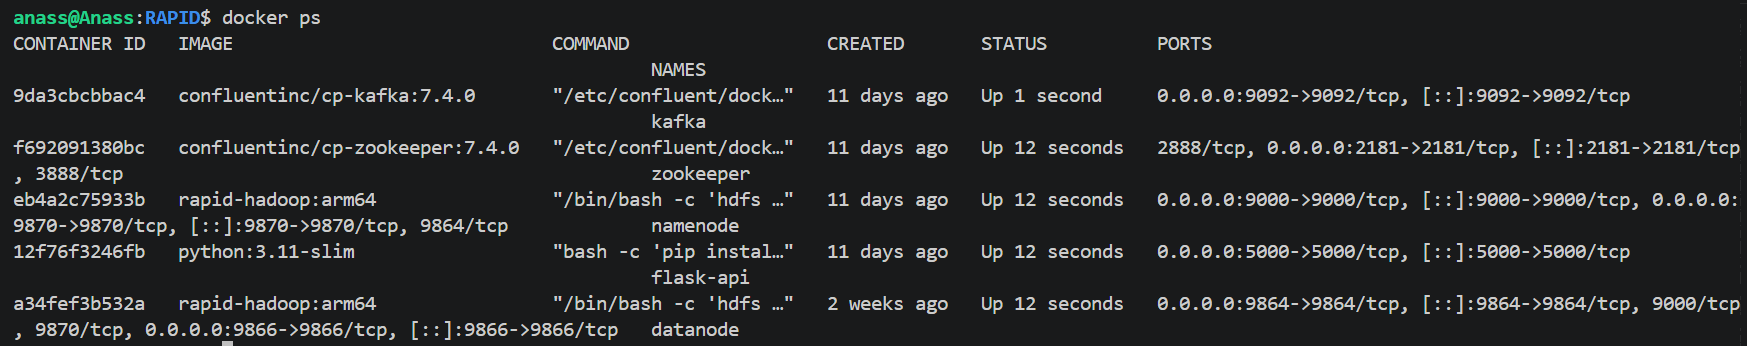
\includegraphics[width=\textwidth]{figures/dockerps1.png}
    \caption{Docker container status on Anass' machine, showing Kafka, Zookeeper, HDFS NameNode/DataNode, and the Flask API profile.}
    \label{fig:docker-ps-anass}
\end{figure}

\begin{figure}[H]
    \centering
    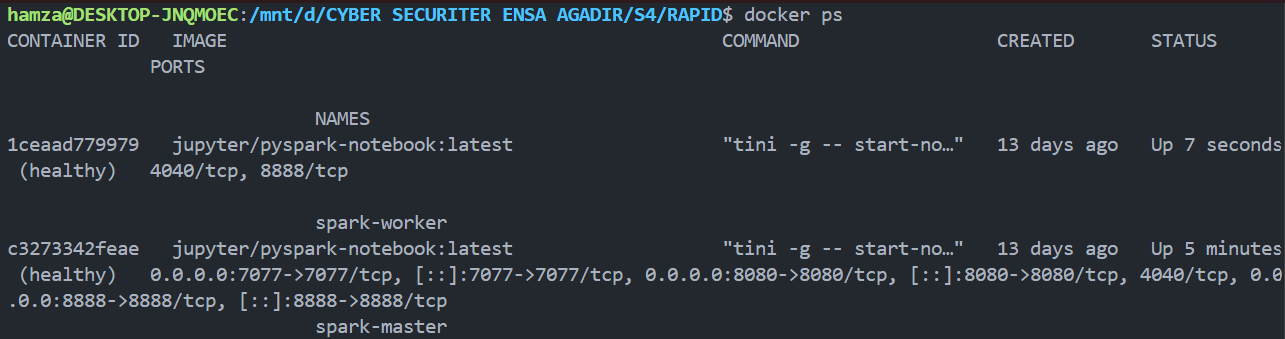
\includegraphics[width=\textwidth]{figures/docker_ps_hamza.png}
    \caption{Docker container status on Hamza's machine, showing the Spark master and Spark worker used for batch processing and Kafka replay work.}
    \label{fig:docker-ps-hamza}
\end{figure}

\begin{figure}[H]
    \centering
    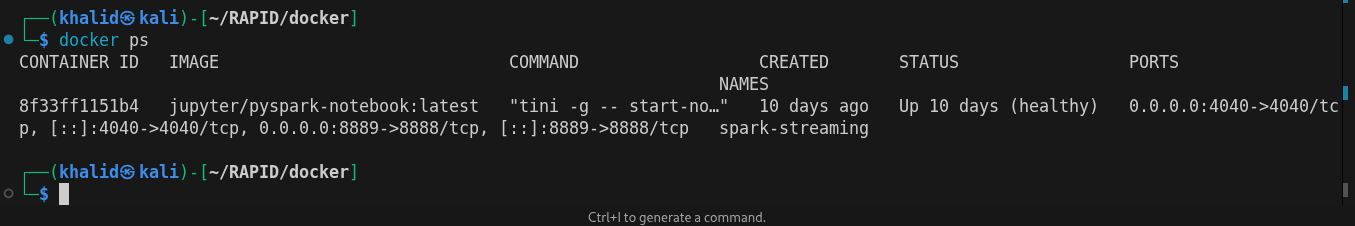
\includegraphics[width=\textwidth]{figures/docker_ps.png}
    \caption{Docker container status on Khalid's machine, showing the single Spark streaming container used for real-time detection jobs.}
    \label{fig:docker-ps-khalid}
\end{figure}

\begin{figure}[H]
    \centering
    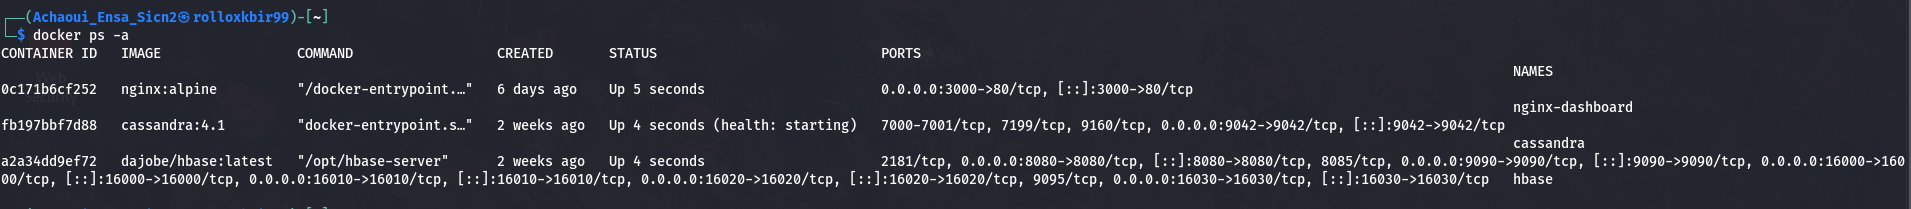
\includegraphics[width=\textwidth]{figures/docker_ps_chawi.png}
    \caption{Docker container status on Chawi's machine, showing Cassandra, HBase, and the Nginx dashboard container for the serving and visualization layer.}
    \label{fig:docker-ps-chawi}
\end{figure}

Together, these screenshots support the architectural claim made in the backlog: every member does not need to run the full stack. Anass carries the infrastructure gateway services, Hamza carries Spark batch execution, Khalid carries the lightweight streaming runtime, and Chawi carries the serving databases and dashboard host. The distribution is especially important for machines with lower memory capacity, because Cassandra, HBase, and Spark should not all be forced onto the same laptop during the demonstration.

\subsection{Runtime Communication}

Figure~\ref{fig:runtime-communication} shows how the services communicate during execution. The important point is that no component is isolated: Spark batch jobs read from HDFS and write HBase views, streaming jobs consume Kafka and write Cassandra views, and the Flask API reads both databases to serve the dashboard. The architecture therefore behaves like a small production cluster rather than a monolithic local script.

\begin{figure}[H]
    \centering
    \resizebox{\textwidth}{!}{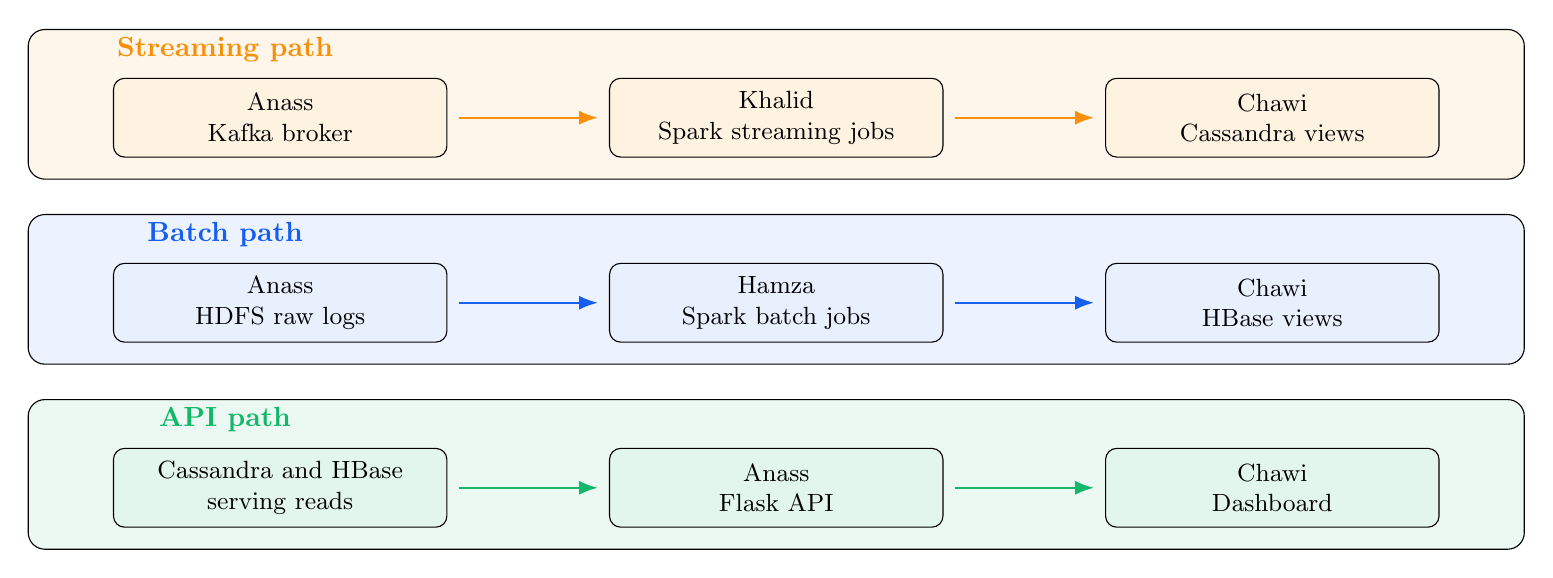
\begin{tikzpicture}[
    font=\small,
    lane/.style={draw, rounded corners=6pt, minimum width=19.0cm, minimum height=1.9cm, fill=white},
    lanetitle/.style={font=\bfseries, align=left},
    svc/.style={draw, rounded corners=4pt, align=center, text width=4.0cm, minimum height=1.0cm, fill=white},
    arrow/.style={-{Latex[length=2.4mm]}, thick, shorten >=4pt, shorten <=4pt},
    stream/.style={arrow, rapidOrange},
    batch/.style={arrow, rapidBlue},
    query/.style={arrow, rapidGreen}
]

% Streaming lane.
\node[lane, fill=rapidOrange!8] at (0,2.35) {};
\node[lanetitle, text=rapidOrange] at (-7.0,3.05) {Streaming path};
\node[svc, fill=rapidOrange!12] (kafka) at (-6.3,2.18) {Anass\\Kafka broker};
\node[svc, fill=rapidOrange!12] (streaming) at (0,2.18) {Khalid\\Spark streaming jobs};
\node[svc, fill=rapidOrange!12] (cassWrite) at (6.3,2.18) {Chawi\\Cassandra views};
\draw[stream] (kafka.east) -- (streaming.west);
\draw[stream] (streaming.east) -- (cassWrite.west);

% Batch lane.
\node[lane, fill=rapidBlue!8] at (0,0) {};
\node[lanetitle, text=rapidBlue] at (-7.0,0.70) {Batch path};
\node[svc, fill=rapidBlue!10] (hdfs) at (-6.3,-0.17) {Anass\\HDFS raw logs};
\node[svc, fill=rapidBlue!10] (batchJobs) at (0,-0.17) {Hamza\\Spark batch jobs};
\node[svc, fill=rapidBlue!10] (hbase) at (6.3,-0.17) {Chawi\\HBase views};
\draw[batch] (hdfs.east) -- (batchJobs.west);
\draw[batch] (batchJobs.east) -- (hbase.west);

% Query lane.
\node[lane, fill=rapidGreen!8] at (0,-2.35) {};
\node[lanetitle, text=rapidGreen] at (-7.0,-1.65) {API path};
\node[svc, fill=rapidGreen!12] (stores) at (-6.3,-2.52) {Cassandra and HBase\\serving reads};
\node[svc, fill=rapidGreen!12] (api) at (0,-2.52) {Anass\\Flask API};
\node[svc, fill=rapidGreen!12] (dashboard) at (6.3,-2.52) {Chawi\\Dashboard};
\draw[query] (stores.east) -- (api.west);
\draw[query] (api.east) -- (dashboard.west);

\end{tikzpicture}
}
    \caption{Runtime communication between owner nodes. The arrows represent the main data and query paths used by the RAPID pipeline.}
    \label{fig:runtime-communication}
\end{figure}

\subsection{Physical Deployment}

The physical deployment uses stable private IP addresses instead of assuming that all services run on the same host. Table~\ref{tab:deployment-ownership} summarizes the ownership model. The Anass profile is the entry point of the data backbone because Kafka, HDFS, and the API are the services that connect the other layers together.

\begin{table}[H]
    \centering
    \caption{Distributed service ownership in the RAPID deployment.}
    \label{tab:deployment-ownership}
    \begin{tabularx}{\textwidth}{>{\bfseries}l l X}
        \toprule
        Owner & Tailscale address & Main services \\
        \midrule
        Anass & \texttt{100.73.216.115} & Zookeeper, Kafka broker, HDFS NameNode, HDFS DataNode, Flask REST API \\
        Hamza & \texttt{100.72.34.26} & Spark master, Spark worker, Jupyter/Spark development environment \\
        Khalid & \texttt{100.127.99.23} & Spark streaming container and real-time detection jobs \\
        Chawi & \texttt{100.97.208.110} & Cassandra, HBase Thrift service, HBase UI, dashboard hosting \\
        \bottomrule
    \end{tabularx}
\end{table}

This deployment model provides a practical simulation of real-life big-data infrastructure. A production platform normally does not place brokers, distributed storage, compute engines, serving databases, and APIs on one machine. RAPID follows the same principle at project scale. The platform separates concerns, keeps the raw data and derived views rebuildable, and gives every service a clear network endpoint.

\section{Rationale for a Lambda Architecture}

A cybersecurity monitoring system must answer two different classes of questions. Some questions are historical: which IP addresses were repeatedly malicious during the month, which protocols were most affected, and which attack patterns were observed across the dataset? Other questions are operational: did a source IP just trigger a brute-force pattern, is the current volume abnormal, and should the dashboard recommend blocking or monitoring an IP? A single processing model is poorly suited to both workloads. Batch processing provides accuracy and completeness, but it is not optimized for immediate alerts. Pure streaming provides freshness, but it is less convenient for recomputing large historical views when logic changes or when late data is found.

The Lambda Architecture separates these concerns into a batch layer, a speed layer, and a serving layer \cite{marz2011lambda,marz2015bigdata}. RAPID applies this idea as follows:

\begin{itemize}
    \item The \textbf{batch layer} reads the complete log corpus from HDFS and computes historical indicators such as IP reputation, attack patterns, threat timelines, port-scan summaries, and volume-by-threat statistics.
    \item The \textbf{speed layer} consumes events from Kafka and updates Cassandra with recent logs, signature alerts, volume alerts, brute-force detections, and threat scores.
    \item The \textbf{serving layer} exposes both views through Flask. The API does not force the client to know whether an answer is historical or real-time; it joins the relevant evidence and returns a decision-ready JSON document.
\end{itemize}

This design also supports replay. Since the producer reads HDFS partitions and publishes events to Kafka, the team can replay the dataset into the speed layer after changing a streaming rule. Reproducibility is essential in an academic project because the same dataset can be used to verify each processing stage under controlled conditions.

\section{Technology Choices}

\subsection{Kafka for Ingestion and Decoupling}

Kafka was selected as the ingestion backbone because it is designed for durable, ordered event streams and for decoupling producers from consumers \cite{kafka_docs}. In RAPID, the topic \texttt{cybersecurity-logs} receives JSON events generated from HDFS monthly partitions. The Kafka producer uses \texttt{source\_ip} as the message key, which keeps related events naturally grouped for downstream processing. The producer also maintains a small state file so that an interrupted replay can resume from the last month and line number instead of restarting the full dataset.

The main architectural benefit of Kafka is that it protects the streaming jobs from direct dependency on HDFS reads. Spark streaming jobs consume from Kafka at their own pace, and additional detection jobs can be attached to the same topic without changing the producer. For security analytics, this matters because new detectors are often added iteratively: a brute-force detector, a signature detector, a volume detector, and a score aggregator can all observe the same event stream while writing separate serving tables.

\subsection{HDFS for the Raw, Replayable Dataset}

HDFS is used as the durable storage layer for the raw cybersecurity logs. The current convention stores monthly partitions under paths such as \texttt{/logs/year=2024/month=01/data.csv}. HDFS is appropriate here because it is built for large files, sequential reads, and distributed storage \cite{hdfs_docs}. The partition layout makes it possible to process the complete dataset for batch analytics and to replay selected months through Kafka when validating the speed layer.

The role of HDFS is not only storage capacity. It is also the audit base of the architecture. If a derived table in Cassandra or HBase becomes inconsistent, the raw partitioned data remains available for recomputation. This property is a core reason why Lambda Architecture is useful in analytical systems: derived views can be rebuilt from immutable input data when algorithms evolve.

\subsection{Spark for Unified Batch and Streaming Computation}

Spark was selected because it provides a single programming environment for batch processing and streaming analytics \cite{spark_docs}. The batch jobs in \texttt{spark/batch/} compute historical views such as malicious IP rankings, port scans, attack paths, HBase threat timelines, multi-step attacks, and volume statistics. The streaming jobs in \texttt{spark/streaming/} consume Kafka using Structured Streaming and write results to Cassandra \cite{spark_streaming_docs}.

Using Spark in both layers reduces conceptual fragmentation. The same schema fields, such as \texttt{timestamp}, \texttt{source\_ip}, \texttt{dest\_ip}, \texttt{protocol}, \texttt{action}, \texttt{threat\_label}, \texttt{bytes\_transferred}, \texttt{user\_agent}, and \texttt{request\_path}, are transformed across the batch and speed jobs. This makes the results easier to compare and makes future maintenance simpler.

\subsection{Cassandra for Real-Time Serving Views}

Cassandra was selected for the speed layer serving store because it is a distributed wide-column database optimized for high-write workloads and predictable key-based reads \cite{cassandra_docs}. RAPID's streaming jobs write frequently updated operational views into the \texttt{cybersecurity} keyspace. The Flask API reads from tables such as \texttt{logs}, \texttt{realtime\_threats}, \texttt{signature\_alerts}, \texttt{volume\_alerts}, and \texttt{threat\_scores}.

The data model follows the access patterns of the API. For example, \texttt{/threats/ip/<ip>} reads the latest real-time threat state, score, signature alerts, and volume alerts for a source IP. \texttt{/threats/top10} scans the scoring table and sorts the highest-risk sources for dashboard presentation. The design favors fast operational lookup over ad-hoc relational joins, which is consistent with Cassandra's strengths.

\subsection{HBase for Historical Reputation and Time-Series Views}

HBase was selected for historical and batch-generated views because it provides sparse, versioned, column-family-oriented storage on top of the Hadoop ecosystem \cite{hbase_docs}. In RAPID, HBase stores tables such as \texttt{ip\_reputation}, \texttt{attack\_patterns}, and \texttt{threat\_timeline}. These tables are produced by batch jobs and accessed through the HBase Thrift service from the Flask API.

HBase complements Cassandra rather than replacing it. Cassandra serves recent state generated by the streaming layer, while HBase stores historical evidence computed from the complete dataset. For instance, the API uses HBase \texttt{ip\_reputation} values such as threat counts, SQL injection hits, tool hits, traversal hits, cross-site scripting hits, and average transferred bytes to calculate a normalized historical score. This historical score is then compared with current Cassandra scores to produce a final decision.

\section{Data Flow and Processing Contracts}

The architecture relies on explicit contracts between stages. The ingestion schema contains the timestamp, source and destination IP addresses, protocol, action, threat label, log type, transferred bytes, user agent, and request path. These fields are carried as JSON through Kafka and converted by Spark into typed columns. The base streaming writer persists the raw stream into Cassandra \texttt{logs}; specialized jobs then derive detector-specific tables.

\begin{longtable}{
    >{\raggedright\arraybackslash\bfseries}p{0.23\textwidth}
    >{\raggedright\arraybackslash}p{0.29\textwidth}
    >{\raggedright\arraybackslash}p{0.36\textwidth}
}
    \caption{Main data contracts between RAPID components.}
    \label{tab:data-contracts}\\
    \toprule
    Contract & Producer & Consumer or destination \\
    \midrule
    \endfirsthead
    \toprule
    Contract & Producer & Consumer or destination \\
    \midrule
    \endhead
    HDFS raw partitions & Dataset loader and storage preparation scripts & Kafka replay producer and Spark batch jobs \\
    Kafka JSON events & \texttt{spark/speed\_layer/}\newline\texttt{kafka\_producer.py} & Spark streaming writer and detection jobs \\
    Cassandra raw logs & Base streaming writer & API timeline, protocol aggregation, adaptive threshold, geo endpoint \\
    Cassandra alert views & Signature, brute-force, volume, and score streaming jobs & API threat lookup, recent alerts, top 10, volume endpoint \\
    HBase historical views & Spark batch jobs & API historical reputation and long-term trend lookup \\
    REST JSON responses & Flask API & Dashboard, smoke tests, integration tests, and external clients \\
    \bottomrule
\end{longtable}

This contract-based design reduces coupling. For example, a new streaming detector can write a new Cassandra view without changing the raw HDFS layout. Similarly, a batch job can improve the HBase reputation formula while the REST endpoint continues to return the same high-level fields to the dashboard.

\section{Flask API as the Serving Bridge}

The Flask API is the integration point between storage systems and client applications \cite{flask_docs}. It runs on Anass' node and connects to Cassandra and HBase through environment-configured hosts. Its purpose is not merely to expose database rows; it transforms distributed evidence into a security decision. Figure~\ref{fig:api-bridge} shows this bridge.

\begin{figure}[H]
    \centering
    \resizebox{\textwidth}{!}{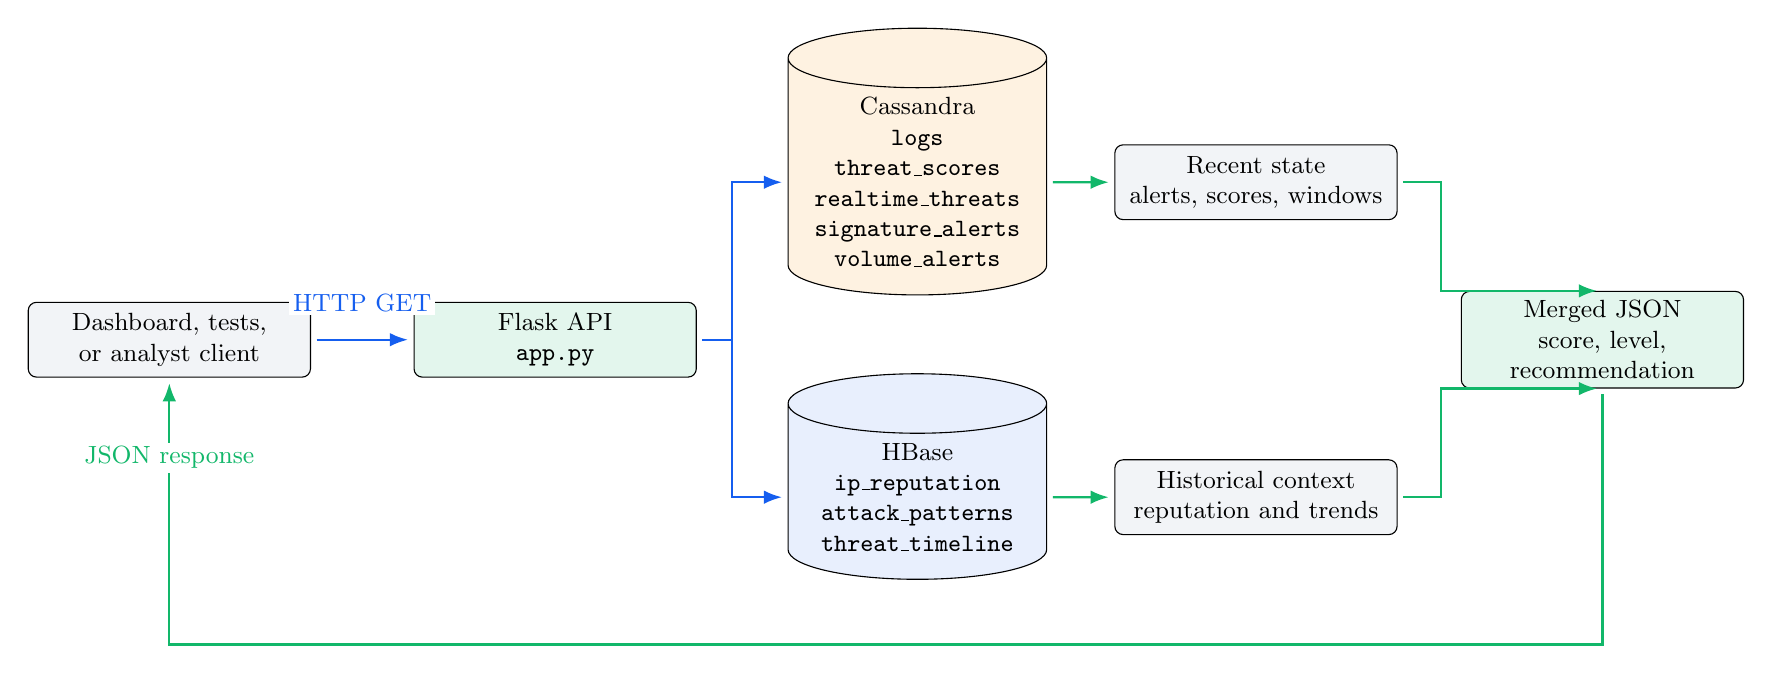
\begin{tikzpicture}[
    font=\small,
    box/.style={draw, rounded corners=3pt, align=center, minimum height=0.95cm, text width=3.35cm, fill=white},
    db/.style={draw, cylinder, shape border rotate=90, aspect=0.23, align=center, minimum height=1.1cm, text width=3.05cm, fill=white},
    arrow/.style={-{Latex[length=2.3mm]}, thick, shorten >=2pt, shorten <=2pt},
    query/.style={arrow, rapidBlue},
    result/.style={arrow, rapidGreen}
]

\node[box, fill=rapidLight] (client) at (0,0) {Dashboard, tests,\\or analyst client};
\node[box, fill=rapidGreen!12] (flask) at (4.9,0) {Flask API\\\texttt{app.py}};

\node[db, fill=rapidOrange!12] (cass) at (9.5,2.0) {Cassandra\\\texttt{logs}\\\texttt{threat\_scores}\\\texttt{realtime\_threats}\\\texttt{signature\_alerts}\\\texttt{volume\_alerts}};
\node[db, fill=rapidBlue!10] (hbase) at (9.5,-2.0) {HBase\\\texttt{ip\_reputation}\\\texttt{attack\_patterns}\\\texttt{threat\_timeline}};

\node[box, fill=rapidLight] (rt) at (13.8,2.0) {Recent state\\alerts, scores, windows};
\node[box, fill=rapidLight] (hist) at (13.8,-2.0) {Historical context\\reputation and trends};
\node[box, fill=rapidGreen!12] (decision) at (18.2,0) {Merged JSON\\score, level,\\recommendation};

\draw[query] (client) -- (flask);
\node[fill=white, inner sep=1.5pt, text=rapidBlue] at (2.45,0.47) {HTTP GET};
\draw[query] (flask.east) -- ++(0.45,0) |- (cass.west);
\draw[query] (flask.east) -- ++(0.45,0) |- (hbase.west);

\draw[result] (cass) -- (rt);
\draw[result] (hbase) -- (hist);
\draw[result] (rt.east) -- ++(0.55,0) |- (decision.north);
\draw[result] (hist.east) -- ++(0.55,0) |- (decision.south);
\draw[result] (decision.south) |- ++(0,-3.25) -| node[pos=0.88, below, fill=white, inner sep=1.5pt]{JSON response} (client.south);

\end{tikzpicture}
}
    \caption{Flask API bridge: operational Cassandra views and historical HBase views are merged into decision-ready JSON responses.}
    \label{fig:api-bridge}
\end{figure}

\subsection{Connection Strategy}

The API keeps a persistent Cassandra session with a lightweight health query before reuse. If the session fails, it shuts down the old cluster handle and reconnects. This is useful in a distributed student deployment where containers may restart independently. HBase access is performed through HappyBase over the Thrift port \texttt{9090}. The environment variables \texttt{CASSANDRA\_HOST}, \texttt{HBASE\_HOST}, and \texttt{HDFS\_HOST} allow the same API code to run even if the physical node addresses change.

\subsection{Endpoint Responsibilities}

Table~\ref{tab:api-endpoints} summarizes the endpoints implemented in \texttt{bigdata-api/app.py}. The most important endpoint is \texttt{/threats/ip/<ip>} because it demonstrates the bridge between databases. It queries Cassandra for real-time state and HBase for historical reputation, computes a final score, compares it with the adaptive threshold, and returns a recommendation.

\begin{longtable}{>{\ttfamily}p{0.29\textwidth} p{0.27\textwidth} p{0.34\textwidth}}
    \caption{Flask API endpoints and their role in the serving layer.}
    \label{tab:api-endpoints}\\
    \toprule
    Endpoint & Main data source & Returned information \\
    \midrule
    \endfirsthead
    \toprule
    Endpoint & Main data source & Returned information \\
    \midrule
    \endhead
    GET /health & Runtime configuration & API status, backend hosts, HBase port, Cassandra keyspace \\
    GET /threats/ip/<ip> & Cassandra and HBase & Real-time threats, threat score, signatures, volume alerts, historical reputation, final score, threat level, recommendation \\
    GET /threats/top10 & Cassandra \texttt{threat\_scores} & Highest scored source IPs with malicious, suspicious, and total event counts \\
    GET /threats/threshold & Cassandra \texttt{logs} & Rolling 24-hour adaptive threshold and calculation metadata \\
    GET /threats/recent & Cassandra \texttt{signature\_alerts} & Most recent signature-based alerts \\
    GET /threats/volume-alerts & Cassandra \texttt{volume\_alerts} & Recent traffic-volume anomalies and detection windows \\
    GET /threats/by-protocol & Cassandra \texttt{logs} & Total, malicious, and suspicious counts grouped by protocol \\
    GET /threats/timeline & Cassandra \texttt{logs} & Daily threat counts used by timeline visualizations \\
    GET /threats/geo/attacks & Cassandra \texttt{logs} and \texttt{threat\_scores} & Public-IP attack arcs with inferred type, severity, geolocation, and score metadata \\
    \bottomrule
\end{longtable}

\subsection{Threat Score Fusion}

The \texttt{/threats/ip/<ip>} endpoint follows a clear fusion process. First, it retrieves real-time rows from Cassandra: active threat state, aggregated score, signature alerts, and volume alerts. Second, it retrieves historical HBase reputation for the same IP. Third, it converts the HBase values into a normalized score between 0 and 100. The historical formula gives weight to repeated threat counts, SQL injection indicators, scanner/tool indicators, path traversal, cross-site scripting, and average bytes transferred. Fourth, the endpoint takes the maximum of available real-time and historical scores as the final score.

This maximum-score strategy is intentionally conservative. In security monitoring, an IP should not be considered safe only because one evidence source is quiet. A source can be historically dangerous even if it has no recent alert, or it can be currently dangerous even without long historical presence. Combining the strongest available evidence makes the recommendation more cautious and therefore more appropriate for threat triage.

\subsection{Adaptive Thresholding}

The API includes an adaptive threshold calculation over a rolling 24-hour window. It scans recent Cassandra log rows, converts each event into a normalized score, computes the average score in the window, and sets the threshold using:

\[
    threshold = \min(avg\_score\_{24h} \times 1.5, 100)
\]

The score function incorporates the threat label, blocked actions, known offensive tool indicators such as SQLMap or Nmap, path traversal markers, brute-force indicators, XSS markers, and transferred bytes. The endpoint returns both the threshold and metadata such as sample count, reference time, window start, multiplier, and formula. This makes the decision process auditable instead of returning a hidden constant.

\subsection{Recommendation Policy}

The API maps the final score to an operational recommendation using the adaptive threshold. If the final score is above the threshold, the IP is classified as \texttt{HIGH} and the recommendation is \texttt{BLOCK}. If it is at least 70\% of the threshold, it is classified as \texttt{MEDIUM} and the recommendation is \texttt{MONITOR}. Otherwise, it is classified as \texttt{LOW} and the recommendation is \texttt{ALLOW}. This policy is simple enough to explain in a report and practical enough for a dashboard.

\section{Reliability, Reproducibility, and Security Considerations}

Several implementation choices improve the reliability of the backbone:

\begin{itemize}
    \item The Kafka producer persists replay progress in \texttt{/tmp/kafka\_producer\_state.json}, which prevents complete restart after interruption.
    \item Spark streaming jobs use checkpoint locations so that streaming progress can be recovered between runs.
    \item The API reconnects to Cassandra when a session becomes invalid.
    \item HDFS keeps raw data separate from derived views, making Cassandra and HBase tables rebuildable.
    \item Docker Compose profiles keep service ownership explicit and reduce the risk of starting conflicting containers on the wrong node.
\end{itemize}

Security is also considered at the architecture level. The services are intended to communicate over private Tailscale addresses and the Swarm overlay network rather than public interfaces. The API enables broad CORS for dashboard and demonstration convenience, but this should be restricted before production exposure. The geolocation endpoint only maps public source IPs and avoids treating private infrastructure IPs as real attack origins.

\section{Conclusion}

The backbone of RAPID combines Kafka, HDFS, Spark, Cassandra, HBase, and Flask into a coherent Lambda Architecture. Kafka gives the platform a replayable event stream, HDFS preserves the raw dataset, Spark implements both batch and speed computations, Cassandra serves recent operational state, HBase stores historical reputation, and Flask exposes a unified decision API. This architecture is appropriate for cybersecurity analytics because it balances freshness, historical accuracy, reproducibility, and client-facing simplicity.

\chapter{Batch Layer: Historical Storage and HBase Serving}
\label{chap:batch-layer}

\providecommand{\batchcell}[1]{\begin{minipage}[t]{\linewidth}#1\end{minipage}}
\providecommand{\scriptcell}[1]{\resizebox{\linewidth}{!}{\texttt{#1}}}
\providecommand{\tablehead}[1]{\textcolor{cmdcolor}{\textbf{#1}}}

\definecolor{cmdcolor}{RGB}{0,92,160}
\definecolor{tableblue}{RGB}{0,72,130}
\setlength{\arrayrulewidth}{0.45pt}


\newsavebox{\cmdboxcontent}
\newenvironment{cmdbox}{%
\par\smallskip\noindent\begingroup\setlength{\fboxsep}{4pt}%
\begin{lrbox}{\cmdboxcontent}%
\begin{minipage}{0.97\linewidth}\ttfamily\footnotesize\raggedright
}{%
\end{minipage}%
\end{lrbox}%
\fcolorbox{cmdcolor}{black!4}{\usebox{\cmdboxcontent}}%
\endgroup\par\smallskip
}


\sloppy

\section{Role of the Batch Layer}

The RAPID batch layer transforms the complete cybersecurity log corpus into reusable historical views. In a Lambda Architecture, this layer is not intended to produce immediate alerts, but rather to compute stable indicators from all available data \cite{marz2015bigdata}. It therefore complements the speed layer: streaming processing feeds Cassandra with the recent state, while batch processing rebuilds historical aggregations and exposes them through HBase.

Chawi's responsibility in this part mainly concerns the storage and serving of batch results. HDFS stores the source files and Parquet outputs that make it possible to replay or verify computations. HBase, hosted on Chawi's node at \texttt{100.97.208.110}, serves the historical views computed by Spark through the Thrift service on \texttt{9090}. This division respects the separation principle of the Lambda Architecture: HDFS remains the durable and rebuildable foundation, Spark produces the views, and HBase makes these views available to the API and the dashboard.

\section{Technical Objective and Processing Pipeline}

The technical objective of this layer is threefold. First, it stores the raw logs in HDFS in order to preserve a stable historical source. It then uses Spark to produce analytical views computed over the entire corpus. Finally, it materializes the aggregated results in HBase to enable fast reads by the API and the dashboard, without rerunning Spark jobs for each query.

The processing pipeline followed by RAPID is therefore as follows: raw logs are stored in HDFS, Spark batch jobs transform them into Parquet results under \texttt{/data/cybersecurity/batch}, and the serving-ready views are then inserted into HBase tables. The API and the dashboard subsequently consume these tables as the platform's historical memory. This logic justifies Chawi's contribution: HBase does not contain the raw logs, but query-oriented views ready to be served to application components.

Figure~\ref{fig:hdfs-ui-namenode} verifies that the NameNode Web interface is available. It confirms that HDFS is active and accessible before batch processing is executed.

\begin{cmdbox}
NameNode Web UI: http://\textless{}namenode\textgreater{}:9870
\end{cmdbox}

\begin{figure}[H]
    \centering
    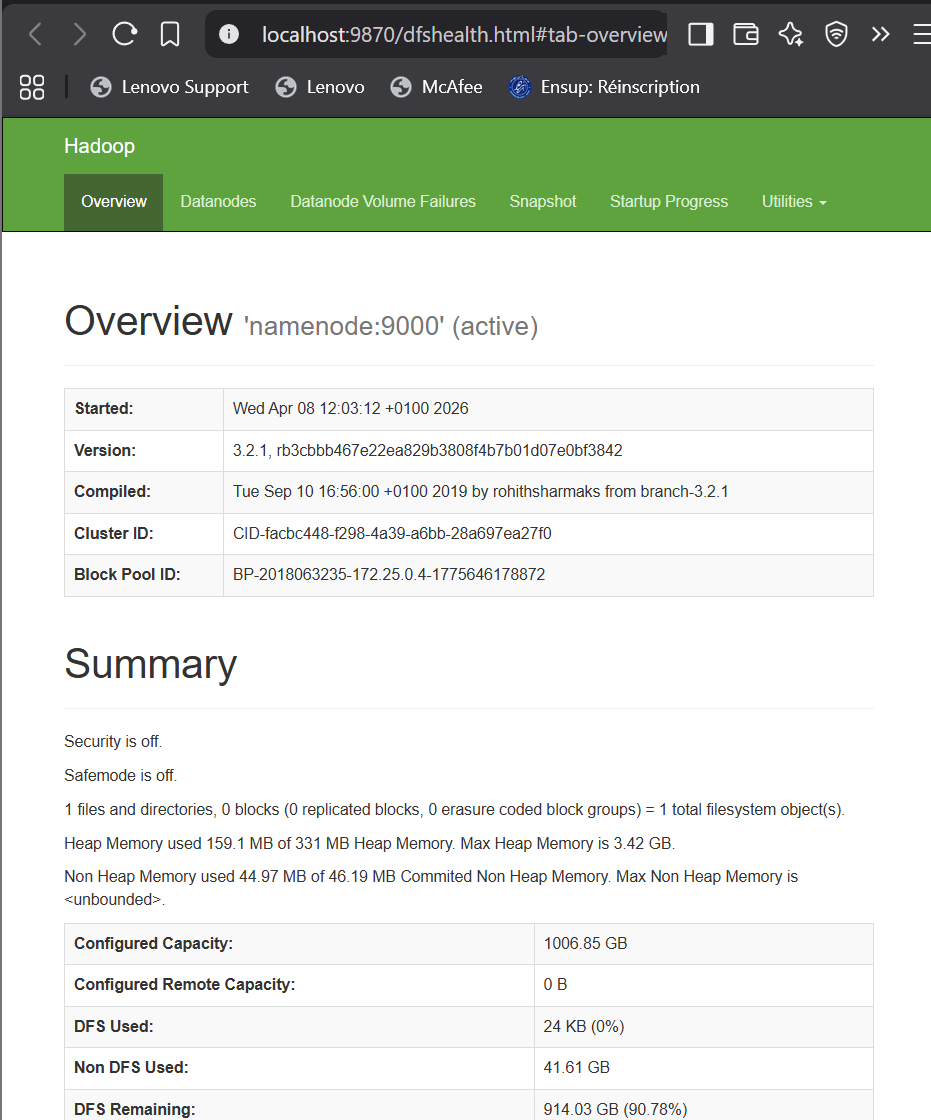
\includegraphics[width=0.7\textwidth]{figures/batch/hdfsUI1.png}
    \caption{HDFS Web interface showing the NameNode status and the availability of the distributed file system.}
    \label{fig:hdfs-ui-namenode}
\end{figure}

\section{HDFS Organization}

\subsection{Raw Partitions}

HDFS is used as durable storage for the raw logs \cite{hdfs_docs}. The project adopts a monthly partitioning convention under the \texttt{/logs} directory. The \texttt{/logs/year=2024/month=XX} area therefore corresponds to the raw input of the batch layer and the Kafka replay. It should not be confused with \texttt{/data/cybersecurity/batch}, which contains the analytical outputs.

Each month of the year 2024 has a \texttt{data.csv} file, for example:

\begin{itemize}
    \item \texttt{/logs/year=2024/month=01/data.csv}
    \item \texttt{/logs/year=2024/month=02/data.csv}
    \item \texttt{/logs/year=2024/month=12/data.csv}
\end{itemize}

This structure allows Spark batch jobs to read all months with the pattern \texttt{/logs/year=2024/month=*/data.csv}. It also allows the Kafka producer to replay the same partitions in the speed layer. The HDFS partitions therefore act as the source of truth: if an HBase or Cassandra table must be rebuilt, the computations can restart from the same monthly files.

The command below lists the monthly partitions under \texttt{/logs/year=2024}. This verification shows that the raw logs are organized by month, which makes it possible to process the full year or replay a specific period.

\begin{cmdbox}
docker exec -it namenode bash\\
hdfs dfs -ls /logs/year=2024
\end{cmdbox}

\begin{figure}[H]
    \centering
    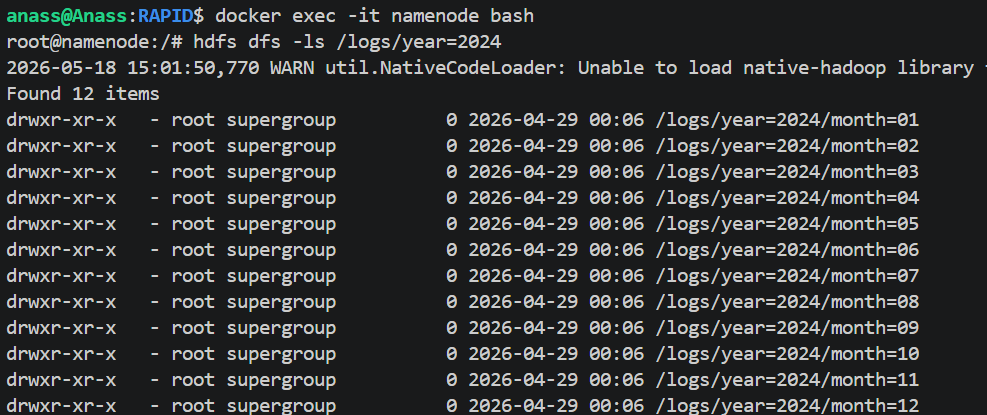
\includegraphics[width=\textwidth]{figures/batch/hdfspartition.png}
    \caption{Partitioning of raw logs in HDFS by year and month.}
    \label{fig:hdfs-raw-partitioning}
\end{figure}

\subsection{Batch Outputs}

Historical outputs are written under \texttt{/data/cybersecurity/batch}. The Spark scripts in \texttt{spark/batch/} generally write two forms of output: a Parquet output in HDFS for audit and reconstruction, then an HBase table for serving the aggregated views. Table~\ref{tab:hdfs-batch-outputs} summarizes the paths observed in the project.

\begingroup
\footnotesize
\setlength{\tabcolsep}{5pt}
\renewcommand{\arraystretch}{1.32}
\begin{longtable}{|
    >{\raggedright\arraybackslash\bfseries}p{0.24\textwidth}|
    >{\raggedright\arraybackslash}p{0.34\textwidth}|
    >{\raggedright\arraybackslash}p{0.30\textwidth}|
}
    \caption{Batch outputs produced in HDFS.}
    \label{tab:hdfs-batch-outputs}\\
    \hline
    \tablehead{Spark Job} & \tablehead{HDFS Path} & \tablehead{Role of the Result} \\
    \hline
    \endfirsthead
    \hline
    \tablehead{Spark Job} & \tablehead{HDFS Path} & \tablehead{Role of the Result} \\
    \hline
    \endhead
    \batchcell{\scriptcell{top10\_malicious\_ips.py}} &
    \batchcell{\texttt{/data/cybersecurity/}\\\texttt{batch/top10\_malicious\_ips}} &
    Ranking of the most dangerous source IPs and basis for the historical reputation score. \\
    \hline

    \batchcell{\scriptcell{attack\_path\_analysis.py}} &
    \batchcell{\texttt{/data/cybersecurity/}\\\texttt{batch/attack\_patterns}} &
    Aggregation of SQLi, XSS, Path Traversal and ToolScan patterns by attack type and threat label. \\
    \hline

    \batchcell{\scriptcell{hbase\_threat\_timeline.py}} &
    \batchcell{\texttt{/data/cybersecurity/}\\\texttt{batch/threat\_timeline/}\\\texttt{hourly}\\\texttt{/data/cybersecurity/}\\\texttt{batch/threat\_timeline/}\\\texttt{daily}} &
    Hourly and daily event time series by threat level. \\
    \hline

    \batchcell{\scriptcell{port\_scan\_detection.py}} &
    \batchcell{\texttt{/data/cybersecurity/}\\\texttt{batch/port\_scans}} &
    Five-minute windows in which a source IP contacts more than twenty distinct ports. \\
    \hline

    \batchcell{\scriptcell{volume\_by\_threat.py}} &
    \batchcell{\texttt{/data/cybersecurity/}\\\texttt{batch/volume\_by\_threat}} &
    Network volume statistics by \texttt{threat\_label}, including mean, maximum, standard deviation and 95th percentile. \\
    \hline

    \batchcell{\scriptcell{multistep\_attack\_detection.py}} &
    \batchcell{\texttt{/data/cybersecurity/}\\\texttt{batch/views/}\\\texttt{multistep\_attacks}} &
    Enriched view of IPs that combine reconnaissance, SQLi exploitation and Path Traversal. \\
    \hline

    Intermediate view &
    \batchcell{\texttt{/data/cybersecurity/}\\\texttt{batch/classified\_attacks}} &
    Parquet input expected by the multi-step detector to group already classified attacks. \\
    \hline
\end{longtable}
\endgroup

This organization clearly separates raw files, analytical outputs, and serving-ready views. Parquet files do not replace HBase: they serve as a technical trace and as support for recomputation. HBase receives only the aggregations required for fast reads.

The following commands show the global \texttt{/data/cybersecurity} directory and then the batch output folders. The result validates the presence of views generated by Spark, including \texttt{attack\_patterns}, \texttt{port\_scans}, \texttt{threat\_timeline}, \texttt{top\_malicious\_ips}, \texttt{views} and \texttt{volume\_by\_threat}.

\begin{cmdbox}
hdfs dfs -ls /data/cybersecurity\\
hdfs dfs -ls /data/cybersecurity/batch
\end{cmdbox}

\begin{figure}[H]
    \centering
    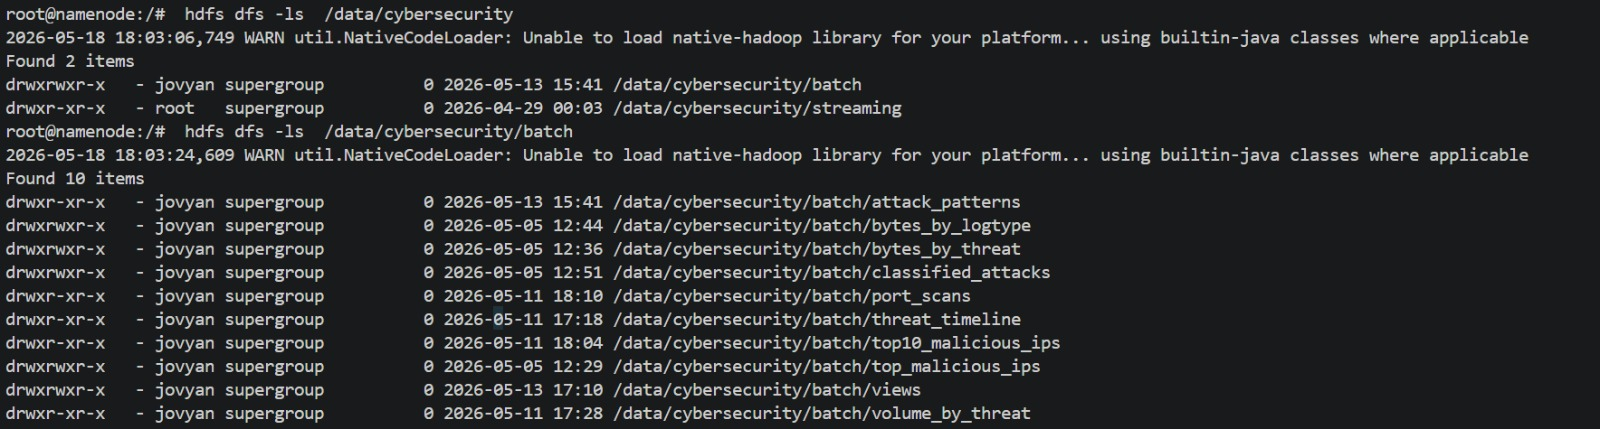
\includegraphics[width=\textwidth]{figures/batch/spark_batch_output_folders_and_directory_structure.jpeg}
    \caption{HDFS directories containing the outputs generated by Spark batch processing.}
    \label{fig:spark-batch-output-folders}
\end{figure}

\subsection{HDFS Storage Zones}

The separation of HDFS zones clarifies the role of each directory. The \texttt{/logs/year=2024/month=XX} zone corresponds to raw inputs, while \texttt{/data/cybersecurity/batch} corresponds to analytical results. The \texttt{/data/cybersecurity/streaming} zone may exist in the tree, but it is not the main scope of this chapter.

\begingroup
\footnotesize
\setlength{\tabcolsep}{5pt}
\renewcommand{\arraystretch}{1.28}
\begin{longtable}{|
    >{\raggedright\arraybackslash\bfseries}p{0.33\textwidth}|
    >{\raggedright\arraybackslash}p{0.24\textwidth}|
    >{\raggedright\arraybackslash}p{0.31\textwidth}|
}
    \caption{HDFS zones used by the batch layer.}
    \label{tab:hdfs-storage-zones}\\
    \hline
    \tablehead{HDFS Zone} & \tablehead{Content} & \tablehead{Usage} \\
    \hline
    \endfirsthead
    \hline
    \tablehead{HDFS Zone} & \tablehead{Content} & \tablehead{Usage} \\
    \hline
    \endhead
    \batchcell{\texttt{/logs/year=2024/}\\\texttt{month=XX}} &
    Partitioned raw logs &
    Batch source and Kafka replay \\
    \hline

    \batchcell{\texttt{/data/cybersecurity/}\\\texttt{batch}} &
    Parquet outputs &
    Audit, verification and reconstruction \\
    \hline

    \batchcell{\texttt{/data/cybersecurity/}\\\texttt{batch/views}} &
    Analytical views &
    Results prepared for exploitation \\
    \hline

    \batchcell{\texttt{/data/cybersecurity/}\\\texttt{streaming}} &
    Possible streaming outputs &
    Outside the main scope of the batch chapter \\
    \hline
\end{longtable}
\endgroup

\section{Batch Job Input Schema}

Batch jobs use an explicit schema to avoid automatic inference and maintain a stable data contract with HDFS. This contract is consistent with the architecture chapter: the same attributes feed batch processing, Kafka replay, and serving views.

\begingroup
\small
\setlength{\tabcolsep}{5pt}
\renewcommand{\arraystretch}{1.28}
\begin{longtable}{|
    >{\raggedright\arraybackslash\bfseries}p{0.24\textwidth}|
    >{\raggedright\arraybackslash}p{0.64\textwidth}|
}
    \caption{Input schema of batch processing.}
    \label{tab:batch-input-schema}\\
    \hline
    \tablehead{Field} & \tablehead{Analytical Role} \\
    \hline
    \endfirsthead
    \hline
    \tablehead{Field} & \tablehead{Analytical Role} \\
    \hline
    \endhead
    \texttt{timestamp} & Event time, used for windows and historical series. \\
    \hline
    \texttt{source\_ip} & Source address used for reputation, scans and correlations. \\
    \hline
    \texttt{dest\_ip} & Network target observed in the log. \\
    \hline
    \texttt{protocol} & Network protocol, useful for filtering certain behaviors such as TCP scans. \\
    \hline
    \texttt{action} & Observed action, for example an allowed or blocked request. \\
    \hline
    \texttt{threat\_label} & Threat class used for historical aggregations. \\
    \hline
    \texttt{log\_type} & Log category, useful for qualifying the source of the event. \\
    \hline
    \scriptcell{bytes\_transferred} & Network volume used in traffic statistics. \\
    \hline
    \texttt{user\_agent} & Field used to detect ToolScan and certain offensive tool signatures. \\
    \hline
    \texttt{request\_path} & HTTP path used to detect SQLi, XSS and Path Traversal. \\
    \hline
\end{longtable}
\endgroup

Spark reads HDFS partitions with an \textit{HDFS-first} strategy. If HDFS is unavailable during a development run, the scripts provide a local fallback to the local path \texttt{/home/jovyan/work/batch/}\linebreak[1]\texttt{cybersecurity\_threat\_detection\_logs.csv}. In the RAPID deployment, however, the HDFS path remains the nominal path, because it makes it possible to process the full year and rebuild outputs reproducibly \cite{spark_docs}.

\subsection{Spark Batch Scripts and Responsibilities}

The scripts in the \texttt{spark/batch/} folder materialize the analytical logic of the batch layer. Each script reads the historical logs, builds a specialized view, and then writes the result either as Parquet in HDFS or into HBase when the view must be consumed quickly by the service. This dual output provides technical traceability: HDFS makes it possible to verify and rebuild computations, while HBase exposes the results as directly queryable rows.

The \texttt{ml\_bonus.py} script is treated as an experimental complement: it locally trains a Random Forest model on simple features and saves local predictions. It is therefore not central to HBase serving, unlike the scripts that feed the \texttt{ip\_reputation}, \texttt{attack\_patterns}, \texttt{threat\_timeline}, \texttt{port\_scans}, \texttt{threat\_volume} and \texttt{multistep\_attacks} tables.

\begingroup
\scriptsize
\setlength{\tabcolsep}{4pt}
\renewcommand{\arraystretch}{1.34}
\begin{longtable}{|
    >{\raggedright\arraybackslash\bfseries}p{0.23\textwidth}|
    >{\raggedright\arraybackslash}p{0.42\textwidth}|
    >{\raggedright\arraybackslash}p{0.25\textwidth}|
}
    \caption{Summary of Spark batch scripts and produced views.}
    \label{tab:spark-batch-scripts}\\
    \hline
    \tablehead{Script} & \tablehead{Processing Performed} & \tablehead{HDFS Output / HBase Table} \\
    \hline
    \endfirsthead
    \hline
    \tablehead{Script} & \tablehead{Processing Performed} & \tablehead{HDFS Output / HBase Table} \\
    \hline
    \endhead

    \batchcell{\scriptcell{top10\_malicious\_ips.py}} &
    Ranks source IPs whose \texttt{threat\_label} is \texttt{suspicious} or \texttt{malicious}. The script adds SQLi, XSS, Path Traversal and ToolScan indicators, then computes a \texttt{reputation\_score} normalized between 0 and 100. &
    \batchcell{\texttt{batch/top10\_}\\\texttt{malicious\_ips}\\[1mm]\texttt{ip\_reputation}} \\
    \hline

    \batchcell{\scriptcell{attack\_path\_analysis.py}} &
    Analyzes \texttt{request\_path} and \texttt{user\_agent} with SQLi, XSS, Path Traversal and ToolScan signatures. It aggregates occurrences, volumes, distinct IPs and the latest observation by attack type and threat level. &
    \batchcell{\texttt{batch/attack\_}\\\texttt{patterns}\\[1mm]\texttt{attack\_patterns}} \\
    \hline

    \batchcell{\scriptcell{hbase\_threat\_timeline.py}} &
    Produces an hourly and daily historical timeline. The aggregates store the number of events, the number of distinct IPs and the total volume by \texttt{threat\_label}. &
    \batchcell{\texttt{batch/threat\_}\\\texttt{timeline/hourly}\\\texttt{batch/threat\_}\\\texttt{timeline/daily}\\[1mm]\texttt{threat\_timeline}} \\
    \hline

    \batchcell{\scriptcell{port\_scan\_detection.py}} &
    Filters TCP logs, extracts the destination port and detects sources that contact more than twenty distinct ports within a five-minute window. &
    \batchcell{\texttt{batch/port\_scans}\\[1mm]\texttt{port\_scans}} \\
    \hline

    \batchcell{\scriptcell{volume\_by\_threat.py}} &
    Correlates \texttt{bytes\_transferred} with \texttt{threat\_label}. The script computes the number of events, the mean, minimum, maximum and total volumes, the standard deviation and the 95th percentile. &
    \batchcell{\texttt{batch/volume\_}\\\texttt{by\_threat}\\[1mm]\texttt{threat\_volume}} \\
    \hline

    \batchcell{\scriptcell{multistep\_attack\_detection.py}} &
    Reads the \texttt{classified\_attacks} view and searches for IPs that combine ToolScan, SQLi and Path Traversal. It enriches each IP with counters, average volume, the number of malicious events and a \texttt{risk\_level}. &
    \batchcell{\texttt{batch/views/}\\\texttt{multistep\_attacks}\\[1mm]\texttt{multistep\_attacks}} \\
    \hline

    \batchcell{\texttt{ml\_bonus.py}} &
    Local bonus script. It trains a Random Forest on \texttt{bytes\_transferred}, \texttt{protocol}, \texttt{action} and \texttt{log\_type}, evaluates accuracy, F1, precision and recall, then saves the predictions. &
    \batchcell{\texttt{./data/}\\\texttt{predictions.parquet}\\[1mm]No HBase table} \\
    \hline
\end{longtable}
\endgroup

\section{Historical Serving with HBase}

\subsection{Modeling Principle}

HBase is used as a historical serving store because its model based on rows, column families and sortable keys is suitable for reads by identifier or by temporal prefix \cite{hbase_docs}. Batch jobs connect to Chawi's Thrift service with HappyBase and write the results into HBase tables. The operational contract observed in the batch scripts uses the \texttt{cf} column family; the column qualifiers then carry the metrics computed by each job.

The HBase list verifies that the serving tables exist before the API or the dashboard queries them. This output illustrates the historical tables used by the batch layer: \texttt{attack\_patterns}, \texttt{ip\_reputation}, \texttt{multistep\_attacks}, \texttt{port\_scans}, \texttt{threat\_timeline} and \texttt{threat\_volume}.

\begin{cmdbox}
docker exec -it hbase hbase shell\\
list
\end{cmdbox}

\begin{figure}[H]
    \centering
    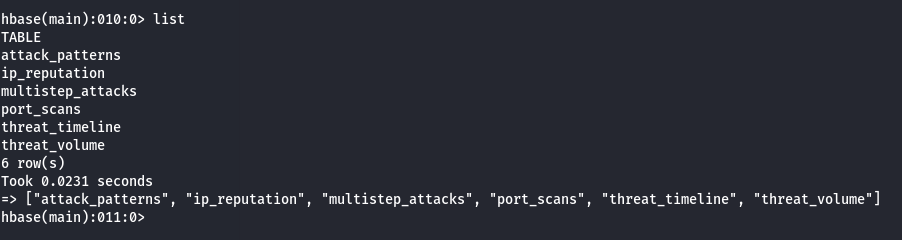
\includegraphics[width=\textwidth]{figures/batch/hbase_tables_list.png}
    \caption{List of HBase tables used to serve historical batch results.}
    \label{fig:hbase-tables-list}
\end{figure}

The HBase creation script initializes the main IP reputation, attack pattern and threat timeline tables. The batch scripts present in the project also add specialized tables for port scans, traffic volumes and multi-step attacks. These tables are documented here because they belong to the same batch/HBase contract found in the repository.

\subsection{HBase Modeling Choices}

HBase is not used to store raw logs. The complete logs remain in HDFS, while HBase contains aggregated views ready to be served. This choice reduces the volume read by the API and makes responses more direct for the dashboard.

The row key is chosen according to the expected query pattern: \texttt{source\_ip} for reputation, \texttt{HOURLY|heure|threat\_label} or \texttt{DAILY|jour|threat\_label} for the timeline, \texttt{source\_ip|window\_start} for port scans, and \texttt{THREAT\_VOL|threat\_label} for volume statistics. The \texttt{cf} column family groups the metrics computed by Spark, keeping the model simple and consistent across tables.

\subsection{HBase Tables of the Batch Layer}

Table~\ref{tab:hbase-batch-schemas} details the HBase schemas used to serve historical results. Row keys are chosen to match expected access patterns: an IP for reputation, an attack type for patterns, a temporal prefix for series, or an observation window for port scans.

\begingroup
\scriptsize
\setlength{\tabcolsep}{4pt}
\renewcommand{\arraystretch}{1.34}
\begin{longtable}{|
    >{\raggedright\arraybackslash\bfseries}p{0.15\textwidth}|
    >{\raggedright\arraybackslash}p{0.24\textwidth}|
    >{\raggedright\arraybackslash}p{0.39\textwidth}|
}
    \caption{HBase schemas of batch views.}
    \label{tab:hbase-batch-schemas}\\
    \hline
    \tablehead{Table} & \tablehead{Row Key and Producer} & \tablehead{Main Columns} \\
    \hline
    \endfirsthead
    \hline
    \tablehead{Table} & \tablehead{Row Key and Producer} & \tablehead{Main Columns} \\
    \hline
    \endhead

    \texttt{ip\_reputation} &
    \batchcell{\texttt{source\_ip}\\\texttt{top10\_malicious\_ips.py}} &
    \batchcell{\texttt{cf:threat\_count}, \texttt{cf:sqli\_hits}, \texttt{cf:xss\_hits},\\
    \texttt{cf:traversal\_hits}, \texttt{cf:tool\_hits}, \texttt{cf:avg\_bytes},\\
    \texttt{cf:reputation\_score}} \\
    \hline

    \batchcell{\texttt{attack\_}\\\texttt{patterns}} &
    \batchcell{\texttt{attack\_type|}\\\texttt{threat\_label}\\\texttt{attack\_path\_}\\\texttt{analysis.py}} &
    \batchcell{\texttt{cf:attack\_type}, \texttt{cf:threat\_label}, \texttt{cf:occurrences},\\
    \texttt{cf:avg\_bytes}, \texttt{cf:total\_bytes}, \texttt{cf:distinct\_ips},\\
    \texttt{cf:last\_seen}} \\
    \hline

    \batchcell{\texttt{threat\_}\\\texttt{timeline}} &
    \batchcell{\texttt{HOURLY|heure|}\\\texttt{threat\_label}\\\texttt{DAILY|jour|}\\\texttt{threat\_label}\\\texttt{hbase\_threat\_}\\\texttt{timeline.py}} &
    \batchcell{\texttt{cf:heure} or \texttt{cf:jour}, \texttt{cf:threat\_label},\\
    \texttt{cf:event\_count}, \texttt{cf:distinct\_ips}, \texttt{cf:total\_bytes}} \\
    \hline

    \texttt{port\_scans} &
    \batchcell{\texttt{source\_ip|}\\\texttt{window\_start}\\\texttt{port\_scan\_detection.py}} &
    \batchcell{\texttt{cf:source\_ip}, \texttt{cf:distinct\_ports},\\
    \texttt{cf:total\_connections}, \texttt{cf:window\_start}, \texttt{cf:window\_end}} \\
    \hline

    \texttt{threat\_volume} &
    \batchcell{\texttt{THREAT\_VOL|}\\\texttt{threat\_label}\\\texttt{volume\_by\_threat.py}} &
    \batchcell{\texttt{cf:threat\_label}, \texttt{cf:total\_bytes}, \texttt{cf:avg\_bytes},\\
    \texttt{cf:min\_bytes}, \texttt{cf:max\_bytes}, \texttt{cf:stddev\_bytes},\\
    \texttt{cf:p95\_bytes}, \texttt{cf:count}} \\
    \hline

    \batchcell{\texttt{multistep\_}\\\texttt{attacks}} &
    \batchcell{\texttt{source\_ip}\\\scriptcell{multistep\_attack\_detection.py}} &
    \batchcell{\texttt{cf:total\_events}, \texttt{cf:attack\_types}, \texttt{cf:sqli\_hits},\\
    \texttt{cf:traversal\_hits}, \texttt{cf:tool\_hits}, \texttt{cf:avg\_bytes},\\
    \texttt{cf:malicious\_count}, \texttt{cf:risk\_level}} \\
    \hline
\end{longtable}
\endgroup

\begingroup
\small
\setlength{\tabcolsep}{5pt}
\renewcommand{\arraystretch}{1.28}
\begin{longtable}{|
    >{\raggedright\arraybackslash\bfseries}p{0.29\textwidth}|
    >{\raggedright\arraybackslash}p{0.59\textwidth}|
}
    \caption{API/dashboard usage of batch views.}
    \label{tab:hbase-frontend-usage}\\
    \hline
    \tablehead{HBase Table} & \tablehead{Service/dashboard Usage} \\
    \hline
    \endfirsthead
    \hline
    \tablehead{HBase Table} & \tablehead{Service/dashboard Usage} \\
    \hline
    \endhead
    \texttt{ip\_reputation} & Historical score and reputation detail by IP. \\
    \hline
    \texttt{attack\_patterns} & Distribution of detected attack families. \\
    \hline
    \texttt{threat\_timeline} & Chronological threat chart. \\
    \hline
    \texttt{port\_scans} & Detected scan behaviors. \\
    \hline
    \texttt{threat\_volume} & Volume chart and statistics by threat level. \\
    \hline
    \texttt{multistep\_attacks} & Advanced multi-step correlation view. \\
    \hline
\end{longtable}
\endgroup

\subsection{\texttt{ip\_reputation}}

The \texttt{ip\_reputation} table is the historical view most directly used by the service. Each row represents a source IP and groups the signals observed across the complete history: average volume, reputation score, SQLi, XSS and Path Traversal indicators, offensive tools and number of threatening events. The expected query is a direct read by \texttt{source\_ip}.

The HBase command below verifies the table schema and displays a sample of served rows. It shows that historical reputation is materialized by IP with \texttt{avg\_bytes}, \texttt{reputation\_score}, \texttt{sqli\_hits}, \texttt{threat\_count}, \texttt{tool\_hits}, \texttt{traversal\_hits} and \texttt{xss\_hits}.

\begin{cmdbox}
describe 'ip\_reputation'\\
scan 'ip\_reputation', \{LIMIT =\textgreater{} 5\}
\end{cmdbox}

\begin{figure}[H]
    \centering
    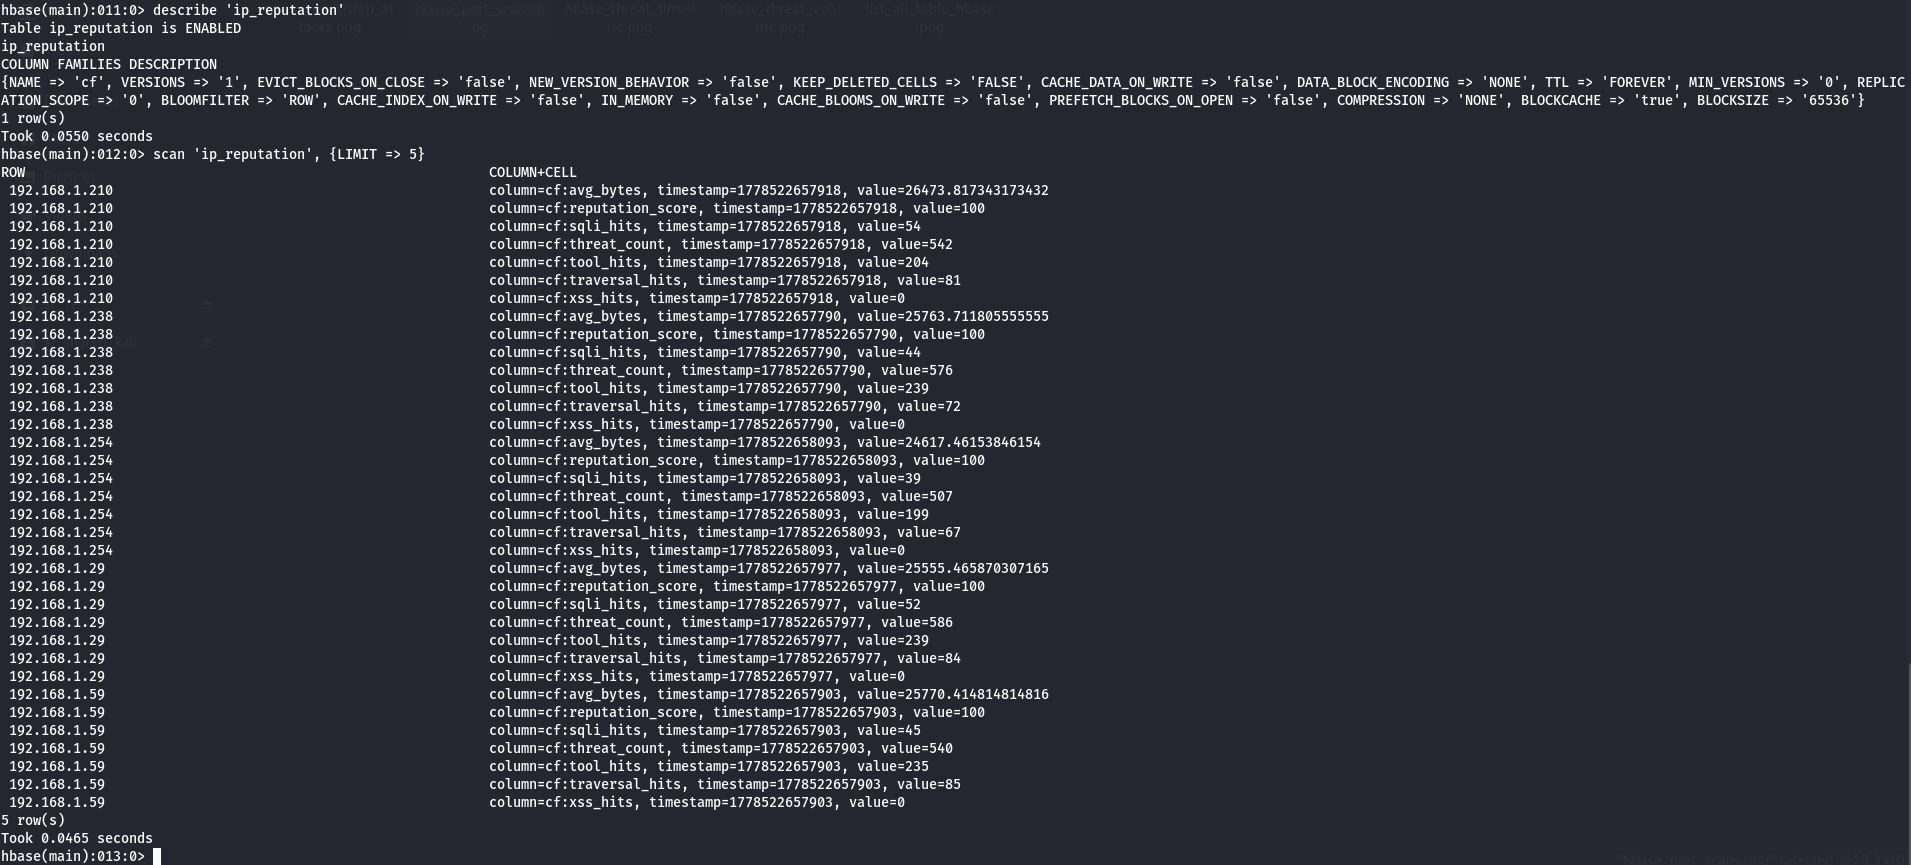
\includegraphics[width=\textwidth]{figures/batch/hbase_ip_reputation.png}
    \caption{Schema and sample rows of the HBase \texttt{ip\_reputation} table.}
    \label{fig:hbase-ip-reputation}
\end{figure}

This table allows the API to complement the real-time state with historical memory. When a client requests \texttt{/threats/ip/<ip>}, the API reads the HBase row associated with the IP and compares this historical signal with Cassandra scores in order to produce a single decision for the dashboard.

\subsection{\texttt{attack\_patterns}}

The \texttt{attack\_patterns} table stores the attack patterns extracted from HTTP paths and user agents. The path analysis job classifies events with regular expressions for SQLi, XSS, Path Traversal and ToolScan. The composite key associates the attack type with the threat level, making each combination directly addressable and avoiding an overly wide row per attack type. The expected read is by attack family and by \texttt{threat\_label} to build an aggregated distribution.

The \texttt{cf:occurrences}, \texttt{cf:distinct\_ips}, \texttt{cf:total\_bytes}, \texttt{cf:avg\_bytes} and \texttt{cf:last\_seen} columns provide a synthetic view of historical behavior. This modeling is useful for explaining which attack families dominate the corpus and for feeding aggregated visualizations without rereading all HDFS files.

\subsection{\texttt{threat\_timeline}}

The \texttt{threat\_timeline} table serves temporal trends. The HBase timeline job produces an hourly and daily historical evolution, separated by \texttt{threat\_label}. The expected read is by period and by threat label in order to feed a temporal chart.

The following commands verify the table schema and display sample rows. This verification shows that the table stores the daily evolution by label with \texttt{event\_count}, \texttt{distinct\_ips}, \texttt{total\_bytes}, \texttt{jour} and \texttt{threat\_label}.

\begin{cmdbox}
describe 'threat\_timeline'\\
scan 'threat\_timeline', \{LIMIT =\textgreater{} 5\}
\end{cmdbox}

\begin{figure}[H]
    \centering
    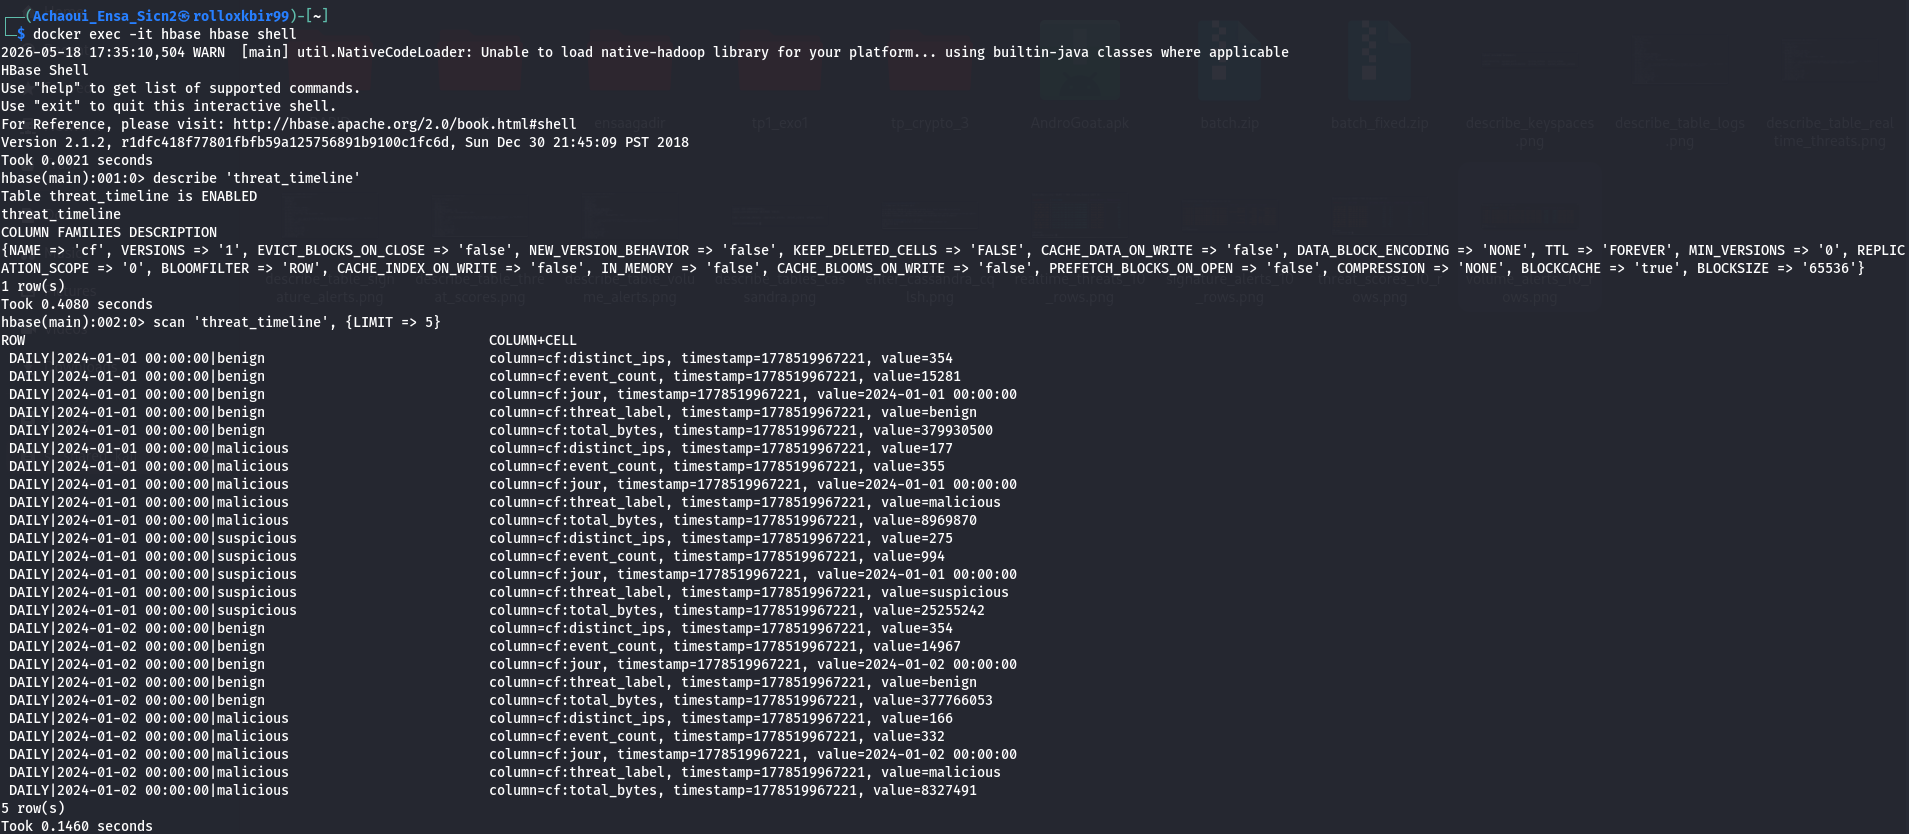
\includegraphics[width=\textwidth]{figures/batch/hbase_threat_timeline.png}
    \caption{Schema and sample rows of the HBase \texttt{threat\_timeline} table.}
    \label{fig:hbase-threat-timeline}
\end{figure}

\subsection{\texttt{port\_scans}}

The \texttt{port\_scans} table stores the windows where a TCP source contacts a high number of distinct ports. Each row associates a source IP with a time window and stores the counters required to directly serve port scan detection results. The expected read is by \texttt{source\_ip} and \texttt{window\_start}.

The HBase output confirms that scan aggregations are materialized. It exposes the \texttt{source\_ip}, \texttt{distinct\_ports}, \texttt{total\_connections}, \texttt{window\_start} and \texttt{window\_end} columns.

\begin{cmdbox}
describe 'port\_scans'\\
scan 'port\_scans', \{LIMIT =\textgreater{} 5\}
\end{cmdbox}

\begin{figure}[H]
    \centering
    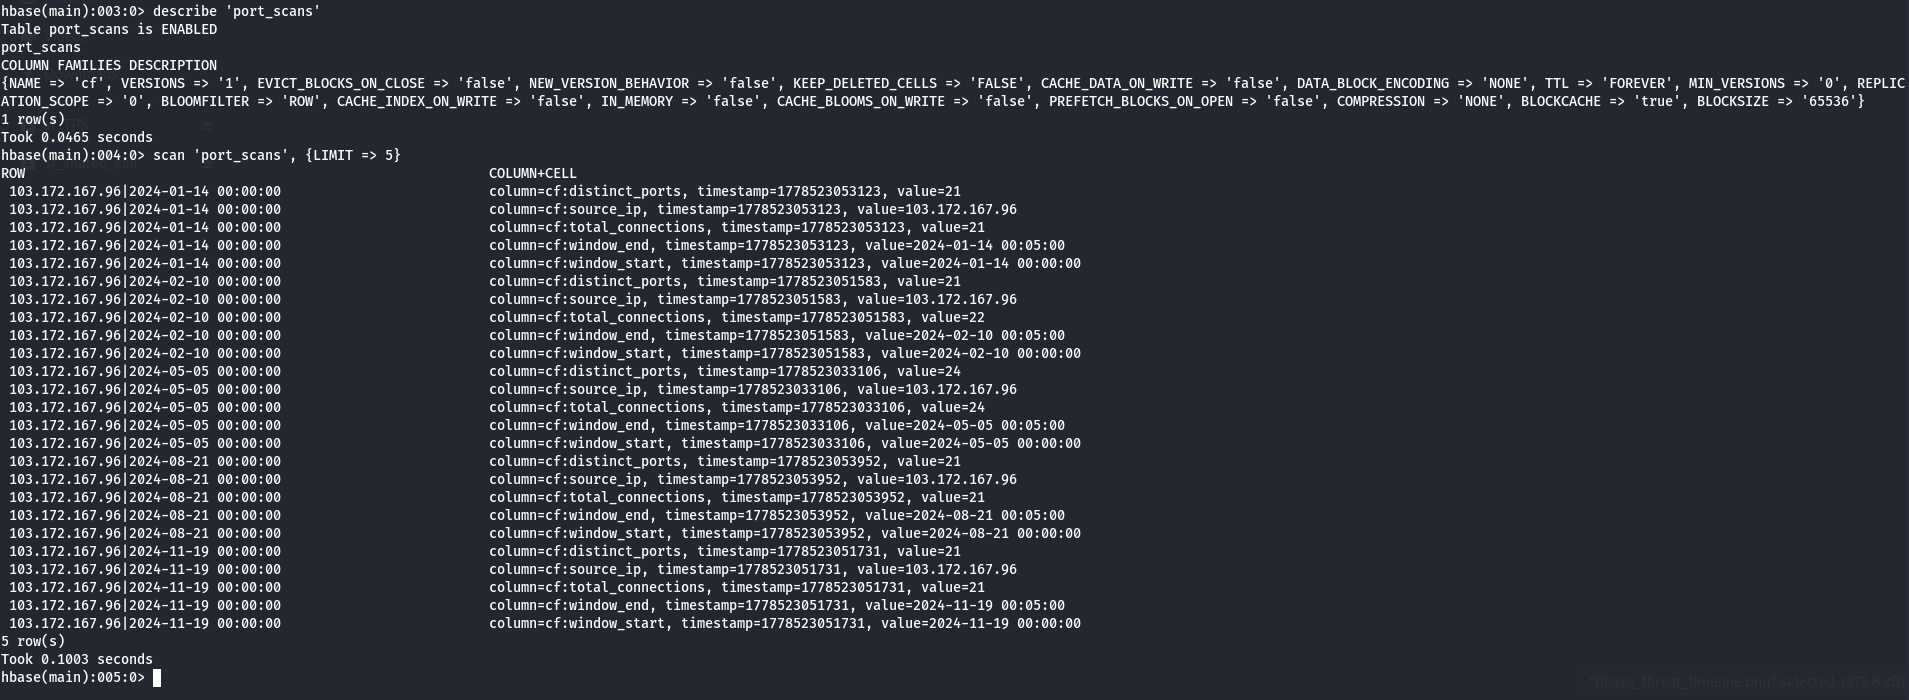
\includegraphics[width=\textwidth]{figures/batch/hbase_port_scans.png}
    \caption{Schema and sample rows of the HBase \texttt{port\_scans} table.}
    \label{fig:hbase-port-scans}
\end{figure}

\subsection{\texttt{threat\_volume}}

The \texttt{threat\_volume} table aggregates transferred bytes by threat level and highlights high-volume behaviors, notably with the 95th percentile. The expected read is by \texttt{threat\_label} in order to compare traffic volumes across threat classes.

The commands below display the schema and a sample of the stored statistics. The table contains the \texttt{avg\_bytes}, \texttt{count}, \texttt{max\_bytes}, \texttt{min\_bytes}, \texttt{p95\_bytes}, \texttt{stddev\_bytes} and \texttt{total\_bytes} aggregates by \texttt{threat\_label}.

\begin{cmdbox}
describe 'threat\_volume'\\
scan 'threat\_volume', \{LIMIT =\textgreater{} 5\}
\end{cmdbox}

\begin{figure}[H]
    \centering
    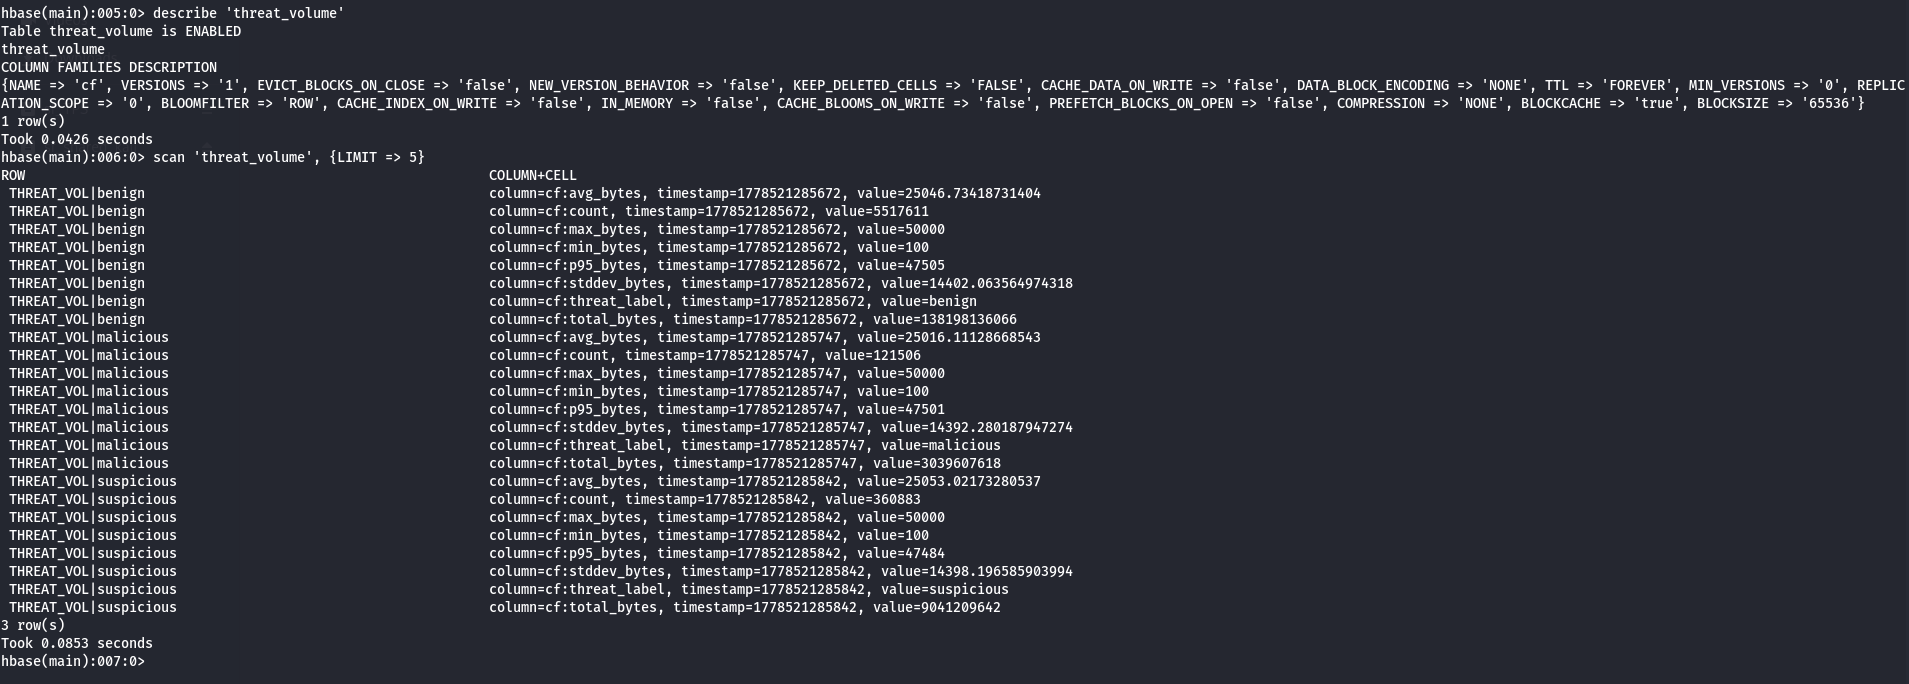
\includegraphics[width=\textwidth]{figures/batch/hbase_threat_volume.png}
    \caption{Schema and sample rows of the HBase \texttt{threat\_volume} table.}
    \label{fig:hbase-threat-volume}
\end{figure}

\subsection{\texttt{multistep\_attacks}}

The \texttt{multistep\_attacks} table is used by the \texttt{multistep\_attack\_detection.py} script. It groups IPs that appear in several stages of an attack chain: tool-based reconnaissance, SQLi exploitation and Path Traversal. The expected read is by \texttt{source\_ip} in order to identify the attack chains associated with an origin.

The obtained result validates the storage of multi-step correlations for serving. It shows columns such as \texttt{attack\_types}, \texttt{sqli\_hits}, \texttt{traversal\_hits}, \texttt{tool\_hits}, \texttt{avg\_bytes}, \texttt{malicious\_count} and \texttt{risk\_level}. Some validation screenshots may also display presentation columns such as \texttt{attack\_chain} or \texttt{ordered\_steps}, used to make the chain more readable.

\begin{cmdbox}
describe 'multistep\_attacks'\\
scan 'multistep\_attacks', \{LIMIT =\textgreater{} 5\}
\end{cmdbox}

\begin{figure}[H]
    \centering
    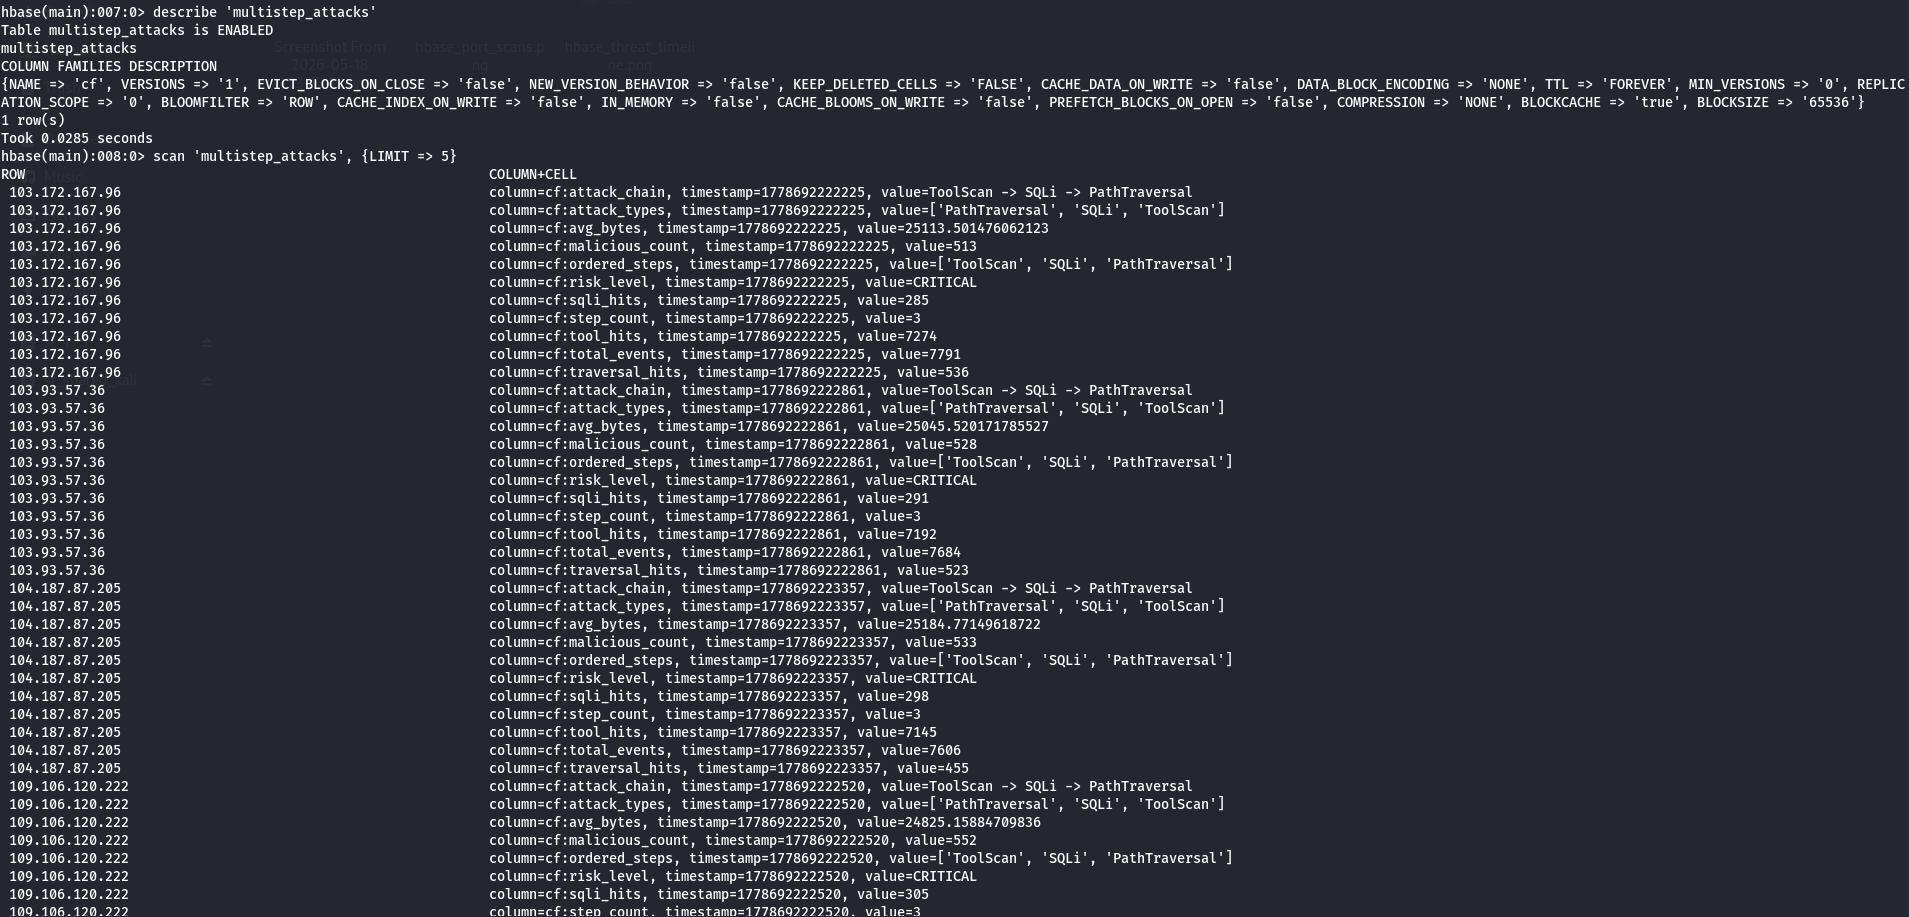
\includegraphics[width=\textwidth]{figures/batch/hbase_multistep_attacks.png}
    \caption{Schema and sample rows of the HBase \texttt{multistep\_attacks} table.}
    \label{fig:hbase-multistep-attacks}
\end{figure}

These tables do not replace \texttt{ip\_reputation}; they add specialized analytical views. They are important within Chawi's storage responsibility because they transform batch results into objects directly readable by a service: an HBase row already represents an analytical decision or a window of interest, rather than a raw event.

\section{Experimental Validation of Screenshots}

The screenshots integrated into this chapter are not decorative: they constitute an experimental validation of the storage chain. The HDFS commands confirm the existence of raw partitions and the presence of Spark batch outputs. The HBase commands validate the creation of serving tables, their schemas and the presence of sample rows. Together, these checks demonstrate that the batch results have moved from rebuildable analytical storage to serving-ready HBase views.

\section{Serving Flow between HDFS, Spark and HBase}

The batch flow follows a stable sequence. First, Spark reads the monthly HDFS partitions from \texttt{/logs/year=2024/month=XX}. Second, the job applies an aggregation or classification: IP reputation, attack patterns, timeline, port scans, volume or multi-step chains. Third, the result is written as Parquet under \texttt{/data/cybersecurity/batch}. Fourth, the metrics useful for serving are inserted into HBase through HappyBase and the Thrift port \texttt{9090}.

This model provides two advantages. On the one hand, HBase tables remain lightweight and read-oriented: they do not contain raw logs, but views prepared for the API. On the other hand, HDFS outputs remain available to verify aggregations, compare two versions of a job, or rebuild an HBase table after a schema change. Chawi therefore ensures the transition between batch analytical results and data ready to be served.

\section{Consistency with the Lambda Architecture}

The design of this batch layer reinforces the overall consistency of RAPID. HDFS guarantees reproducibility, Spark provides distributed computation, and HBase materializes historical views. Cassandra remains the operational store of the speed layer, while HBase preserves the long-term memory produced by complete processing. The API can then merge these two temporalities to provide the dashboard with a single result: recent state, historical reputation, final score and recommendation.

Thus, Chawi's contribution in \texttt{03\_batch\_layer.tex} is centered on storing and serving historical results. The HBase tables are not simple copies of files; they are read schemas designed to quickly expose batch results to the rest of the RAPID platform.

\fussy

\section{Speed Layer}
\label{sec:speed}

\subsection{Kafka Ingestion}

The speed layer uses Kafka as the real-time ingestion backbone. The topic \texttt{cybersecurity-logs} receives JSON log events produced from the historical dataset. The producer uses the source IP as the event key, which keeps related events naturally grouped for downstream analysis. Kafka offsets were checked to confirm that the stream is receiving data.

\begin{figure}[H]
    \centering
    
\includegraphics[width=0.88\textwidth]{\detokenize{figures/Speed Layer- Hamza/kafkatopic.png}}
    \caption{Kafka topic verification for \texttt{cybersecurity-logs}.}
    \label{fig:kafka-topic}
\end{figure}

\subsection{Spark Streaming Detection Rules}

Spark Structured Streaming consumes the Kafka topic, parses JSON messages into a DataFrame, applies detection rules, and writes the results to Cassandra. The implemented real-time rules match the project statement:

\begin{itemize}
    \item \textbf{Brute-force detection:} 5 or more blocked/failed events from the same source IP in about one minute.
    \item \textbf{Signature detection:} suspicious tools and payloads such as \texttt{sqlmap}, \texttt{nikto}, \texttt{nmap}, SQL injection expressions, sensitive paths, and XSS-like strings.
    \item \textbf{Abnormal volume detection:} high bytes transferred by source IP in a 10-second window. The academic target is 10 MB/10 seconds; the experiment also includes a calibrated threshold from observed dataset traffic to generate demonstrable alerts.
    \item \textbf{Threat score:} aggregation by source IP using malicious count, suspicious count, brute-force indicators, signature alerts, and traffic volume.
\end{itemize}

\begin{figure}[H]
    \centering
    
\includegraphics[width=0.90\textwidth]{\detokenize{figures/Speed Layer- Hamza/Screenshot 2026-05-13 194424.png}}
    \caption{Real-time signature detection and Cassandra write path.}
    \label{fig:signature-detection}
\end{figure}

\begin{figure}[H]
    \centering
    
\includegraphics[width=0.82\textwidth]{\detokenize{figures/Speed Layer- Hamza/threat_score.png}}
    \caption{Real-time threat score computation per source IP.}
    \label{fig:threat-score}
\end{figure}

\subsection{Cassandra Active Threat Store}

Cassandra stores the active and recent state of the speed layer. The schema follows the access patterns of the API: recent logs by IP, active threats by IP, signature alerts, volume alerts, and aggregate scores.

\begin{table}[H]
    \centering
    \small
    \caption{Cassandra tables used by the speed layer.}
    \label{tab:cassandra-tables}
    \begin{tabularx}{\textwidth}{>{\ttfamily}p{0.27\textwidth} X}
        \toprule
        Table & Role \\
        \midrule
        logs & Raw or normalized events consumed from Kafka \\
        realtime\_threats & Active threats such as brute-force detections \\
        signature\_alerts & Alerts produced by known signatures and suspicious paths \\
        volume\_alerts & Abnormal transferred-byte windows by source IP \\
        threat\_scores & Aggregated risk score per source IP \\
        \bottomrule
    \end{tabularx}
\end{table}

\begin{figure}[H]
    \centering
    
\includegraphics[width=0.72\textwidth]{\detokenize{figures/Speed Layer- Hamza/Capture Cassandra/describe_tables_cassandra.png}}
    \caption{Cassandra keyspace tables used by Spark Streaming and the API.}
    \label{fig:cassandra-tables}
\end{figure}

\subsection{Speed Layer Assessment}

The speed layer satisfies the real-time requirements because it uses Kafka for continuous ingestion, Spark Streaming for low-latency detection, and Cassandra for recent active threats. It detects at least three threat categories in real time: brute force, signature-based attacks, and abnormal volume. The additional threat score makes the output directly usable by the dashboard and the recommendation API.

\chapter{Serving Layer: API and Dashboard}
\label{chap:serving-layer}

\providecommand{\servingcell}[1]{\begin{minipage}[t]{\linewidth}#1\end{minipage}}
\providecolor{cmdcolor}{RGB}{0,92,160}
\providecommand{\tablehead}[1]{\textcolor{cmdcolor}{\textbf{#1}}}

\section{Role of the Serving Layer}

The serving layer is the user access point of RAPID. Its role is not to recompute the indicators produced by the batch and speed layers. Rather, it makes these results queryable through a Web interface and homogeneous JSON responses. In the project's Lambda Architecture, it therefore connects three elements: the historical views stored in HBase, the real-time results stored in Cassandra, and the HTML/JavaScript dashboard that presents this information to the analyst.

This layer exposes the results through the Flask API hosted at \texttt{http://100.73.216.115:5000}. The frontend does not read HBase or Cassandra directly. It only consumes the REST endpoints defined in the service contract, then transforms JSON responses into summary cards, charts, tables, alert feeds and detail windows. This choice keeps the interface decoupled from internal storage details: the dashboard does not need to know the Cassandra queries, HBase scans, or Spark processing that produced the views.

The serving layer therefore addresses two complementary needs. First, it allows users to consult historical batch views from HBase: IP reputation, attack patterns, threat timeline, volumes, port scans and multi-step attacks. Second, it exposes recent operational results from Cassandra: threat scores, signature alerts, volume alerts, real-time threats, adaptive threshold and attack map. The user obtains a unified view without directly seeing the storage difference between the two temporalities.

\section{Dashboard Architecture}

The \texttt{dashboard/} folder contains a static interface composed of HTML, CSS and JavaScript files. The \texttt{index.html} file automatically redirects to \texttt{batch.html}, making the batch view the current entry page. The real-time view remains available through \texttt{dashboard.html}. Both pages share the same general logic. A top bar displays the RAPID identity, the API connection status, the clock and the refresh indication. A control bar then enables IP address search, polling pause, manual refresh and JSON export. The main content is organized into cards, charts and tables.

The \texttt{batch.html} view is HBase-oriented. It contains tab navigation: \textit{Overview}, \textit{Attack Patterns}, \textit{IP Reputation}, \textit{Port Scans} and \textit{Multi-Step}. The page first presents KPI cards to count attack patterns, flagged IPs, port scans, multi-step chains, threat volumes and available HBase tables. The tabs then provide access to historical charts and detailed tables.

Figure~\ref{fig:batch-dashboard-overview-timeline} illustrates the main batch dashboard view, where the analyst verifies the HBase status, historical indicators and temporal evolution of threats.

\begin{figure}[H]
    \centering
    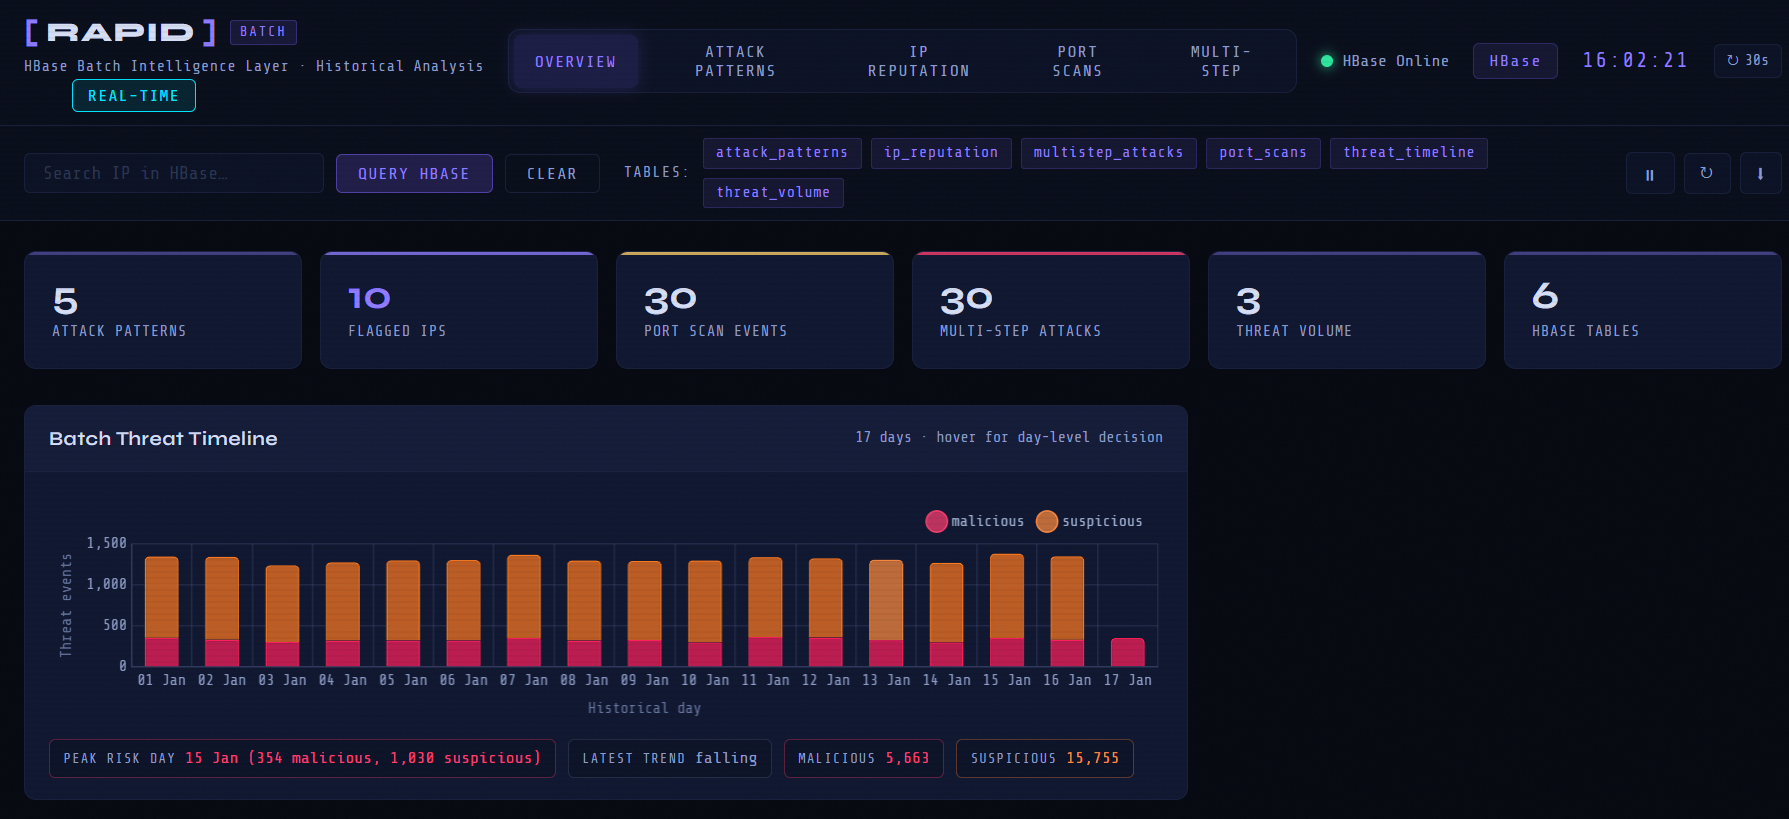
\includegraphics[width=\textwidth]{figures/serving/batch_dashboard/batch_dashboard_overview_timeline.png}
    \caption{General view of the RAPID batch dashboard displaying the HBase status, historical indicators and threat timeline.}
    \label{fig:batch-dashboard-overview-timeline}
\end{figure}

The \texttt{dashboard.html} view is oriented toward the speed layer. It displays real-time scores, volume alerts, signature alerts, a real-time decision queue, an activity timeline and a D3.js attack map. It also contains an IP search modal window that queries the \texttt{/threats/ip/<ip>} endpoint in order to display the score, threat level, recommendation, historical score and associated alerts.

Figure~\ref{fig:speed-dashboard-overview} illustrates the upper part of the real-time view, where the analyst visualizes the main indicators, the maximum score and the distribution of detections.

\begin{figure}[H]
    \centering
    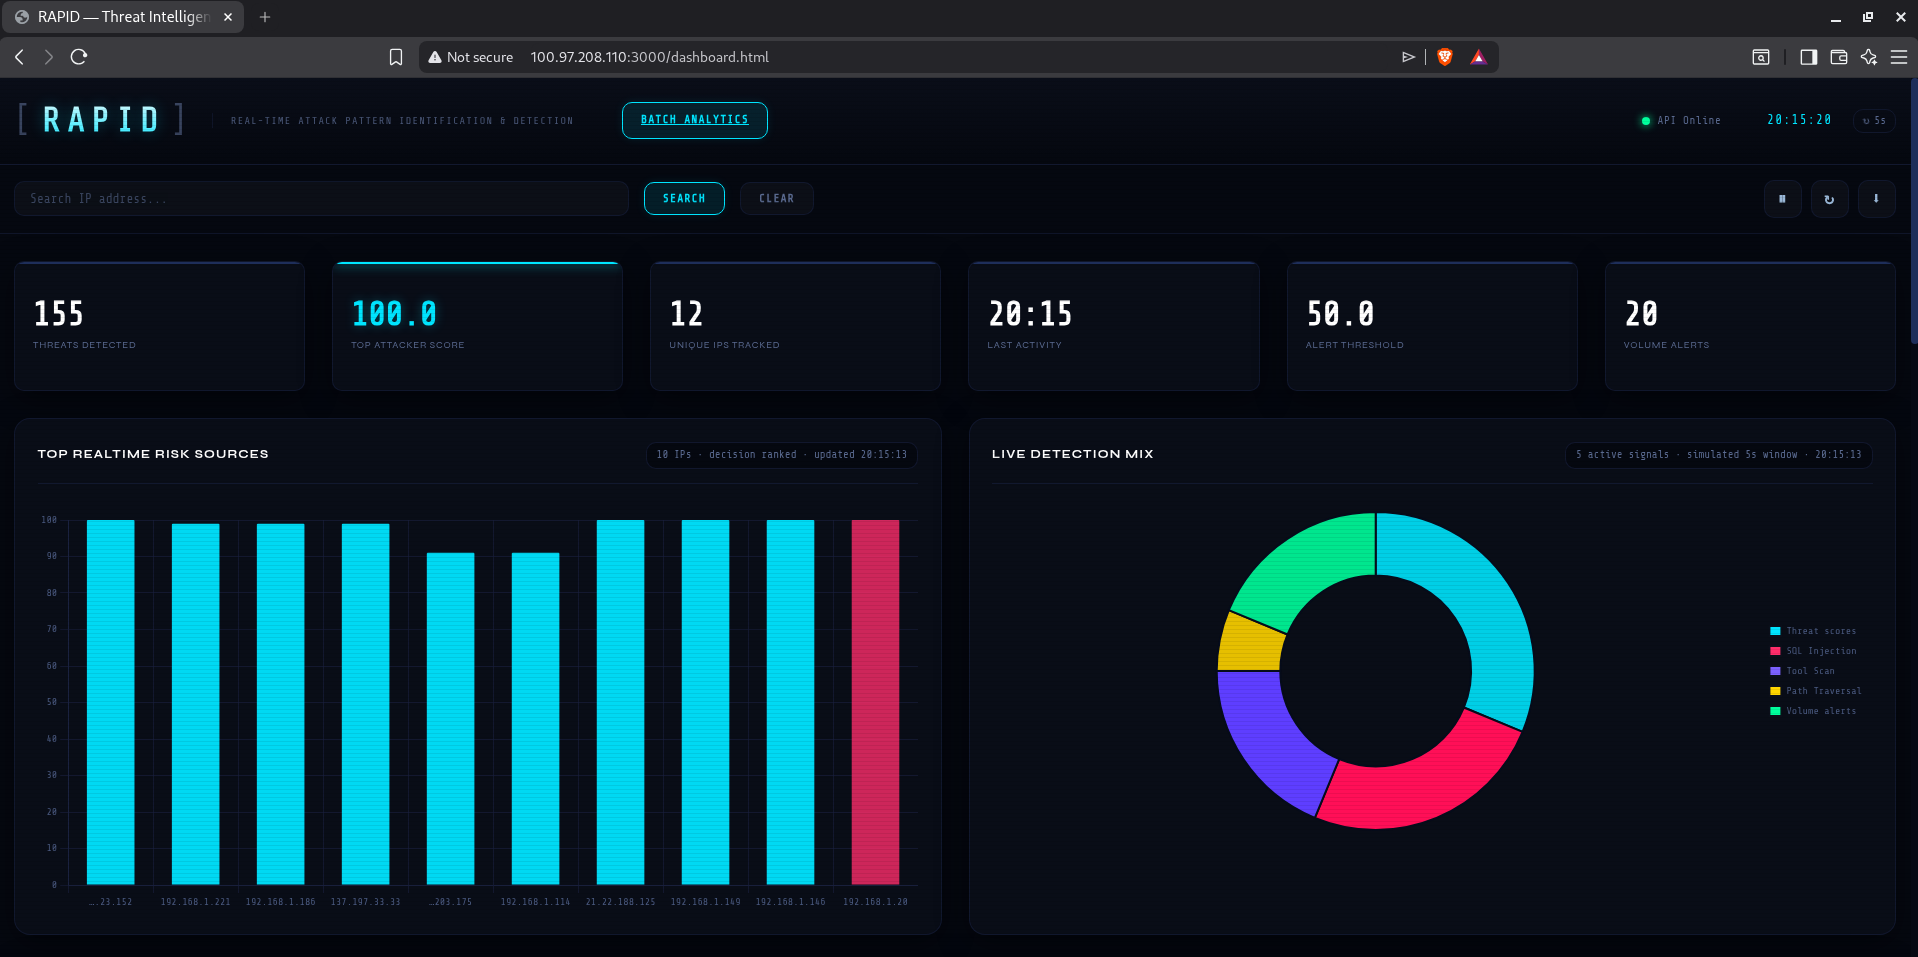
\includegraphics[width=\textwidth]{figures/serving/speed_dashboard/speed_dashboard_overview_top.png}
    \caption{General view of the RAPID real-time dashboard with KPI indicators, the ranking of risky sources and the detection distribution chart.}
    \label{fig:speed-dashboard-overview}
\end{figure}

The dashboard is served as static content. In \texttt{docker/docker-compose.yml}, the \texttt{nginx-dashboard} service uses the \texttt{nginx:alpine} image, mounts \texttt{../dashboard} read-only to \texttt{/usr/share/nginx/html} and publishes port \texttt{3000:80}. The \texttt{serve\_dashboard\_local.sh} script also provides a local test execution with \texttt{python3 -m http.server} on port \texttt{8080}, but the distributed deployment documented for Chawi relies on Nginx.

\section{HTML/JS Interface Structure}

The interface is deliberately separated into two HTML/JS/CSS sets. The \texttt{dashboard.html} page loads \texttt{style.css}, \texttt{main.js}, Chart.js, D3.js and TopoJSON. It presents real-time indicators and the world map. The \texttt{batch.html} page loads \texttt{batch.css}, \texttt{batch.js} and Chart.js. It presents the historical HBase views as tabs.

In both cases, the JavaScript first initializes the clock, the visual API state and the Chart.js instances. It then launches an initial network call and repeats polling as long as the user has not paused the interface. In \texttt{main.js}, the \texttt{POLL\_MS} constant is \texttt{5000}, which corresponds to a refresh every five seconds for the speed view. In \texttt{batch.js}, the \texttt{POLL\_MS} constant is \texttt{120000}; the effective behavior of the code is therefore a batch refresh every two minutes, even though the visual label in \texttt{batch.html} displays \texttt{30s}.

Data retrieval relies on the native \texttt{fetch} API. In \texttt{main.js}, the \texttt{fetchWithTimeout} function creates an \texttt{AbortController}, calls \texttt{fetch(url)}, checks \texttt{res.ok}, then transforms the response with \texttt{res.json()}. The \texttt{fetchEndpoint} function adds a transformation step, for example \texttt{res.top10 || []} or \texttt{res.volume\_alerts || []}. Components therefore receive a stable JavaScript structure. Speed polling launches several requests in parallel with \texttt{Promise.all}, then updates charts, KPIs, tables and alert feeds.

In \texttt{batch.js}, the \texttt{fetchBatch} function follows the same logic: timeout through \texttt{AbortController}, \texttt{fetch} call, HTTP status check and JSON parsing. However, the main batch loop queries HBase endpoints sequentially, with an explicit comment indicating that HBase Thrift is sensitive to parallel scans. After response normalization, the code first feeds the tables and then the Chart.js charts, so that the data remain visible even if a chart configuration fails.

The DOM is updated by specialized functions. KPI cards are populated by \texttt{updateKPIs}. Chart.js charts are updated with functions such as \texttt{updateTop10Chart}, \texttt{updateTimelineChart}, \texttt{updateProtocolChart}, \texttt{updateVolumeChart}, \texttt{updatePatternsChart}, \texttt{updateReputationChart} and \texttt{updatePortTopChart}. Tables are rebuilt in HTML by rendering functions such as \texttt{renderPatternsTable}, \texttt{renderReputationFullTable}, \texttt{renderPortScansTable}, \texttt{renderMultiStepTable}, \texttt{updateVolumeTable}, \texttt{updateSignatureFeed} and \texttt{updateTable}.

The control bar adds several interactions. The IP search in the speed view calls \texttt{/threats/ip/<ip>} and displays a detail modal. The IP search in the batch view calls three HBase endpoints in parallel: IP reputation, multi-step attacks by IP and port scans by IP. The pause and refresh buttons control polling, while the \texttt{exportData} and \texttt{exportBatchData} functions export the current dashboard state as a JSON file generated in the browser.

\section{Endpoints Consumed by the Frontend}

The endpoints below come directly from the \texttt{fetch} calls present in \texttt{main.js} and \texttt{batch.js}. They therefore describe the contract actually consumed by the frontend, independently of how the API subsequently reads Cassandra or HBase.

\begingroup
\scriptsize
\setlength{\tabcolsep}{3pt}
\renewcommand{\arraystretch}{1.30}
\begin{longtable}{|
    >{\raggedright\arraybackslash}p{0.25\textwidth}|
    >{\centering\arraybackslash}p{0.08\textwidth}|
    >{\raggedright\arraybackslash}p{0.29\textwidth}|
    >{\raggedright\arraybackslash}p{0.28\textwidth}|
}
    \caption{Endpoints consumed by the frontend.}
    \label{tab:frontend-endpoints}\\
    \hline
    \tablehead{Endpoint} & \tablehead{Method} & \tablehead{Returned Data} & \tablehead{Usage in the dashboard} \\
    \hline
    \endfirsthead
    \hline
    \tablehead{Endpoint} & \tablehead{Method} & \tablehead{Returned Data} & \tablehead{Usage in the dashboard} \\
    \hline
    \endhead
    \servingcell{\texttt{/threats/ip/}\\\texttt{\textless{}ip\textgreater{}}} & GET & Detail of an IP: score, real-time state, signatures, volume alerts, historical score, level and recommendation & IP search modal in the real-time view \\
    \hline
    \servingcell{\texttt{/threats/}\\\texttt{top10?limit=50}} & GET & \texttt{top10} list of IPs ranked by score & \textit{Top Realtime Risk Sources} chart, KPI and decision queue \\
    \hline
    \servingcell{\texttt{/threats/}\\\texttt{timeline}} & GET & \texttt{timeline} array & Temporal context stored in the current state and latest activity KPI \\
    \hline
    \servingcell{\texttt{/threats/}\\\texttt{by-protocol}} & GET & \texttt{by\_protocol} object grouped by protocol & Source available for the real-time view, even though the displayed chart mainly reconstructs a mix of live signals \\
    \hline
    \servingcell{\texttt{/threats/}\\\texttt{volume-alerts}\\\texttt{?limit=50}} & GET & \texttt{volume\_alerts} list & \textit{Volume Alerts} table, volume KPI and live timeline \\
    \hline
    \servingcell{\texttt{/threats/}\\\texttt{recent?limit=50}} & GET & \texttt{recent} list of signature alerts & \textit{Signature Alerts} feed and world map \\
    \hline
    \servingcell{\texttt{/threats/}\\\texttt{realtime?limit=50}} & GET & \texttt{realtime} list of active threats & Decision queue, world map and live timeline \\
    \hline
    \servingcell{\texttt{/threats/}\\\texttt{threshold}} & GET & Adaptive threshold and computation metadata & \textit{Alert Threshold} KPI in the real-time view \\
    \hline
    \servingcell{\texttt{/threats/geo/}\\\texttt{attacks}} & GET & \texttt{attacks} list with geolocation, severity and attack type & D3.js \textit{Global Threat Map}; when data are absent, the code replays the live signals already loaded \\
    \hline
    \servingcell{\texttt{/batch/hbase/}\\\texttt{tables}} & GET & List of HBase tables or availability state & Table badges and \textit{HBase Tables} KPI \\
    \hline
    \servingcell{\texttt{/batch/}\\\texttt{threat-timeline}\\\texttt{?limit=50}} & GET & \texttt{threat\_timeline} or \texttt{timeline} list & Historical \textit{Batch Threat Timeline} chart \\
    \hline
    \servingcell{\texttt{/batch/}\\\texttt{threat-volume}\\\texttt{?limit=10}} & GET & \texttt{threat\_volume} or \texttt{volume} list & \textit{Threat Volume} chart and batch volume KPI \\
    \hline
    \servingcell{\texttt{/batch/}\\\texttt{attack-patterns}\\\texttt{?limit=30}} & GET & \texttt{attack\_patterns} or \texttt{patterns} list & \textit{Attack Pattern Types} donut and patterns table \\
    \hline
    \servingcell{\texttt{/batch/}\\\texttt{ip-reputation}\\\texttt{?limit=30}} & GET & \texttt{ip\_reputation} or \texttt{ips} list & Reputation score ranking and chart \\
    \hline
    \servingcell{\texttt{/batch/}\\\texttt{port-scans/top}\\\texttt{?limit=10}} & GET & Aggregated \texttt{top\_scanners} or \texttt{port\_scans} list & Chart and table of the main scan sources \\
    \hline
    \servingcell{\texttt{/batch/}\\\texttt{port-scans}\\\texttt{?limit=30}} & GET & \texttt{port\_scans} list & Feed and table of raw scan records \\
    \hline
    \servingcell{\texttt{/batch/}\\\texttt{multistep-attacks}\\\texttt{?limit=30}} & GET & \texttt{multistep\_attacks} or \texttt{attacks} list & Cards and table of multi-step attack chains \\
    \hline
    \servingcell{\texttt{/batch/}\\\texttt{ip-reputation/}\\\texttt{\textless{}ip\textgreater{}}} & GET & HBase reputation of an IP & Batch IP search modal \\
    \hline
    \servingcell{\texttt{/batch/}\\\texttt{multistep-attacks/ip/}\\\texttt{\textless{}ip\textgreater{}}} & GET & Multi-step chains associated with an IP & Batch IP search modal \\
    \hline
    \servingcell{\texttt{/batch/}\\\texttt{port-scans/ip/}\\\texttt{\textless{}ip\textgreater{}}\\\texttt{?limit=1000}} & GET & Port scan history for an IP & Batch IP search modal \\
    \hline
\end{longtable}
\endgroup

\section{Visualizations and Charts}

The dashboard uses Chart.js for bar charts, line charts and donuts. The world map in the real-time view relies on D3.js and TopoJSON. The visualizations are not limited to display: they translate API responses into cybersecurity decision indicators, for example an IP to block, a volume spike to correlate, or an attack chain to investigate.

In the speed view, the \textit{Top Realtime Risk Sources} chart is a bar chart fed by \texttt{/threats/top10?limit=50}. It is complemented in the display by the active threats returned by \texttt{/threats/realtime?limit=50}. It ranks sources according to a decision score and colors the bars according to severity. The \textit{Live Detection Mix} donut groups signals by logical type: scores, signatures, volume alerts or brute force. The \textit{Global Threat Map} queries \texttt{/threats/geo/attacks}; if no geolocated attack is returned, it builds a \textit{live replay} mode from the speed tables already consumed by the page.

This screenshot shows the D3.js map used to represent attack trajectories and the associated event flow.

\begin{figure}[H]
    \centering
    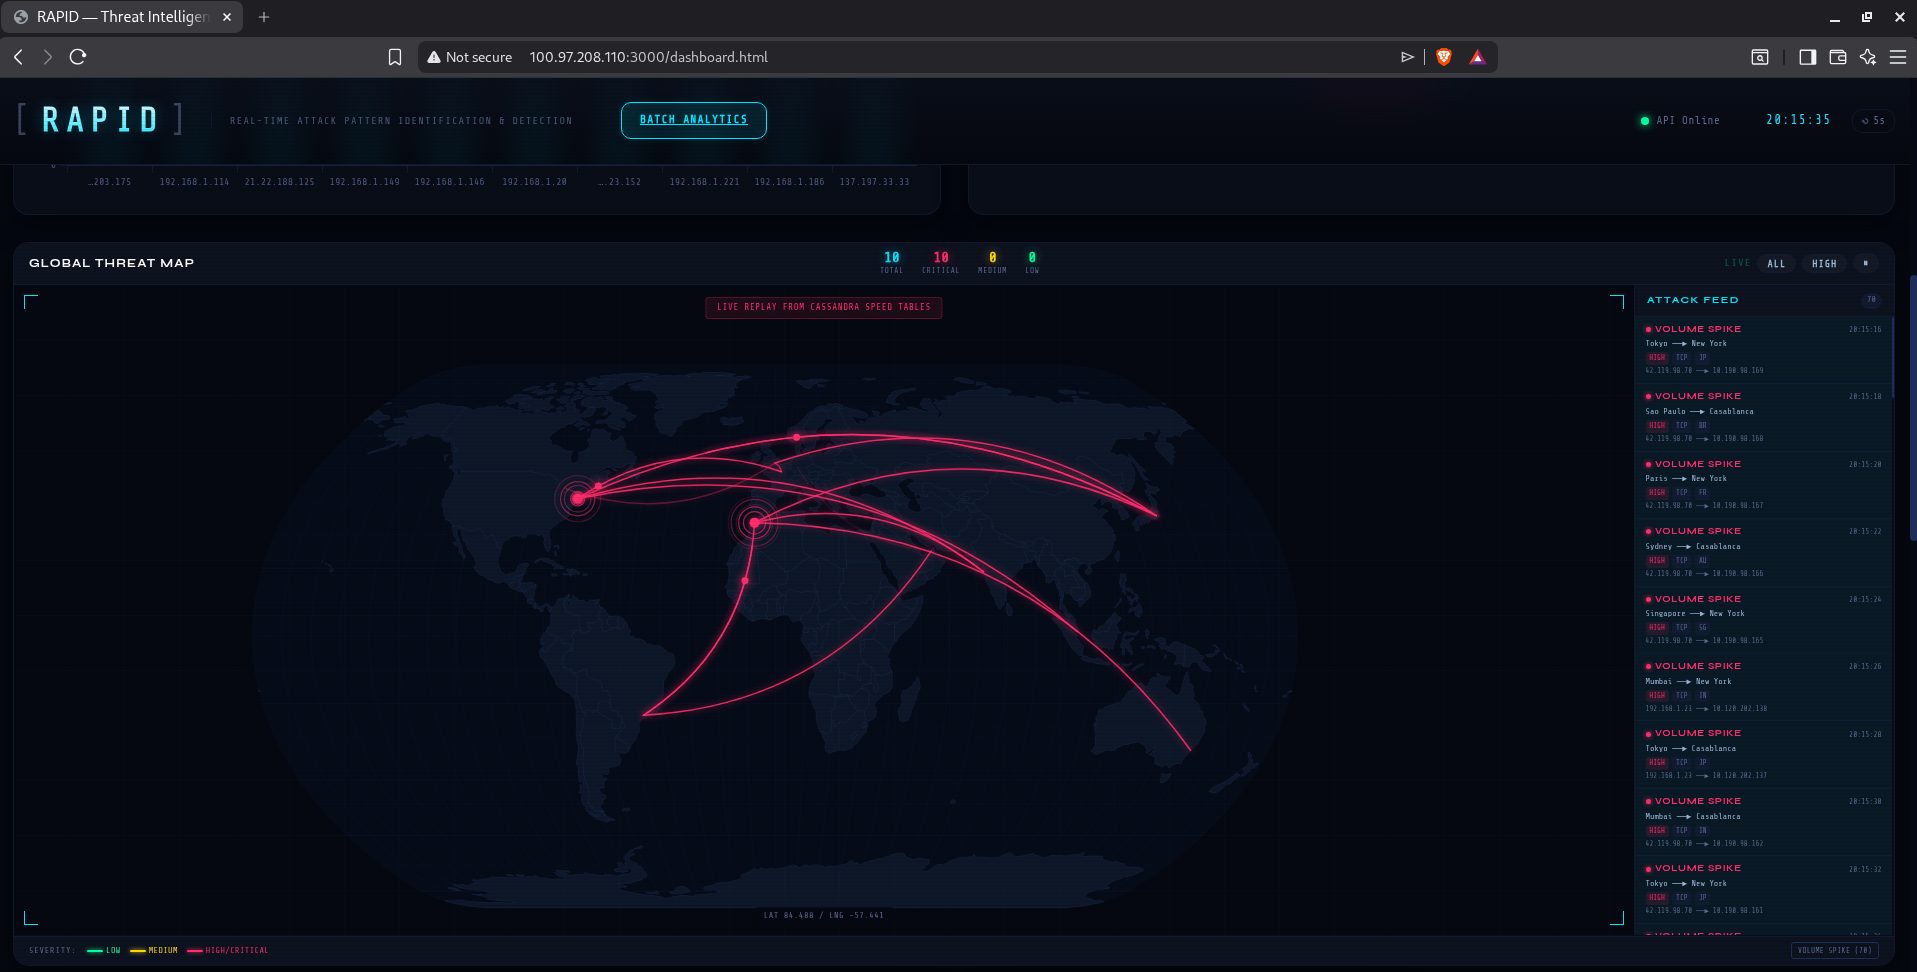
\includegraphics[width=\textwidth]{figures/serving/speed_dashboard/speed_dashboard_global_threat_map.png}
    \caption{Global threat map displaying attack trajectories and the real-time event flow.}
    \label{fig:speed-dashboard-global-map}
\end{figure}

The \textit{Attack Timeline} is a line chart built on the frontend from the scores, volume alerts, signature alerts and real-time threats already loaded. The \textit{Volume Alerts} and \textit{Signature Alerts} tables complement this reading by respectively detailing threshold exceedances and detections associated with signatures.

Figure~\ref{fig:speed-dashboard-timeline-alerts} validates the simultaneous display of the timeline, volume alerts and signature alerts.

\begin{figure}[H]
    \centering
    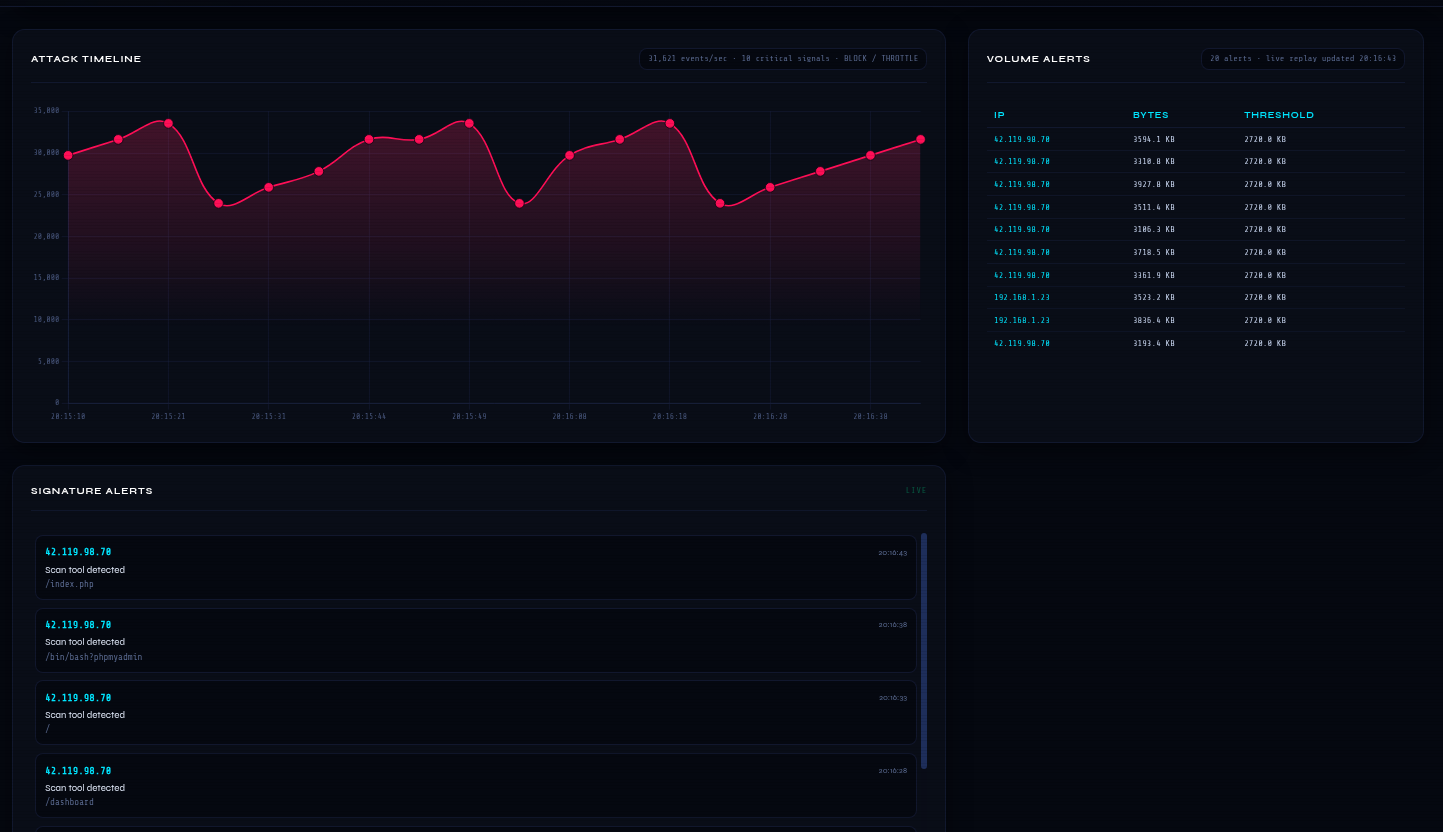
\includegraphics[width=\textwidth]{figures/serving/speed_dashboard/speed_dashboard_timeline_alerts.png}
    \caption{Attack timeline, volume alerts and signature alerts in the real-time view.}
    \label{fig:speed-dashboard-timeline-alerts}
\end{figure}

The \textit{Realtime Decision Queue} aggregates the sources returned by \texttt{/threats/top10?limit=50} and \texttt{/threats/realtime?limit=50}. It organizes IPs according to their score, number of evidences, severity and available consultation action.

This view synthesizes priority sources and facilitates decision-making through the score, number of evidences and severity level.

\begin{figure}[H]
    \centering
    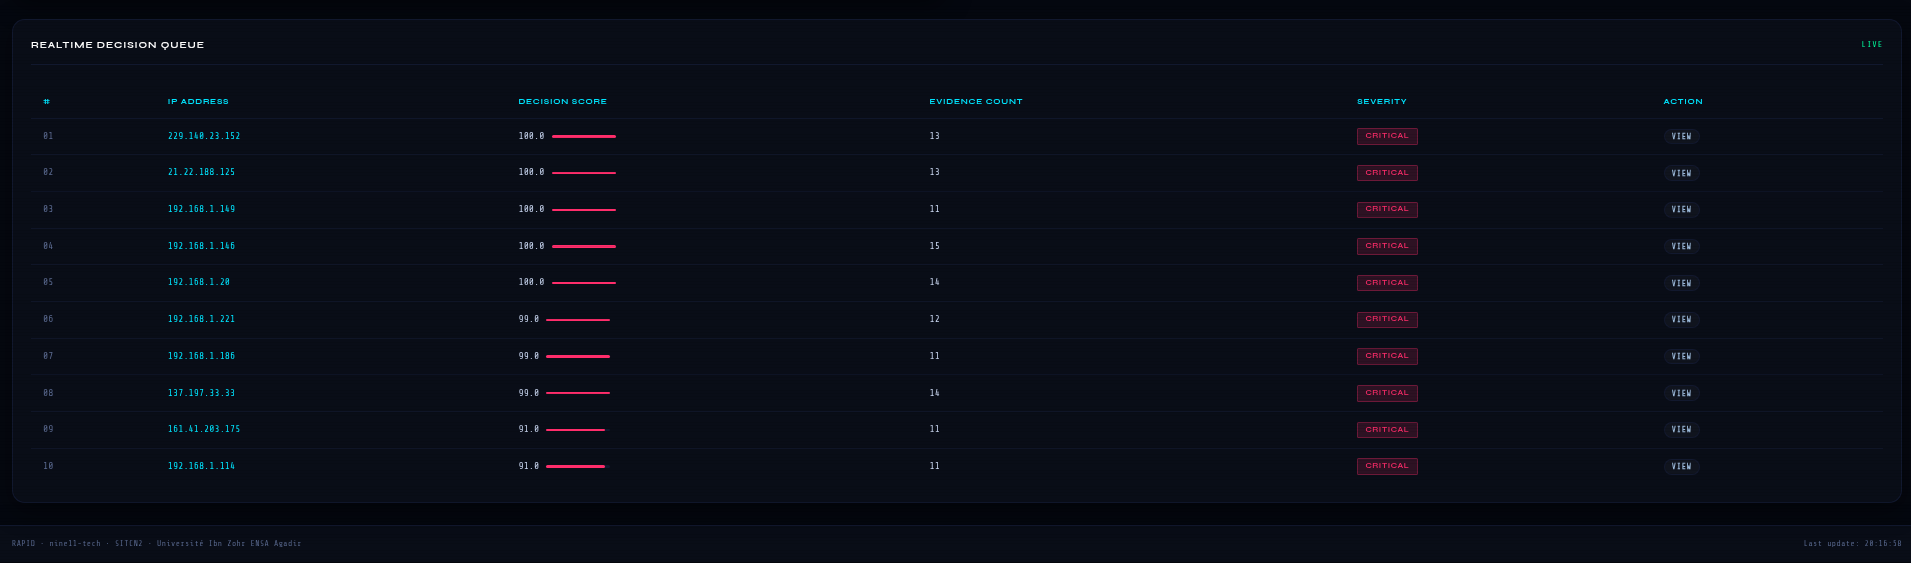
\includegraphics[width=\textwidth]{figures/serving/speed_dashboard/speed_dashboard_decision_queue.png}
    \caption{Real-time decision queue ranking IP addresses by score, evidences and severity.}
    \label{fig:speed-dashboard-decision-queue}
\end{figure}

In the batch view, the \textit{Batch Threat Timeline} chart is a stacked bar chart that represents historical events by day and by threat label. The \textit{Threat Volume} chart compares traffic volumes by category. The \textit{Attack Pattern Types} donut shows the distribution of detected attack families.

This screenshot shows how HBase views are transformed into summary charts: traffic volume by threat class and distribution of attack patterns.

\begin{figure}[H]
    \centering
    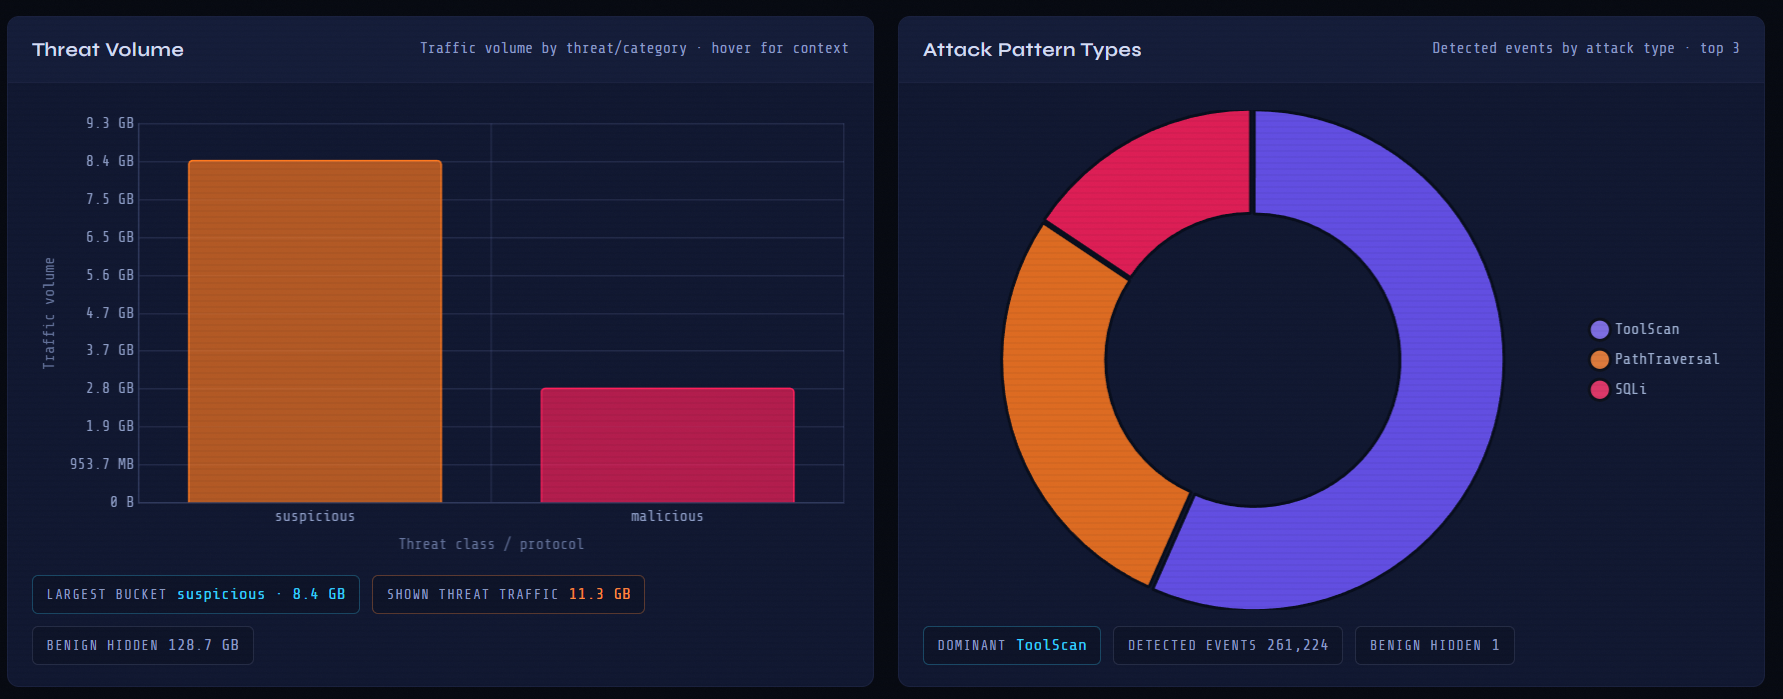
\includegraphics[width=\textwidth]{figures/serving/batch_dashboard/batch_dashboard_volume_patterns.png}
    \caption{Batch charts representing traffic volume by threat category and the distribution of attack families.}
    \label{fig:batch-dashboard-volume-patterns}
\end{figure}

The \textit{IP Reputation Scores -- HBase} chart horizontally ranks IPs according to a decision score recomputed on the frontend from reputation, exploitation indicators and event volume. The \textit{Top Port Scan Sources} chart aggregates scan records by IP and computes a score based on the number of distinct ports, connections and repetition of records.

Figure~\ref{fig:batch-dashboard-portscan-reputation} relates port scan sources to the IP reputation ranking in order to prioritize historical investigations.

\begin{figure}[H]
    \centering
    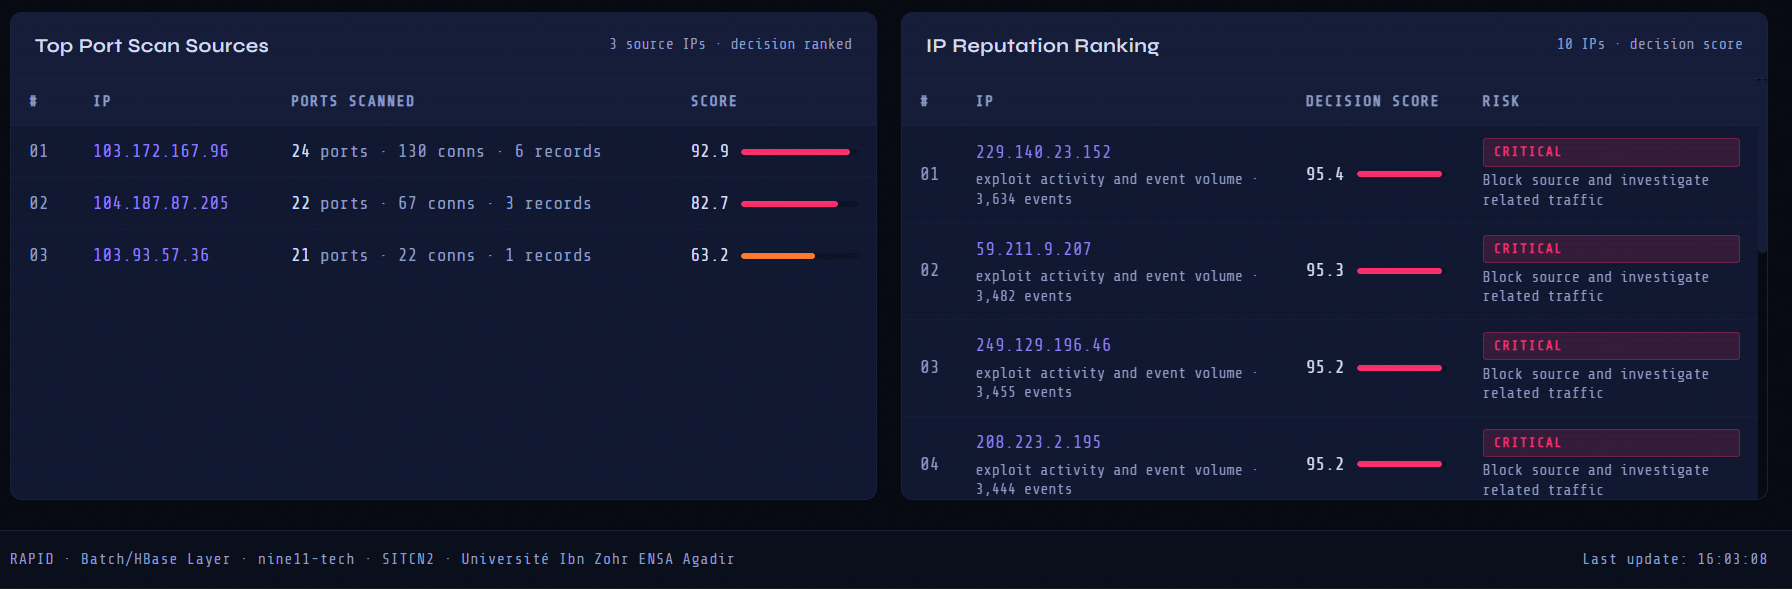
\includegraphics[width=\textwidth]{figures/serving/batch_dashboard/batch_dashboard_portscan_reputation_summary.png}
    \caption{Batch summary of the main port scan sources and the IP address reputation ranking.}
    \label{fig:batch-dashboard-portscan-reputation}
\end{figure}

\begingroup
\scriptsize
\setlength{\tabcolsep}{4pt}
\renewcommand{\arraystretch}{1.30}
\begin{longtable}{|
    >{\raggedright\arraybackslash\bfseries}p{0.23\textwidth}|
    >{\raggedright\arraybackslash}p{0.31\textwidth}|
    >{\raggedright\arraybackslash}p{0.34\textwidth}|
}
    \caption{Summary of dashboard visualizations.}
    \label{tab:dashboard-visualisations}\\
    \hline
    \tablehead{UI Element} & \tablehead{Consumed Data} & \tablehead{Role in the Analysis} \\
    \hline
    \endfirsthead
    \hline
    \tablehead{UI Element} & \tablehead{Consumed Data} & \tablehead{Role in the Analysis} \\
    \hline
    \endhead
    Speed KPI cards & \servingcell{\texttt{/threats/top10}, \texttt{/threats/volume-alerts},\\
    \texttt{/threats/recent}, \texttt{/threats/realtime},\\
    \texttt{/threats/threshold}} & Summarize the activity volume, maximum score, unique IPs, latest activity, adaptive threshold and number of volume alerts. \\
    \hline
    Top Realtime Risk Sources & \servingcell{\texttt{/threats/top10?limit=50}\\
    \texttt{/threats/realtime?limit=50}} & Identify the riskiest source IPs in the speed layer and prioritize decisions. \\
    \hline
    Attack Timeline & \servingcell{Signals already loaded from \texttt{top10}, \texttt{volume-alerts}, \texttt{recent} and \texttt{realtime}} & Represent a synthetic temporal pressure of events and critical signals. \\
    \hline
    Live Detection Mix & \servingcell{Signals already loaded from \texttt{top10}, \texttt{volume-alerts}, \texttt{recent} and \texttt{realtime}} & Show the composition of recent detections: scores, signatures, volume and brute force. \\
    \hline
    Global Threat Map & \servingcell{\texttt{/threats/geo/attacks};\\
    fallback on already loaded speed signals} & Visualize geographic trajectories, severity and attack types in a map flow. \\
    \hline
    Volume Alerts & \servingcell{\texttt{/threats/volume-alerts}\\
    \texttt{?limit=50}} & List IPs that exceed a volume threshold and compare the observed volume with the threshold. \\
    \hline
    Signature Alerts & \servingcell{\texttt{/threats/recent}\\
    \texttt{?limit=50}} & Display alerts derived from signatures, with reason, path or user agent. \\
    \hline
    Realtime Decision Queue & \servingcell{\texttt{/threats/top10?limit=50}\\
    \texttt{/threats/realtime?limit=50}} & Rank IPs by score, number of evidences, severity and consultation action. \\
    \hline
    Batch KPI cards & Main \texttt{/batch/*} endpoints & Count the available historical views: patterns, reputations, scans, multi-step chains, volumes and tables. \\
    \hline
    Batch Threat Timeline & \servingcell{\texttt{/batch/threat-timeline}\\
    \texttt{?limit=50}} & Observe the historical evolution of threats by day and by label. \\
    \hline
    Threat Volume & \servingcell{\texttt{/batch/threat-volume}\\
    \texttt{?limit=10}} & Compare traffic volumes by threat category and identify the largest buckets. \\
    \hline
    Attack Pattern Types & \servingcell{\texttt{/batch/attack-patterns}\\
    \texttt{?limit=30}} & Summarize the distribution of attack families: SQLi, XSS, Path Traversal, ToolScan or other patterns. \\
    \hline
    IP Reputation Ranking & \servingcell{\texttt{/batch/ip-reputation}\\
    \texttt{?limit=30}} & Rank historical IPs according to their reputation score and risk level. \\
    \hline
    Top Port Scan Sources & \servingcell{\texttt{/batch/port-scans/top?limit=10}\\
    \texttt{/batch/port-scans?limit=30}} & Identify the sources that scan the most ports and preserve the associated raw records. \\
    \hline
    Multi-Step Attack Chains & \servingcell{\texttt{/batch/multistep-attacks}\\
    \texttt{?limit=30}} & Highlight IPs that combine several attack stages in the history. \\
    \hline
    Modales de détail IP & \servingcell{\texttt{/threats/ip/}\\\texttt{\textless{}ip\textgreater{}}\\
    batch endpoints by IP} & Group the evidence associated with a source and facilitate the analyst's decision. \\
    \hline
\end{longtable}
\endgroup

This table details the attack patterns extracted from the batch views and makes it possible to identify dominant families, their severity and their decision score.

\begin{figure}[H]
    \centering
    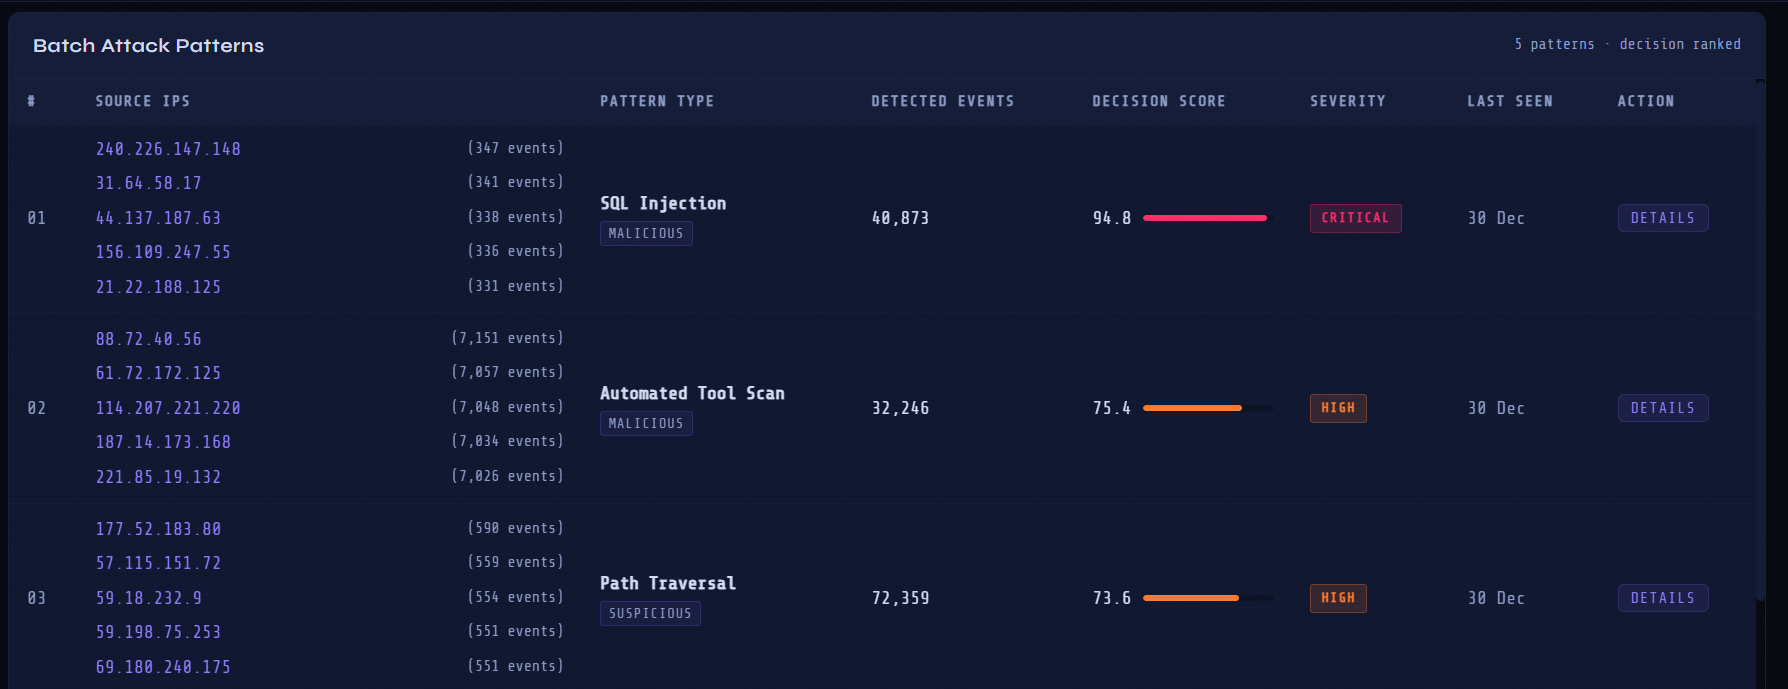
\includegraphics[width=\textwidth]{figures/serving/batch_dashboard/batch_dashboard_attack_patterns_table.png}
    \caption{Batch table detailing attack families, decision scores, severities and latest observations.}
    \label{fig:batch-dashboard-attack-patterns-table}
\end{figure}

The IP reputation table presents the historical scores computed from HBase views and provides direct decision support for the riskiest sources.

\begin{figure}[H]
    \centering
    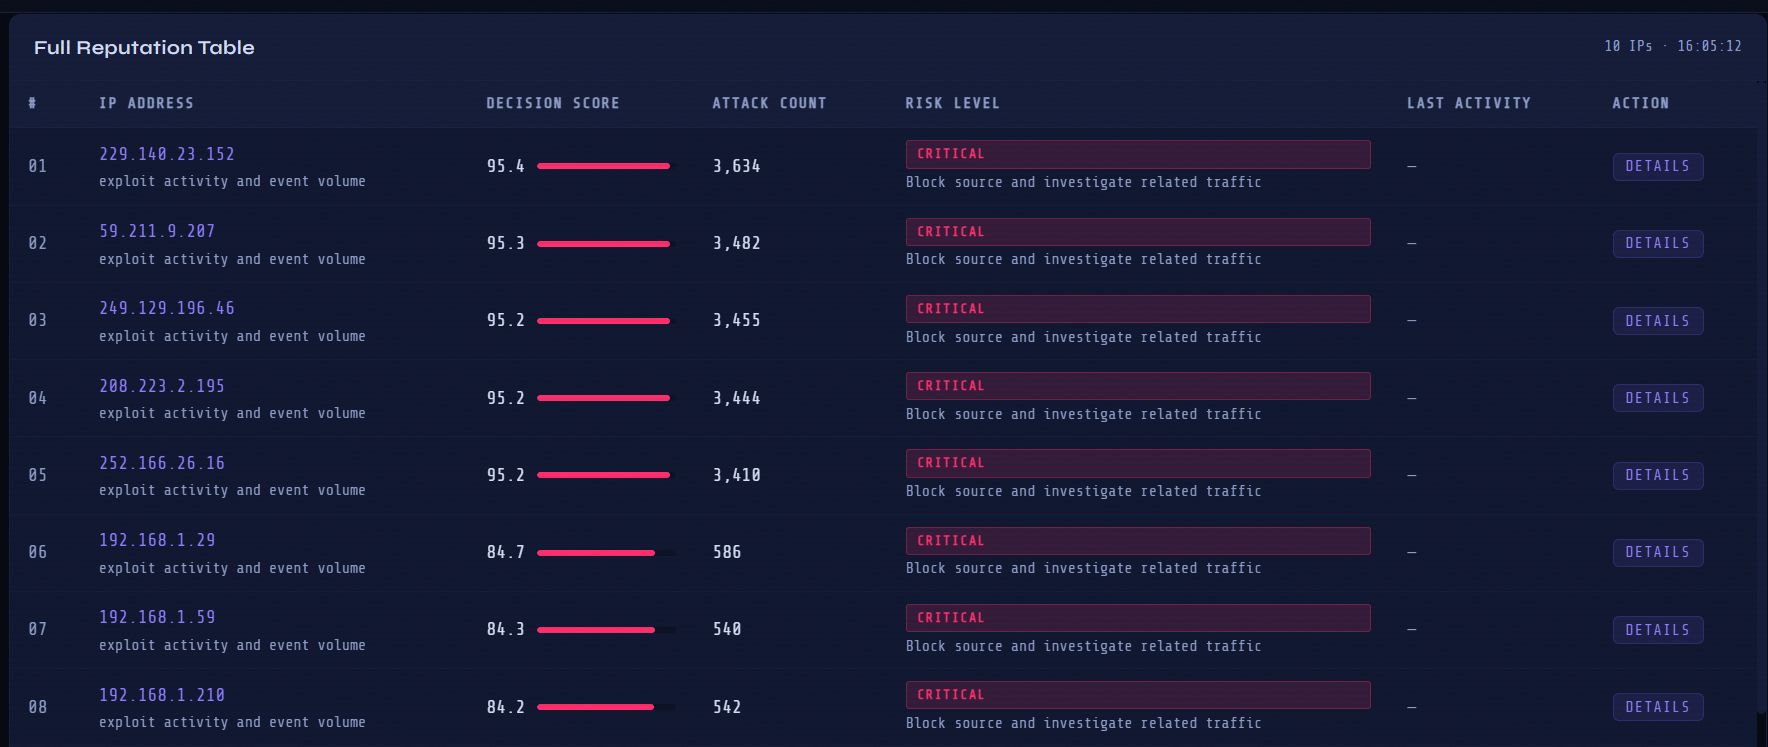
\includegraphics[width=\textwidth]{figures/serving/batch_dashboard/batch_dashboard_ip_reputation_table.png}
    \caption{Complete IP reputation table showing historical scores, risk levels and action recommendations.}
    \label{fig:batch-dashboard-ip-reputation-table}
\end{figure}

This screenshot illustrates detailed port scan records, making it possible to move from an aggregated view to the raw historical observations served by HBase.

\begin{figure}[H]
    \centering
    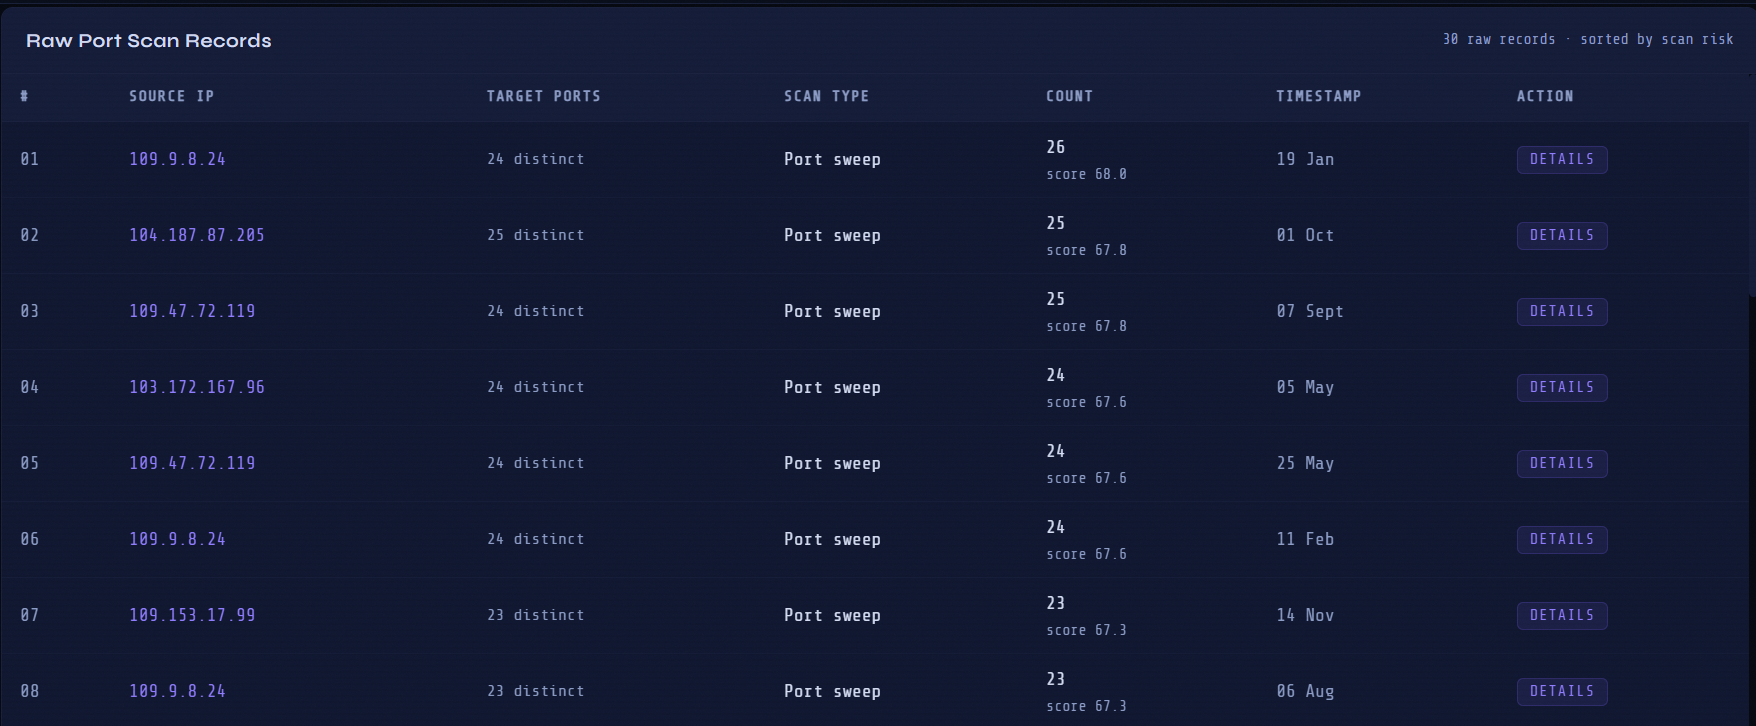
\includegraphics[width=\textwidth]{figures/serving/batch_dashboard/batch_dashboard_raw_port_scan_records.png}
    \caption{Batch port scan records with targeted ports, scan type, counter and observed period.}
    \label{fig:batch-dashboard-raw-port-scans}
\end{figure}

Figure~\ref{fig:batch-dashboard-multistep-chains} shows multi-step correlations, for example ToolScan, then SQLi and Path Traversal, in order to identify structured behaviors on the same IP.

\begin{figure}[H]
    \centering
    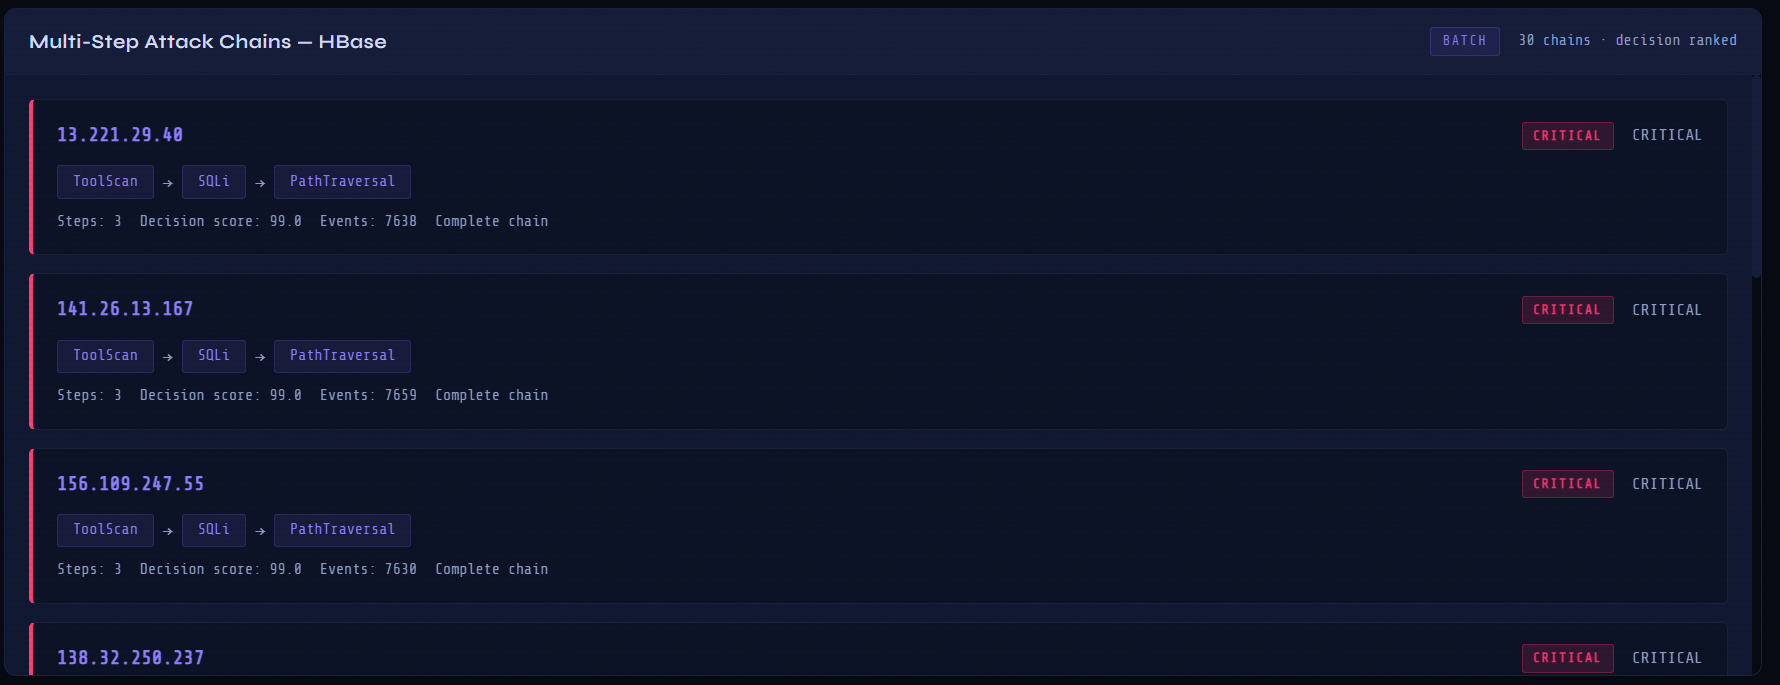
\includegraphics[width=\textwidth]{figures/serving/batch_dashboard/batch_dashboard_multistep_attack_chains.png}
    \caption{Multi-step attack chains detected in HBase with attack sequence, decision score and criticality level.}
    \label{fig:batch-dashboard-multistep-chains}
\end{figure}

\section{Separation between Batch and Speed Views}

The separation between batch and speed remains visible in the frontend, but it does not burden the user with internal computation details. Historical views come from HBase and are displayed in \texttt{batch.html}. They correspond to long-term memory produced by Spark batch processing: IP reputation, attack patterns, timeline, volume, scans and multi-step chains. Real-time results come from Cassandra and are displayed in \texttt{dashboard.html}. They represent the recent operational state: scores, signature alerts, volume alerts, active threats and adaptive threshold.

The dashboard merges these two perspectives at the user experience level. An IP can be studied from the speed view with \texttt{/threats/ip/<ip>}, which exposes both the recent state and a historical score. It can also be studied from the batch view with the HBase endpoints specific to the IP. In both cases, the frontend consumes already structured API responses. It does not need to know the Spark steps, the exact Cassandra tables, or the HBase scans performed by the backend. This separation respects the principle of the Lambda Architecture: the batch layer provides historical depth, the speed layer provides freshness, and the serving layer presents both in an exploitable form.

\section{Visual Validation of the Dashboard}

The screenshots integrated into this chapter validate the two temporalities of the serving layer. The speed views show the real-time indicators from Cassandra, the global map, the timeline, the alerts and the decision queue. The batch views show the historical results served from HBase: batch timeline, volumes, attack patterns, IP reputation, port scans and multi-step chains. This visual validation confirms that the results computed by the batch and speed layers are effectively accessible in the final interface.

\section{Chawi's Contribution to the Serving Layer}

Chawi's contribution in this layer concerns the final availability of analytical results. It includes the static dashboard, the visual presentation of results, the connection between API responses and HTML/JS components, and the hosting of the interface in the \texttt{chawi} profile with the \texttt{nginx-dashboard} container. This responsibility complements his role on HBase and Cassandra: the data are not only stored in NoSQL databases, they become queryable through an interface ready for demonstration.

More precisely, Chawi ensures the presentation part of the serving layer. The \texttt{batch.html}, \texttt{dashboard.html}, \texttt{batch.js}, \texttt{main.js}, \texttt{batch.css} and \texttt{style.css} files define the structure, charts, statistic cards, tables and modals. JavaScript transforms JSON responses into visible components: KPI values, score bars, severity badges, alert feeds, sorted tables and Chart.js charts. This contribution connects the results of the Lambda Architecture to an operational reading understandable by an analyst.

\section{Summary}

The RAPID serving layer transforms the technical outputs of the pipeline into an analysis interface. HBase provides the historical batch views, Cassandra provides the recent speed results, Flask exposes the REST endpoints, and the HTML/JavaScript dashboard displays information as cards, charts, tables, alerts and interactive maps. This organization keeps the frontend simple: it consumes API responses and updates the DOM, without carrying the details of Spark processing or NoSQL queries.

The dashboard therefore fulfills an essential function in the project. It verifies that the results are not only computed, but also served and interpretable. The separation between \texttt{batch.html} and \texttt{dashboard.html} makes the historical/real-time duality explicit, while IP searches and detail modals bring these two temporalities together at decision time.

\section{Bonus Features}
\label{sec:bonus}

The assignment proposes several bonus improvements: machine learning, event correlation, geolocation, and adaptive scoring. RAPID implements or demonstrates all of them in a way that extends the main Lambda Architecture.

\subsection{Machine Learning Classification}

The \texttt{ml\_bonus.py} script trains a Spark MLlib Random Forest classifier to predict \texttt{threat\_label} from features such as transferred bytes, protocol, action, and log type. The objective is not to replace rule-based detection, but to show that the same Big Data pipeline can support statistical classification. The model reached about 92\% global accuracy, while the report also recognizes that class imbalance can hide errors on minority malicious classes.

\begin{figure}[H]
    \centering
    
\includegraphics[width=0.92\textwidth]{\detokenize{figures/bonus_features/Screenshot 2026-05-07 172733.png}}
    \caption{Spark MLlib model evaluation and saved prediction output.}
    \label{fig:ml-results}
\end{figure}

\subsection{Multi-Step Attack Correlation}

The batch layer includes a multi-step detector that correlates different attack families for the same source IP. For example, a source that performs tool scanning, SQL injection, and path traversal is more dangerous than a source with one isolated event. This bonus improves the quality of historical prioritization.

\begin{figure}[H]
    \centering
    
\includegraphics[width=0.90\textwidth]{\detokenize{figures/bonus_features/3.png}}
    \caption{Enriched multi-step attack correlation with risk level.}
    \label{fig:multistep}
\end{figure}

\subsection{Adaptive Threshold and Geolocation-Oriented View}

The API includes an adaptive threshold calculation based on recent activity. Instead of relying only on a fixed score, the system compares an IP against the current context of the platform. The dashboard also includes a global map view for attack visualization, which supports the geolocation improvement proposed in the assignment.

\begin{figure}[H]
    \centering
    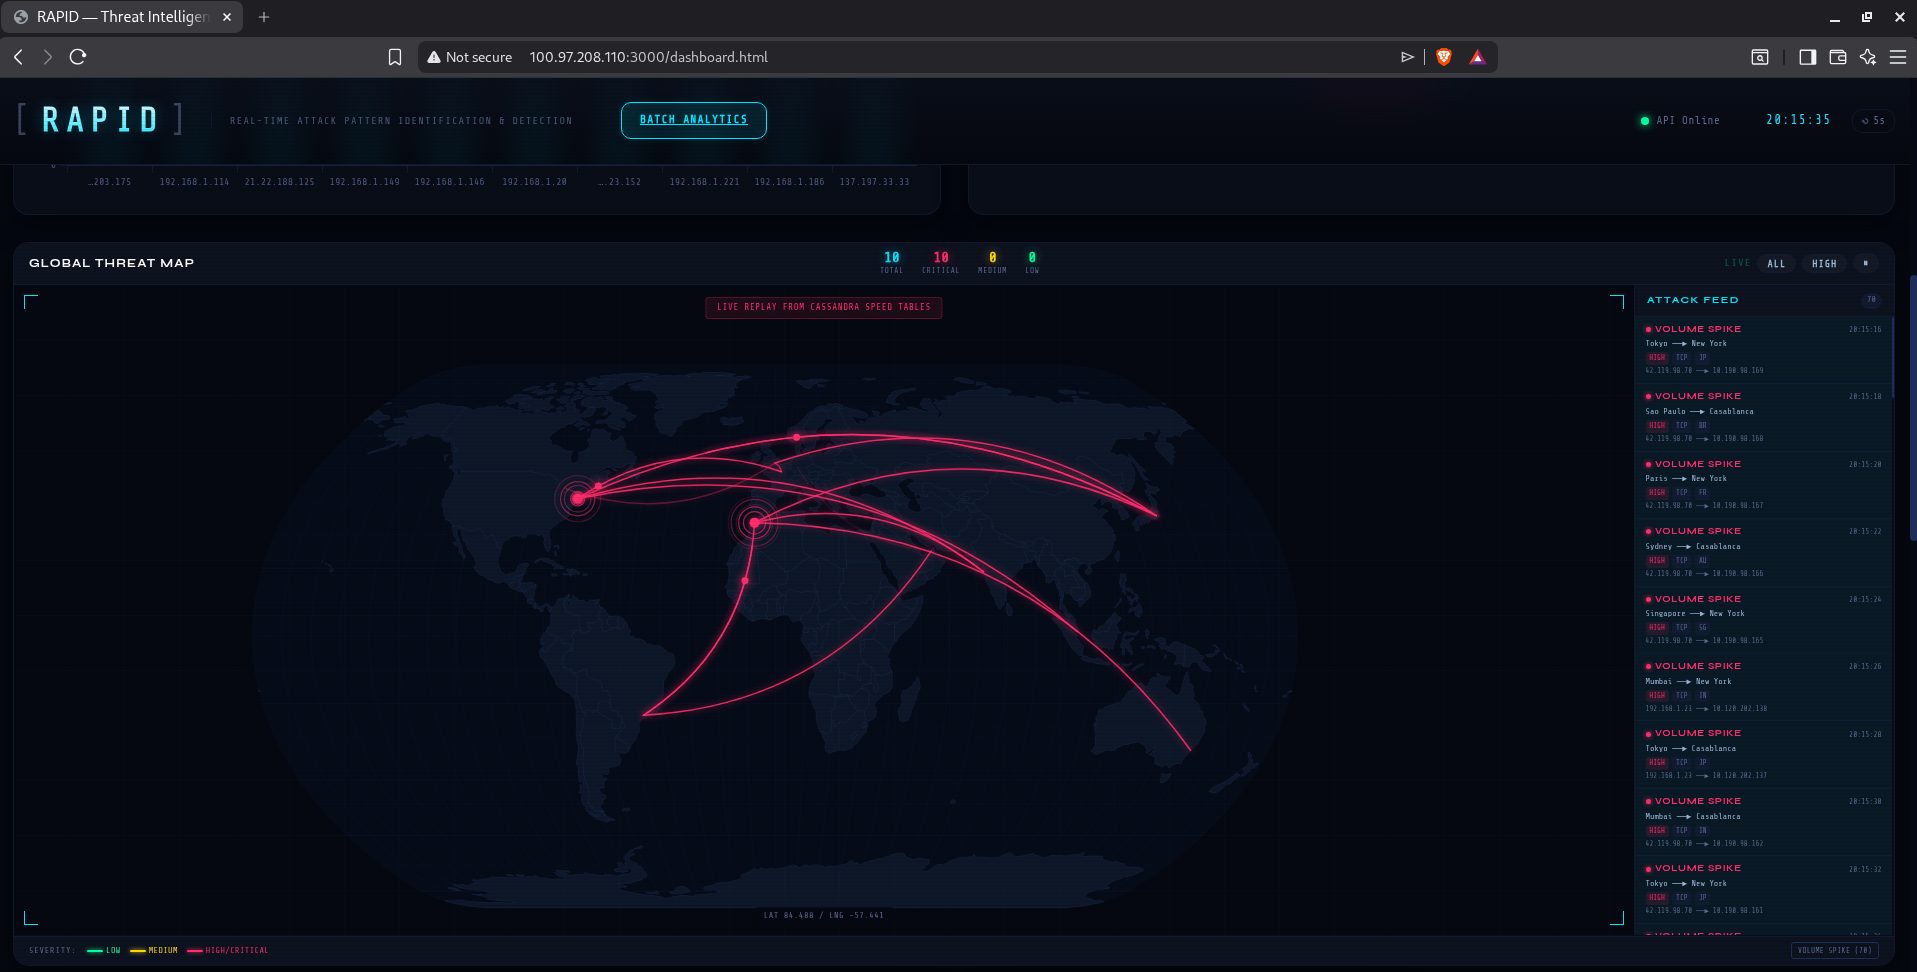
\includegraphics[width=0.92\textwidth]{figures/serving/speed_dashboard/speed_dashboard_global_threat_map.png}
    \caption{Global threat map used to visualize attack origins and trajectories.}
    \label{fig:global-map}
\end{figure}

These bonuses show that RAPID is extensible. New detectors can be added as Spark jobs, new serving views can be materialized in HBase or Cassandra, and the API can expose new indicators without changing the core architecture.

\section{Conclusion}
\label{sec:conclusion}

\subsection{Summary of Achievements}

This project successfully delivered a full-stack, production-inspired cybersecurity 
threat detection platform built on the Lambda Architecture. The following technical 
milestones were accomplished:

\begin{itemize}
    \item A \textbf{complete Lambda Architecture} was deployed, integrating HDFS, 
    Apache Kafka, Apache Spark (batch and streaming), HBase, Cassandra, and a 
    Flask REST API into a coherent data pipeline.
    
    \item \textbf{Five distinct threat categories} were implemented with detection 
    logic covering brute-force attacks, SQL injection, XSS signatures, port scanning, 
    and abnormal data exfiltration.
    
    \item \textbf{Real-time alerting latency} was measured at under five seconds 
    end-to-end, from log ingestion via Kafka to alert storage in Cassandra.
    
    \item The \textbf{batch layer} produced persistent reputation scores and 
    attack pattern summaries stored in HBase, enabling historical forensics at scale.
    
    \item A \textbf{Random Forest classifier} (bonus) achieved 92\% accuracy on 
    the \texttt{threat\_label} classification task, demonstrating the feasibility 
    of ML-augmented threat detection within the same pipeline.
    
    \item A \textbf{unified REST API} allowed consumers to query both the historical 
    batch view and the live speed layer for any given source IP, fulfilling the 
    serving layer requirement of the Lambda Architecture.
\end{itemize}

\subsection{Lessons Learned}

Several important technical insights emerged during development:

\begin{itemize}
    \item \textbf{Class imbalance is a critical concern in security datasets.} 
    The DuckDB analysis revealed a significant skew toward \textit{benign} traffic 
    in the dataset. Without addressing this imbalance (e.g., via SMOTE or 
    class-weighted training), ML models tend to over-predict the majority class, 
    yielding misleadingly high accuracy while missing actual threats.
    
    \item \textbf{Windowing semantics matter at scale.} Choosing between tumbling 
    and sliding windows in Spark Streaming has a direct impact on both detection 
    sensitivity and resource consumption. Brute-force detection required a sliding 
    window to avoid splitting attack bursts across window boundaries.
    
    \item \textbf{Schema design for the speed layer requires careful TTL planning.} 
    Cassandra's time-to-live (TTL) mechanism is essential for managing the 24-hour 
    active threat window; without it, the table grows unbounded under sustained 
    attack simulation.
    
    \item \textbf{The Lambda Architecture introduces operational complexity.} 
    Maintaining two separate code paths (batch and streaming) for similar logic 
    increases maintenance overhead. This motivates the alternative \emph{Kappa 
    Architecture}, which processes all data through a single streaming path.
\end{itemize}

\subsection{Future Improvements}

Several enhancements could significantly extend the platform's capabilities:

\begin{enumerate}
    \item \textbf{SMOTE for class rebalancing} — Applying Synthetic Minority 
    Oversampling Technique to the training set would improve the Random Forest 
    model's recall on \textit{malicious} and \textit{suspicious} classes, reducing 
    false negatives in production.
    
    \item \textbf{Multi-stage attack correlation} — Implementing a stateful event 
    correlation engine (e.g., using Apache Flink) could detect composite attack 
    chains such as reconnaissance $\rightarrow$ exploitation $\rightarrow$ lateral 
    movement, which are invisible to single-event rules.
    
    \item \textbf{GeoIP threat mapping} — Integrating a MaxMind GeoLite2 lookup 
    into the streaming pipeline would enable geographic visualization of attack 
    origins on the dashboard, adding operational value for SOC analysts.
    
    \item \textbf{Adaptive thresholds} — Rather than fixed rule thresholds 
    (e.g., ``5 failed logins''), a feedback loop based on rolling baseline 
    statistics per IP subnet would reduce both false positives in noisy environments 
    and false negatives during low-and-slow attacks.
    
    \item \textbf{Migration toward Kappa Architecture} — Replacing the separate 
    batch layer with a replayable Kafka-based stream would simplify the codebase 
    while retaining historical reprocessing capability, reducing the operational 
    burden of maintaining dual pipelines.
\end{enumerate}

\subsection{Closing Remarks}

This project demonstrated that modern Big Data tooling, when composed thoughtfully 
according to the Lambda Architecture, can form the foundation of a credible and 
extensible cybersecurity detection platform. The combination of deep batch analytics 
and sub-second streaming detection addresses a genuine operational need, and the 
modular design of the pipeline ensures that individual components can be upgraded 
or replaced independently as the threat landscape evolves.

\clearpage
\bibliographystyle{plain}
\bibliography{references}

\end{document}
